\begin{apendicesenv}

%\partapendices

\chapter{Questionário de Pesquisa}
\label{ap:questionario}

\begin{figure}[htbp]
	\centering
	\subfigure[Questionário Parte 1]{
        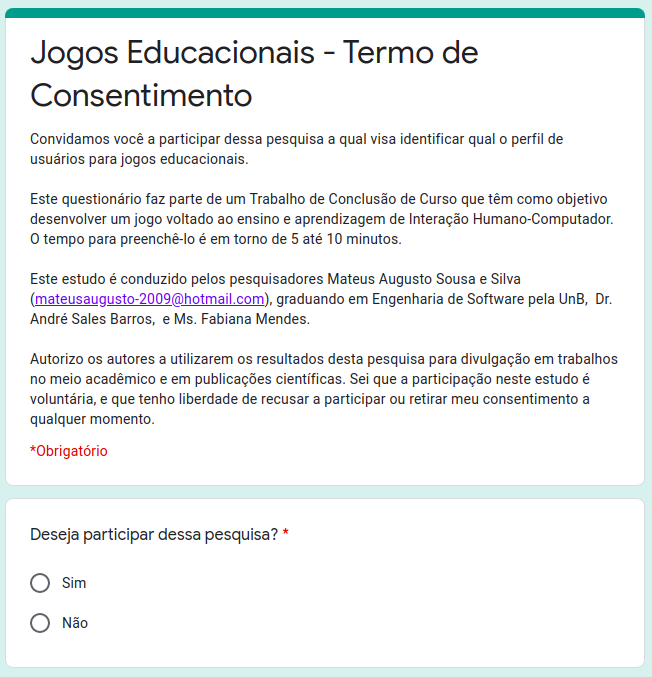
\includegraphics[keepaspectratio=true,scale=1.25]{figuras/apendice/survey1.png}
        \label{Fig:survey_pt1.png}
    }
    \quad
    \subfigure[Questionário Parte 2]{
        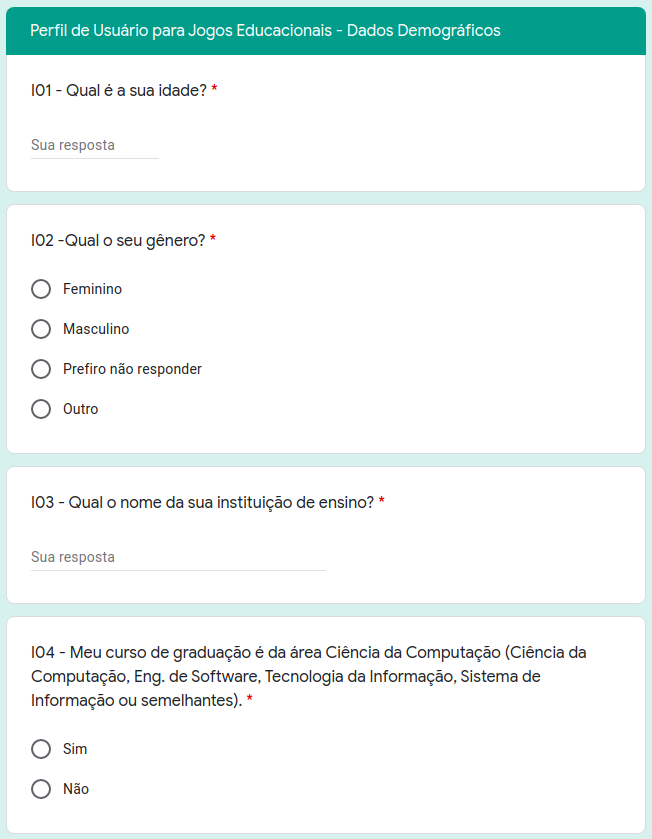
\includegraphics[keepaspectratio=true,scale=1.25]{figuras/apendice/survey2.png}
        \label{Fig:survey_pt2.png}
    }
    \quad
     \subfigure[Questionário Parte 3]{
        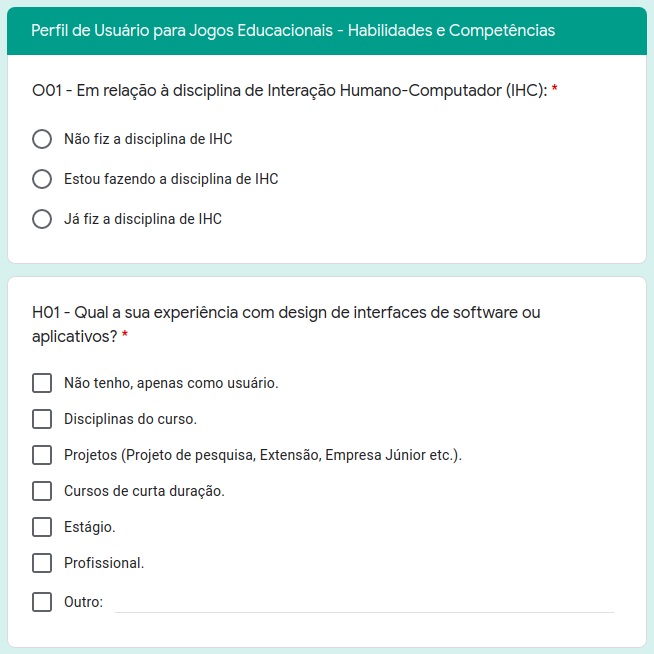
\includegraphics[keepaspectratio=true,scale=1.25]{figuras/apendice/survey3.png}
        \label{Fig:survey_pt3.png}
    }
    \quad
     \subfigure[Questionário Parte 4]{
        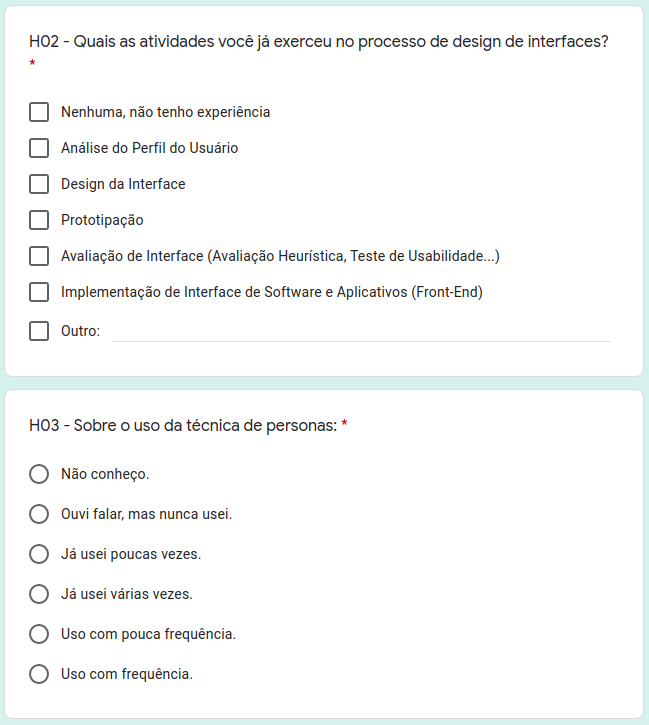
\includegraphics[keepaspectratio=true,scale=1.25]{figuras/apendice/survey4.png}
        \label{Fig:survey_pt4.png}
    }
   
	\caption{Questionário de Pesquisa 1-4 - Próprio Autor}
	\label{Fig:survey1.png}
\end{figure}

\begin{figure}[htbp]
	\centering
	\subfigure[Questionário Parte 5]{
        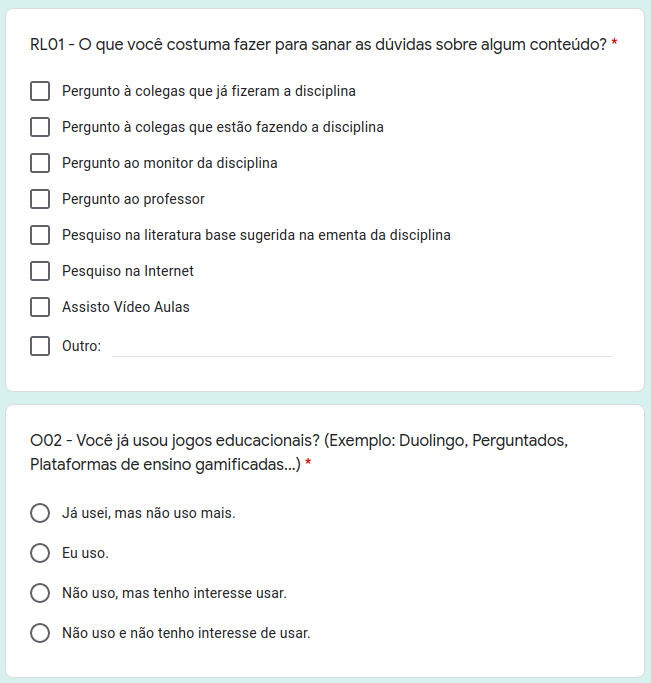
\includegraphics[keepaspectratio=true,scale=1.25]{figuras/apendice/survey5.png}
        \label{Fig:survey_pt5.png}
    }
    \quad
    \subfigure[Questionário Parte 6]{
        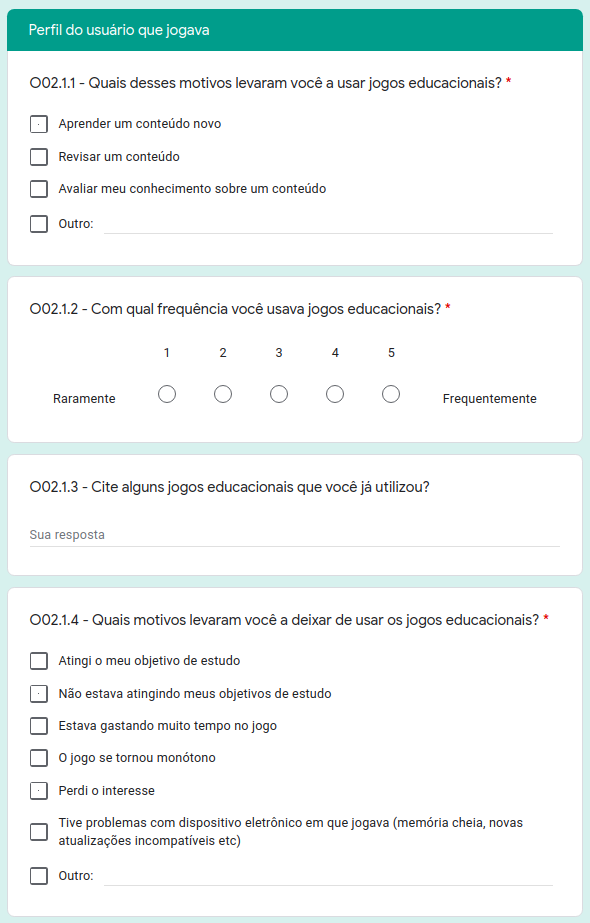
\includegraphics[keepaspectratio=true,scale=1.25]{figuras/apendice/survey6.png}
        \label{Fig:survey_pt6.png}
    }
    \quad
     \subfigure[Questionário Parte 7]{
        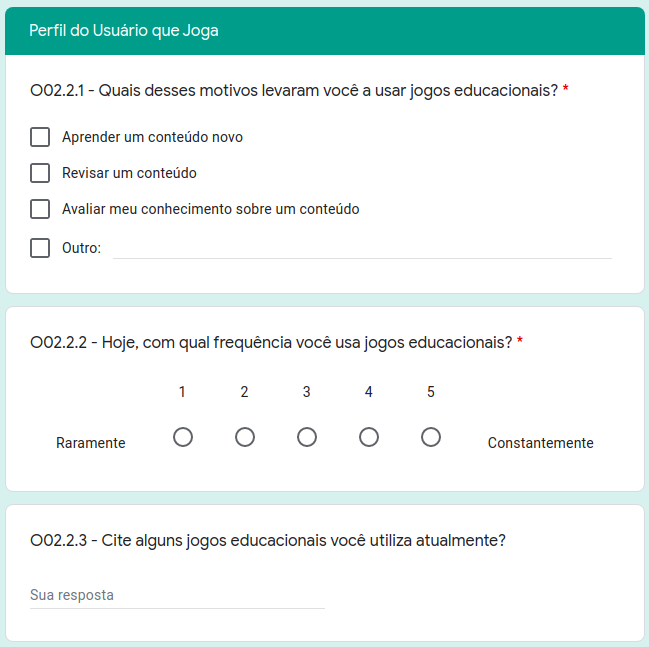
\includegraphics[keepaspectratio=true,scale=1.25]{figuras/apendice/survey7.png}
        \label{Fig:survey_pt7.png}
    }
    \quad
     \subfigure[Questionário Parte 8]{
        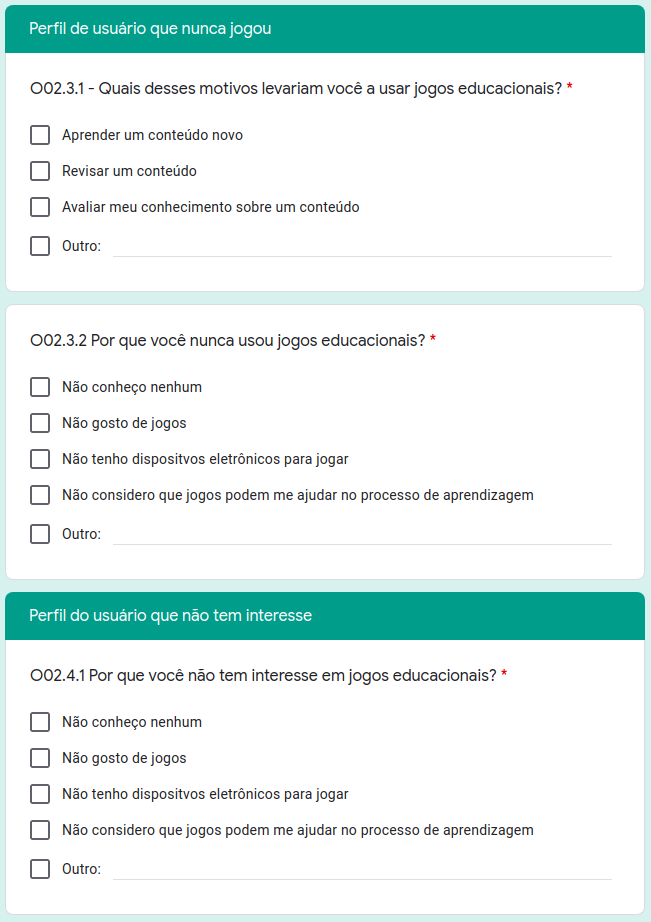
\includegraphics[keepaspectratio=true,scale=1.25]{figuras/apendice/survey8.png}
        \label{Fig:survey_pt8.png}
    }
   
	\caption{Questionário de Pesquisa 5-8 - Próprio Autor}
	\label{Fig:survey2.png}
\end{figure}

\begin{figure}[htbp]
	\centering
	\subfigure[Questionário Parte 9]{
        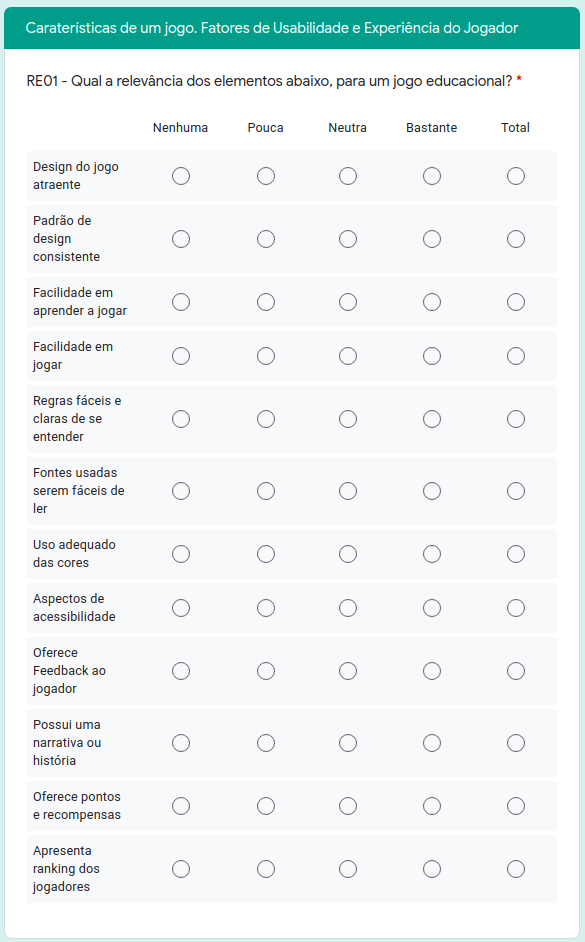
\includegraphics[keepaspectratio=true,scale=1.25]{figuras/apendice/survey9.png}
        \label{Fig:survey_pt9.png}
    }
    \quad
    \subfigure[Questionário Parte 10]{
        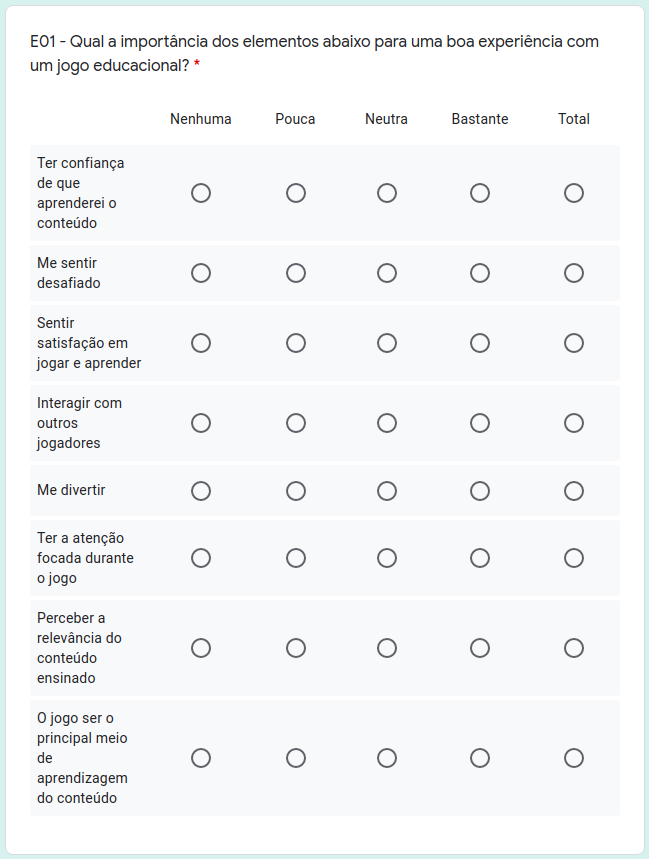
\includegraphics[keepaspectratio=true,scale=1.25]{figuras/apendice/survey10.png}
        \label{Fig:survey_pt10.png}
    }
    \quad
     \subfigure[Questionário Parte 11]{
        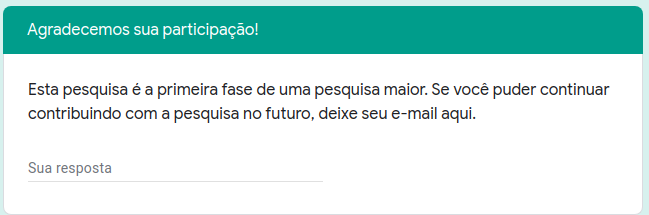
\includegraphics[keepaspectratio=true,scale=1.25]{figuras/apendice/survey11.png}
        \label{Fig:survey_pt11.png}
    }
   
	\caption{Questionário de Pesquisa 9-11 - Próprio Autor}
	\label{Fig:survey3.png}
\end{figure}

\chapter{Relatório de Execução e Resultados do Questionário de Pesquisa}
\label{ap:res_quest}

O objetivo deste \textit{Survey} foi de estabelecer uma base de dados para a construção das personas e levantar requisitos para o jogo. Como o foco deste estudo é voltado para o desenvolvimento de um jogo que auxilie o ensino da técnica de Personas, o público-alvo, o qual foi direcionado o questionário, foram alunos de graduação e pós-graduação de cursos da área de Ciência da Computação. Foi planejado para este estudo, um período de quatro semanas para a coleta dos dados, ou seja, a amostra de pesquisa foram os respondentes do dia 06/10/2020 ao dia 27/10/2020. 

As perguntas do questionário foram elaboradas baseando-se na literatura revista. Foram utilizados o modelo de personas descrito no artigo em "\citeauthor{usability2020}", os atributos das personas descritas por \citeonline{barbosa_silva}, as características de jogos sérios em IHC identificados por \citeonline{deSales_SousaeSilva_2020} e as metas de experiência do jogador descritas por \citeonline{Petri_Wangenheim_2019}. Além da origem, a seguir são apresentados na Tabela \ref{tab:Table_survey} os objetivos de cada questão referenciada por um identificador.

%longtable

\begin{table}[ht]
\centering
\caption{Rastreabilidade do Questionário}
\label{tab:Table_survey}
\begin{tabular}{|l|l|l|}
\hline
\textbf{ID} & \textbf{Objetivos}                                              & \textbf{Origem}   \\ \hline
I01         & - Usar como base para caracterização das personas               & UG, HC            \\ \hline
I02         & - Usar como base para caracterização das personas               & UG, HC            \\ \hline
I03         & - Usar como base para caracterização das personas               & UG, HC            \\ \hline
I04         & \begin{tabular}[c]{@{}l@{}}
              - Usar como base para caracterização das personas.\\ 
              - Controlar se respondente se enquadra no perfil do público-alvo
              \end{tabular}                                                   & UG, HC            \\ \hline
O01         & \begin{tabular}[c]{@{}l@{}}
              - Auxiliar na identificação dos objetivos das personas \\ 
              - Identificar o nível de conhecimento das personas
              \end{tabular}                                                   & UG, HC            \\ \hline
H01         & \begin{tabular}[c]{@{}l@{}}- Identificar o nível de conhecimento das personas \\ 
              - identificar as habilidades das personas
              \end{tabular}                                                   & UG, HC            \\ \hline
H02         & \begin{tabular}[c]{@{}l@{}}
              - Identificar o nível de conhecimento das personas \\ 
              - identificar as habilidades das personas
              \end{tabular}                                                 & UG, HC              \\ \hline
H03         & \begin{tabular}[c]{@{}l@{}} 
              - Auxiliar na validação da oportunidade de intervenção proposta\\ neste trabalho.
              \end{tabular} & UG, HC                                                              \\ \hline
RL01        & - Identificar com quem a persona se relaciona                   & HC                \\ \hline
O02         & \begin{tabular}[c]{@{}l@{}} 
              - Auxiliar na identificação dos objetivos das personas   \\       
              - Auxiliar na validação da oportunidade de intervenção proposta\\ neste trabalho.
              \end{tabular} & UG, HC            \\ \hline
O02.1.1     & - Identificar objetivos das personas                            & UG, HC            \\ \hline
O02.1.2     & \begin{tabular}[c]{@{}l@{}}
              - Auxiliar na identificação dos objetivos das personas\\ 
              - Identificar característica da tarefa realizada pela persona
              \end{tabular}                                                   & UG, HC            \\ \hline
O02.1.3     & - Usar como base para levantamento de alguns requisitos         &   -               \\ \hline
O02.1.4     & - Auxiliar na identificação dos objetivos das personas          & UG, HC            \\ \hline
O02.2.1     & - Identificar objetivos das personas                            & UG, HC            \\ \hline
O02.2.2     & \begin{tabular}[c]{@{}l@{}}
              - Auxiliar na identificação dos objetivos das personas\\ 
              - Identificar característica da tarefa realizada pela persona
              \end{tabular}                                                   & UG, HC            \\ \hline
O02.2.3     & - Usar como base para levantamento de alguns requisitos         &   -               \\ \hline
O02.3.1     & - Identificar objetivos das personas                            & UG, HC            \\ \hline
O02.3.2     & - Auxiliar na identificação dos objetivos das personas                    & UG, HC  \\ \hline
O02.4.1     & - Auxiliar na identificação dos objetivos das personas                    & UG, HC  \\ \hline
RE01        & - Identificar requisitos para o jogo                                      & \begin{tabular}[c]{@{}l@{}}
                                                                                          UG, HC, \\ 
                                                                                          JS, ME
                                                                                         \end{tabular}  \\ \hline
E01         & \begin{tabular}[c]{@{}l@{}}
              - Identificar requisitos para o jogo\\ 
              - Definir as metas de experiência do jogador\end{tabular}                & \begin{tabular}[c]{@{}l@{}}
                                                                                          UG, HC, \\ 
                                                                                          JS, ME
                                                                                         \end{tabular}  \\ \hline
\multicolumn{3}{p{15cm}}{\textbf{Legenda:} UG - \citeonline{usability2020}; HC - \citeonline{barbosa_silva} ; JS - \citeonline{deSales_SousaeSilva_2020}; ME - \citeonline{Petri_Wangenheim_2019}} \\
\end{tabular}
\end{table}

Antes da distribuição do questionário foi realizado um teste piloto com três pessoas. O objetivo do teste foi coletar \textit{feedbacks} sobre a compreensão e o layout das perguntas, a estrutura e o fluxo do questionário e também identificar erros e o tempo médio para se concluir o questionário. O teste piloto foi realizado de forma virtual, via plataforma de vídeo-chamada. Primeiramente o respondente recebeu algumas informações introdutórias sobre a pesquisa, em seguida ele acessou o questionário em seu computador e ativou o compartilhamento de tela. Dada a confirmação para o início da execução do questionário foram anotadas as percepções do avaliador enquanto o participante respondia. 

Concluído o teste piloto foi solicitado um relato oral do responte sobre sua percepção ao longo da execução do questionário, as quais foram anotadas pelo avaliador. Este processo foi realizado com cada um dos três participantes do teste piloto. Depois de analisadas as anotações, foram aplicadas as sugestões de melhoria e corrigidos os erros encontrados no questionário. 

Tendo o questionário já na sua versão final, este foi distribuído via alguns meios de comunicação virtuais, como mensagem de e-mail e redes sociais para a comunidade discente das instituições de ensino da Universidade de Brasília (UnB), Universidade Federal do Mato Grosso do Sul (UFMS), Universidade Federal do Amazonas (UFAM), Universidade Federal do Mato Grosso (UFMT) e Universidade Católica de Salvador (UCSAL). O questionário completo se encontra na seção de Apêndice \ref{ap:questionario}. 

Foram coletados os dados de 184 respondentes. Destes, foram identificados pelos endereços de e-mail fornecidos, que houveram oito pessoas que responderam ao questionário mais de uma vez, sendo assim estas foram descartadas. Restando 176 respondentes pode-se fazer uma análise preliminar dos dados obtidos. 

Dos respondentes, 134 são do sexo Masculino e 40 Feminino. Pode-se identificar que 1 respondente se declarou como de Outro sexo e 1 preferiu não responder. Segue a Figura \ref{Fig:genero.png}, dos sexos dos respondentes.

\begin{figure}[htbp]
	\centering
	\caption{Gênero dos respondentes}
	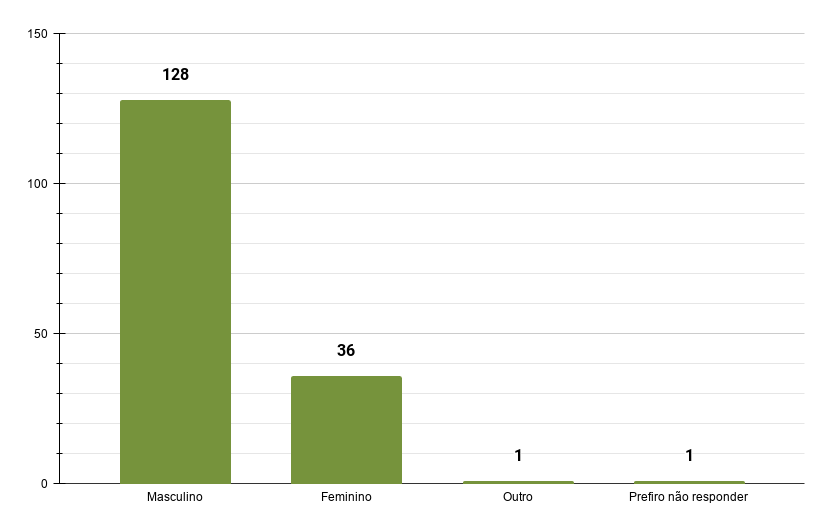
\includegraphics[keepaspectratio=true,scale=0.51]{figuras/apendice/graficos_survey/genero.png}
	\label{Fig:genero.png}
\end{figure}

Em relação à idade dos respondentes foi observado que a idade mínima foi de 18 anos e a máxima de 53 anos. A idade mais frequente foi a de 21 anos, com 30 respondentes. Não houveram respondentes com idades de 29, 33, 34, 37, 39, 41, 42, 43, 44, 45, 46, 48, 49, 50, 51 e 52 anos. A seguir, a Figura \ref{Fig:idade.png}, da idade dos respondentes.

\begin{figure}[htbp]
	\centering
	\caption{Relação da quantidade de respondentes por idade}
	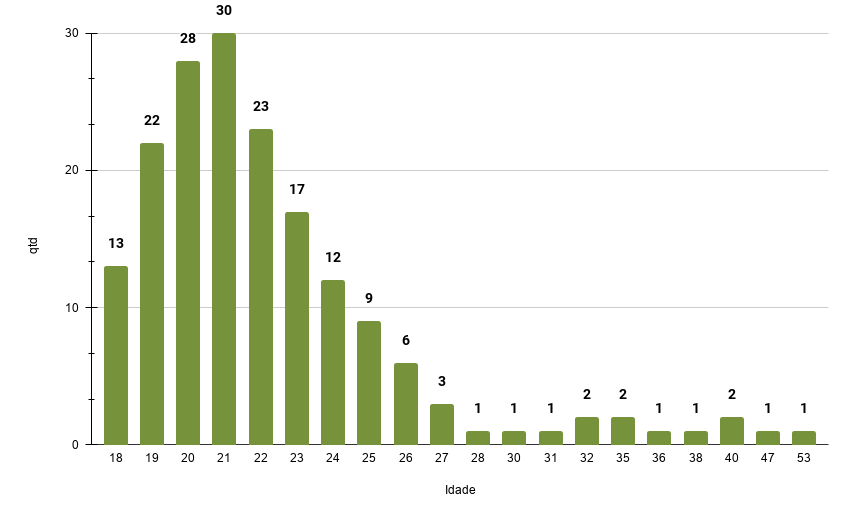
\includegraphics[keepaspectratio=true,scale=0.51]{figuras/apendice/graficos_survey/idade.png}
	\label{Fig:idade.png}
\end{figure}

Das Instituições de ensino  em que foram distribuídos os questionários foram identificados 134 respondentes na UNB, 24 na UFMS, 11 na UFAM, 4 na UFMT e apenas 1 na UFU, UCSAL e UTFPR, cada. Na sequência, a Figura \ref{Fig:campus.png}, dos Instituições de ensino.

\begin{figure}[htbp]
	\centering
	\caption{Instituições de ensino dos respondentes}
	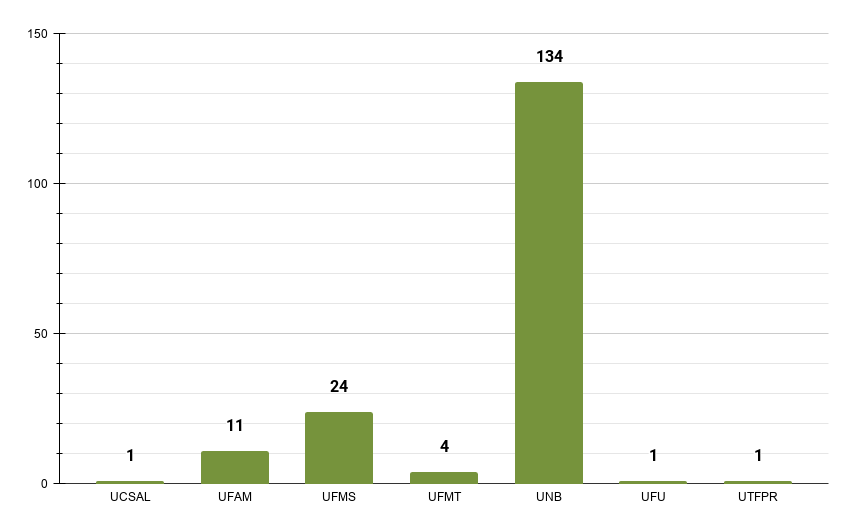
\includegraphics[keepaspectratio=true,scale=0.5]{figuras/apendice/graficos_survey/campus.png}
	\label{Fig:campus.png}
\end{figure}

Em relação aos respondentes e o curso de Interação Humano-Computador, foi observado que 54 respondentes não haviam feito a disciplina, 30,7\% do total; 57 já haviam feito a disciplina, 32,4\% do total; e 65 estavam fazendo a disciplina durante esta pesquisa, 36,9\% do total. Adiante, a Figura \ref{Fig:curso.png}, da relação dos respondentes e o curso de IHC.

\begin{figure}[htbp]
	\centering
	\caption{Relação do respondente com o curso de IHC}
	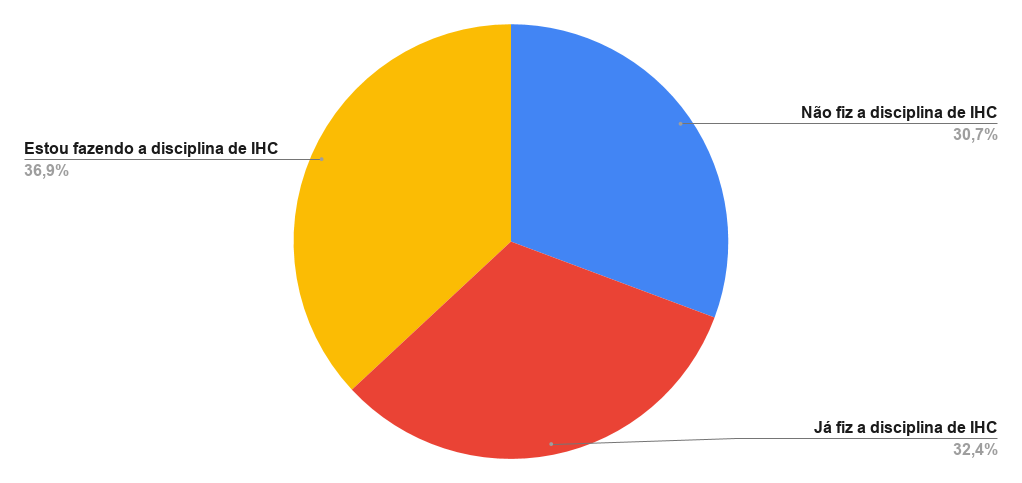
\includegraphics[keepaspectratio=true,scale=0.4]{figuras/apendice/graficos_survey/curso.png}
	\label{Fig:curso.png}
\end{figure}
    
\chapter{Relatório de Execução e Resultados da Construção as Pesonas}
\label{ap:persona}

\section{Processo de Construção}

A partir dos perfis dos respondentes do questionário de pesquisa do \textit{Survey} foi possível definir o elenco de personas deste projeto. Na Figura \ref{Fig:process_persona.png} a seguir é demonstrada uma visão geral das etapas para a definição das personas.

\begin{figure}[htbp]
	\centering
	\caption{Processo de Construção das personas}
	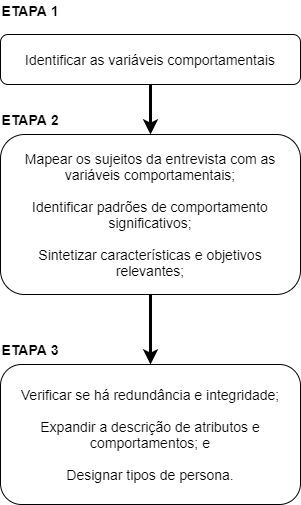
\includegraphics[keepaspectratio=true,scale=0.8]{figuras/personas/process_persona.png}
	\label{Fig:process_persona.png}
\end{figure}

Na primeira etapa foram identificadas as variáveis comportamentais. Estas foram se originaram do próprio questionário de pesquisa. Seguem as variáveis:

\begin{itemize}
    \item I04: pode evidenciar um certo grau de conhecimento mais técnico entre os usuários que cursam graduação na área de Ciência da Computação e os de outros cursos;
    \item O01: pode evidenciar um certo grau de conhecimento e experiência do usuário em relação a área de Interação Humano-Computador;
    \item H01: pode evidenciar um certo grau de conhecimento e experiência mais prática em IHC;
    \item H02: pode evidenciar um certo grau de conhecimento e experiência mais prática em IHC;
    \item RL01: ajuda a identificar os relacionamentos mais relevantes do usuário no contexto de ensino e aprendizagem, que serve para identificar uma oportunidade de intervenção em que um jogo educacional pode auxiliar nessas relações;
    \item O02: quesito base que evidencia o nível de afinidade do usuário com jogos educacionais;
    \item O02.1.1, O02.2.1 e O02.3.1: quesito que evidencia o objetivo do usuário ao usar um jogo educacional;
    \item O02.1.2 e O02.2.2: auxilia na percepção da frequência em que os usuários costumam usar jogos educacionais;
    \item O02.1.4: auxilia na identificação de usuários específicos que têm uma afinidade relevante para com os jogos educacionais; 
    \item O02.3.2 e O02.4.1: auxilia na complementação das características das anti-personas
    \item RE01 e E01: serve para identificar a preferencia dos usuários em relação às características e experiências dos jogos educacionais;
\end{itemize}

Após a identificação das variáveis comportamentais o processo seguiu para a etapa de mapeamento dos respondentes em relação a essas variáveis, a identificação de padrões de comportamento significativos e a sintetização de características e objetivos relevantes. Essas três etapas foram executadas de forma simultânea até ser possível ter as estruturas base das personas. 

Como as respostas do questionário foram armazenadas em uma planilha eletrônica (PE0), foi feito o uso desta ferramenta nesse processo de filtragem e sintetização dos dados. Primeiramente foram separados em duas planilhas os dados dos respondentes a partir da variável I04, definindo então a base da caracterização da anti-persona (PE2) e das demais personas (PE1). Na Figura \ref{Fig:persona_tree.png} é apresentada o processo da evolução das planilhas geradas para a construção das personas, que é descrita logo após.

\begin{figure}[htbp]
	\centering
	\caption{Fluxo do processo de construção das personas}
	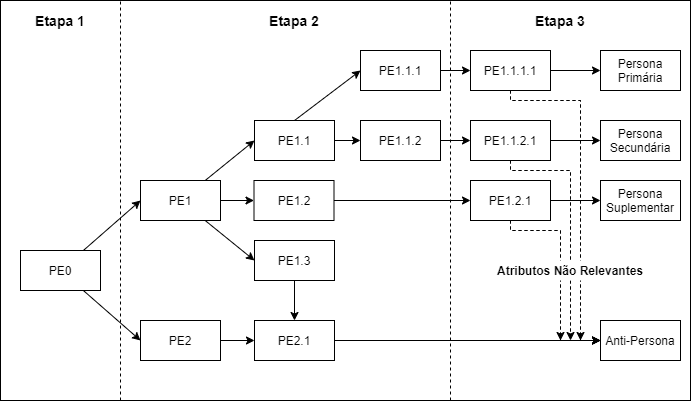
\includegraphics[keepaspectratio=true,scale=0.6]{figuras/personas/persona_tree.png}
	\label{Fig:persona_tree.png}
\end{figure}

A partir da variável O02 foi possível filtrar os respondentes. O resultado foi, perfis que responderam que usam jogos e perfis que já usaram, mas não usam mais (PE1.1), perfis que responderam que nunca jogaram, mas tinham um interesse (PE1.2) e perfis que não tinham interesse de jogar (PE1.3), que no caso foram englobados ao PE2, formando o PE2.1.

Dentro de PE1.1 existiam aqueles que haviam jogado, mas por algum motivo tinham parado de usar jogos educacionais, destes foram relevantes apenas aqueles que pararam de jogar por terem alcançado seu objetivo por meio do jogo. Foi obtido então PE1.1.1, com os perfis que jogam jogos educacionais e PE1.1.2, com aqueles que haviam jogado, mas pararam por haverem alcançado seu objetivo, estes foram identificados pela variável O02.1.4.

O próximo passo foi observar, a partir das variáveis H01, H02 e O01, quais os perfis seriam mais relevantes. Foi definido então os perfis na PE1.2.1, PE1.1.1.1 e PE1.1.2.1, cujo conhecimento sobre IHC era bem básico ou nenhum, sendo que estas ou estavam fazendo o curso de IHC ou ainda não haviam feito.

Tendo sido agrupados e filtrados esses conjuntos de características foi possível identificar os objetivos (O02.1.1, O02.2.1 e O02.3.1) dos jogadores que merecem destaque e quais suas preferências de experiência e elementos de jogos (RE01 e E01). 

Traçados esse esboço inicial das personas, foram realizadas as últimas etapas. Foi verificada a integridade das personas e se haviam redundâncias, uma descrição mais detalhada de atributos e comportamentos foram inseridos tirando como base algumas variáveis comportamentais (RL01, O02.1.2 e O02.2.2) e outras variáveis de identificação (I01, I02 e I03). Por fim foram designados os tipos de personas, primária, secundária e suplementar. No caso da anti-personas, as variáveis O02.3.2 e O02.4.1 auxiliaram a complementar suas características.

\section{Personas do Projeto}
A seguir encontram-se as personas construídas para esse projeto. A persona primária, Victor Matheus Farias; a persona secundária, Afonso Souza de Queiroz; a persona suplementar, Natália Figueiredo; e a anti-persona, Rafael Medeiros.

\begin{table}[htbp]
\centering
\caption{Persona Primária}
\label{tab:Table_persona1}
\small
\begin{tabular}{| m{0.25\textwidth} m{0.65\textwidth}|}
\hline \multicolumn{2}{|c|}{\textbf{Identidade}} \\ \hline
& \\

\begin{center} 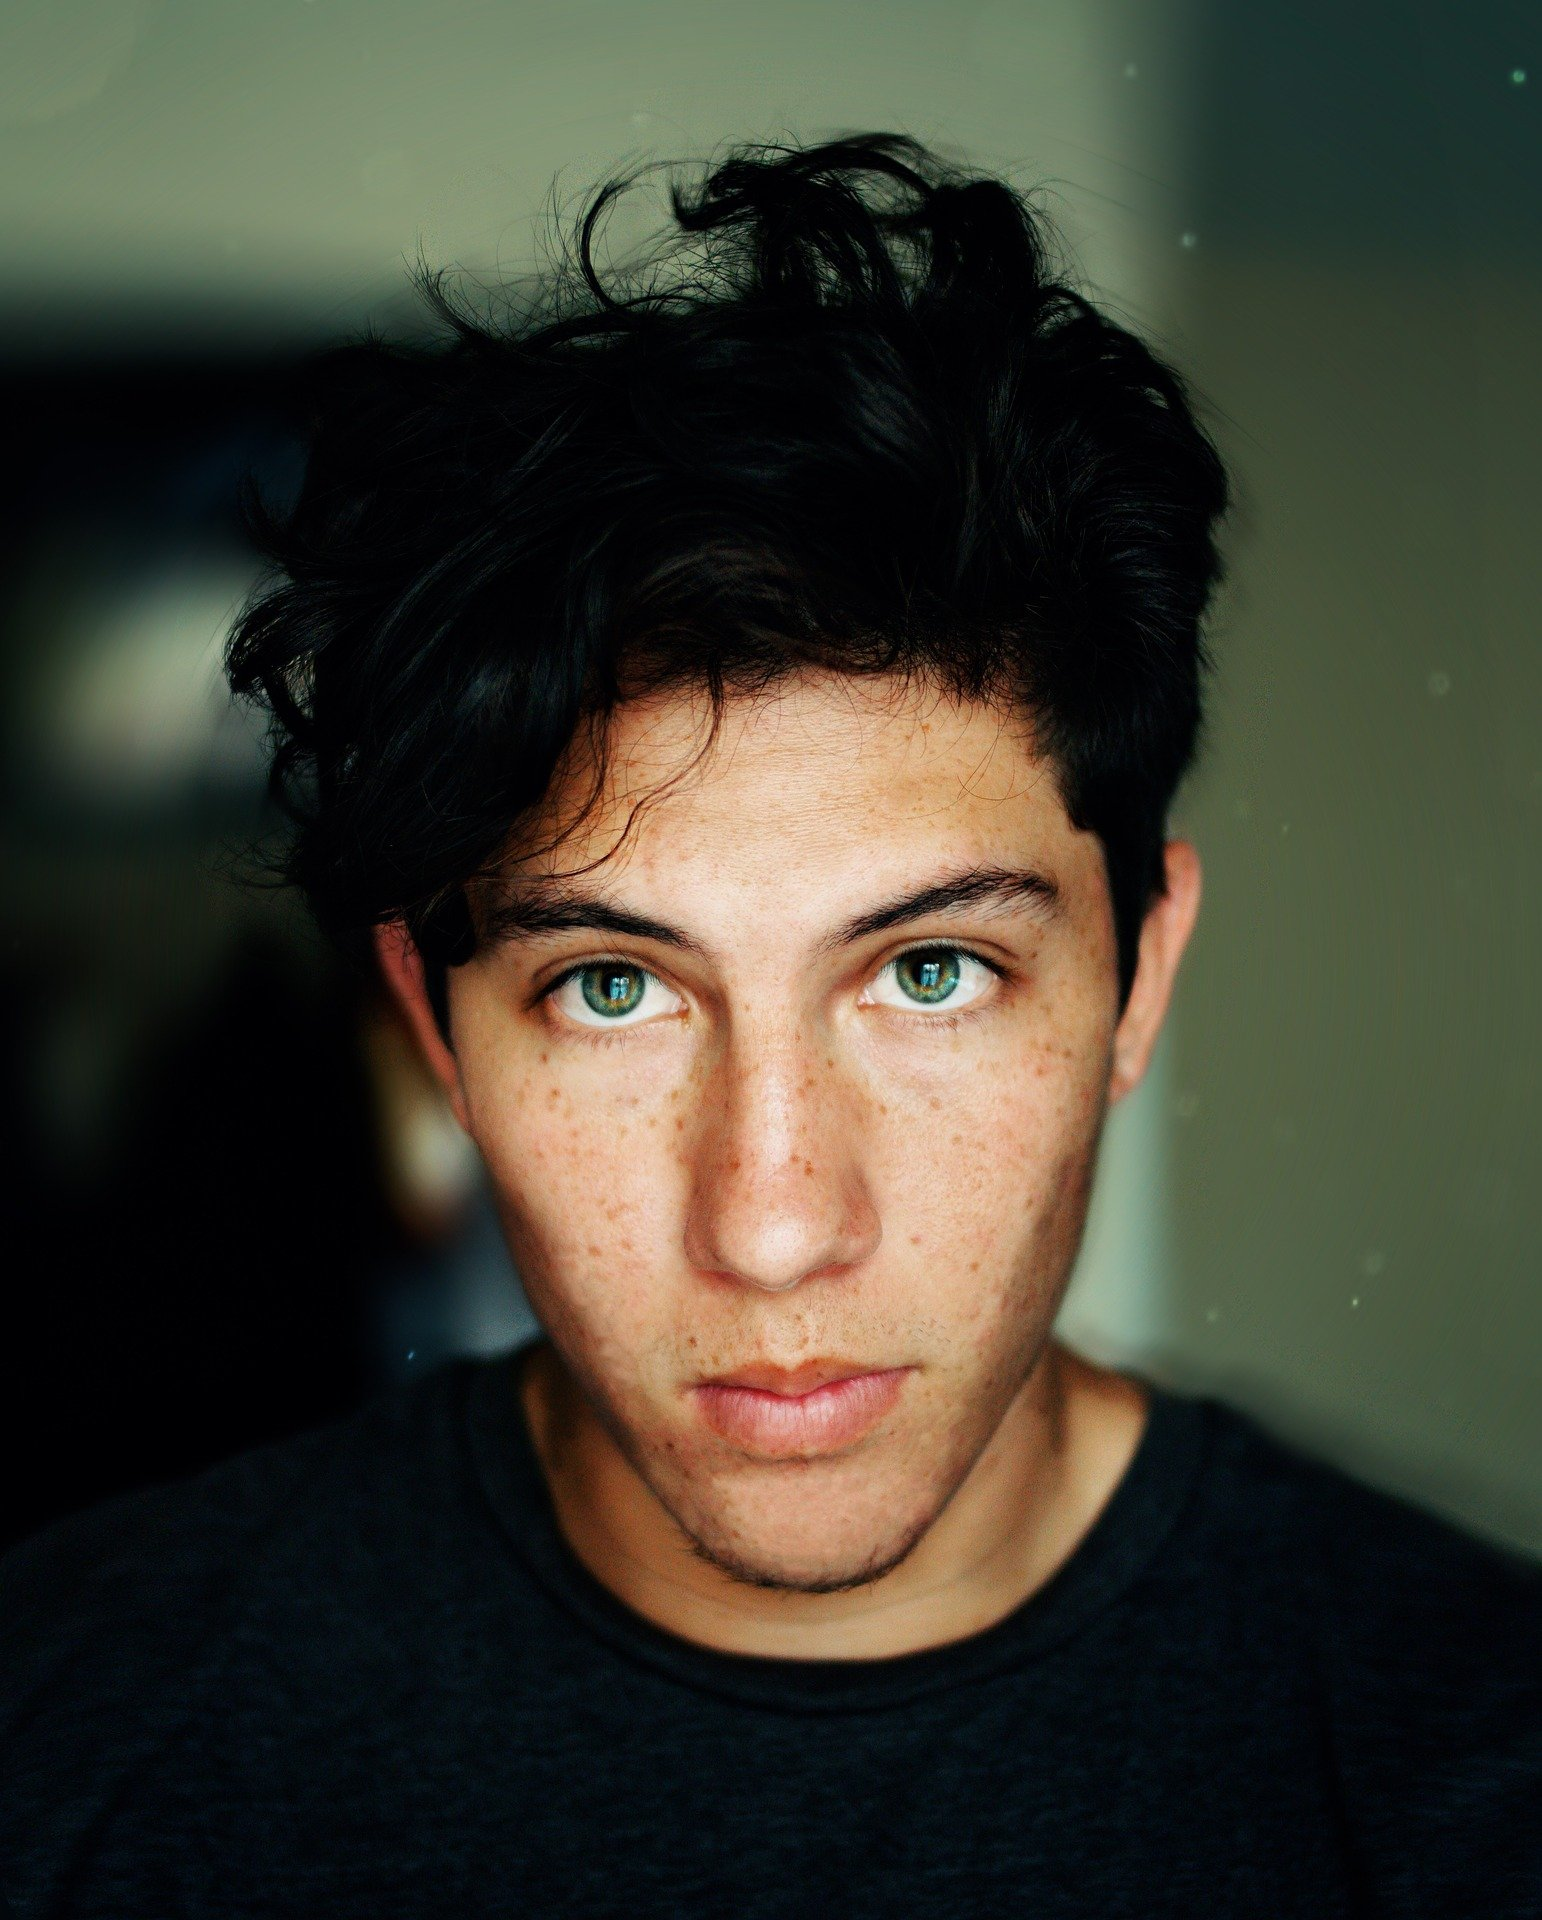
\includegraphics[scale=0.06]{figuras/personas/portrait-3353699_1920.jpg} \end{center} 

&

\textbf{Nome: } Victor Matheus Farias

\textbf{Idade:} 19 anos

\textbf{Ocupação:} Estudante de Engenharia de Software na UnB, Faculdade do Gama.

\\ \hline


\multicolumn{2}{|c|}{\textbf{Descrição}} \\ \hline
\multicolumn{2}{|p{15cm}|}{
        Aprender algum conteúdo novo é meu o principal objetivo ao usar jogos educacionais. Atualmente eu uso alguns jogos educacionais, mas com uma frequência moderada. Vejo-os como ferramentas que me auxiliam no processo de aprendizagem. Estou cursando a disciplina de IHC e não tenho muito conhecimento em relação a elaboração de design de interfaces e o pouco que tenho está somente no âmbito disciplinar, daquilo que já vi na disciplina. Desejaria utilizar um jogo que me ajudasse a aprender o conteúdo.
       
        Geralmente quando vou estudar ou sanar alguma dúvida que tenho sobre o conteúdo eu recorro primeiramente à artigos da internet. Em alguns casos assisto vídeo aulas e também utilizo do material disponibilizado pelo professor.
        
        Outros meios que uso para sanar as dúvidas que tenho em relação ao conteúdo é perguntar a colegas que já fizeram a disciplina e também geralmente estudo com colegas que estão fazendo a disciplina comigo. Busco em alguns casos tirar as dúvidas com os monitores ou professor.
        Os requisitos do jogo que me levam a usá-lo são: 
        \begin{itemize}
            \item um design atraente e consistente; 
            \item o jogo ser fácil de aprender a jogar e fácil de se jogar, com regras claras; 
            \item um bom uso de fontes e cores; 
            \item que o jogo ofereçam feedbacks relevantes. 
        \end{itemize}
        
        Ao usar um jogo eu espero ter certeza que vou  aprender o conteúdo ali apresentado, espero que seja algo desafiador, divertido e satisfatório aprender jogando. 
        
        Jogos que prendem minha atenção e me envolvem para aprender o conteúdo são bem relevantes, ainda mais se eu conseguir perceber a importância do conteúdo que estou aprendendo.} \\ \hline
\end{tabular}
\end{table}
\begin{table}[htbp]
\centering
\caption{Persona Secundária}
\label{tab:Table_persona2}
\small
\begin{tabular}{| m{0.25\textwidth} m{0.65\textwidth}|}
\hline \multicolumn{2}{|c|}{\textbf{Identidade}} \\ \hline
& \\

\begin{center} 
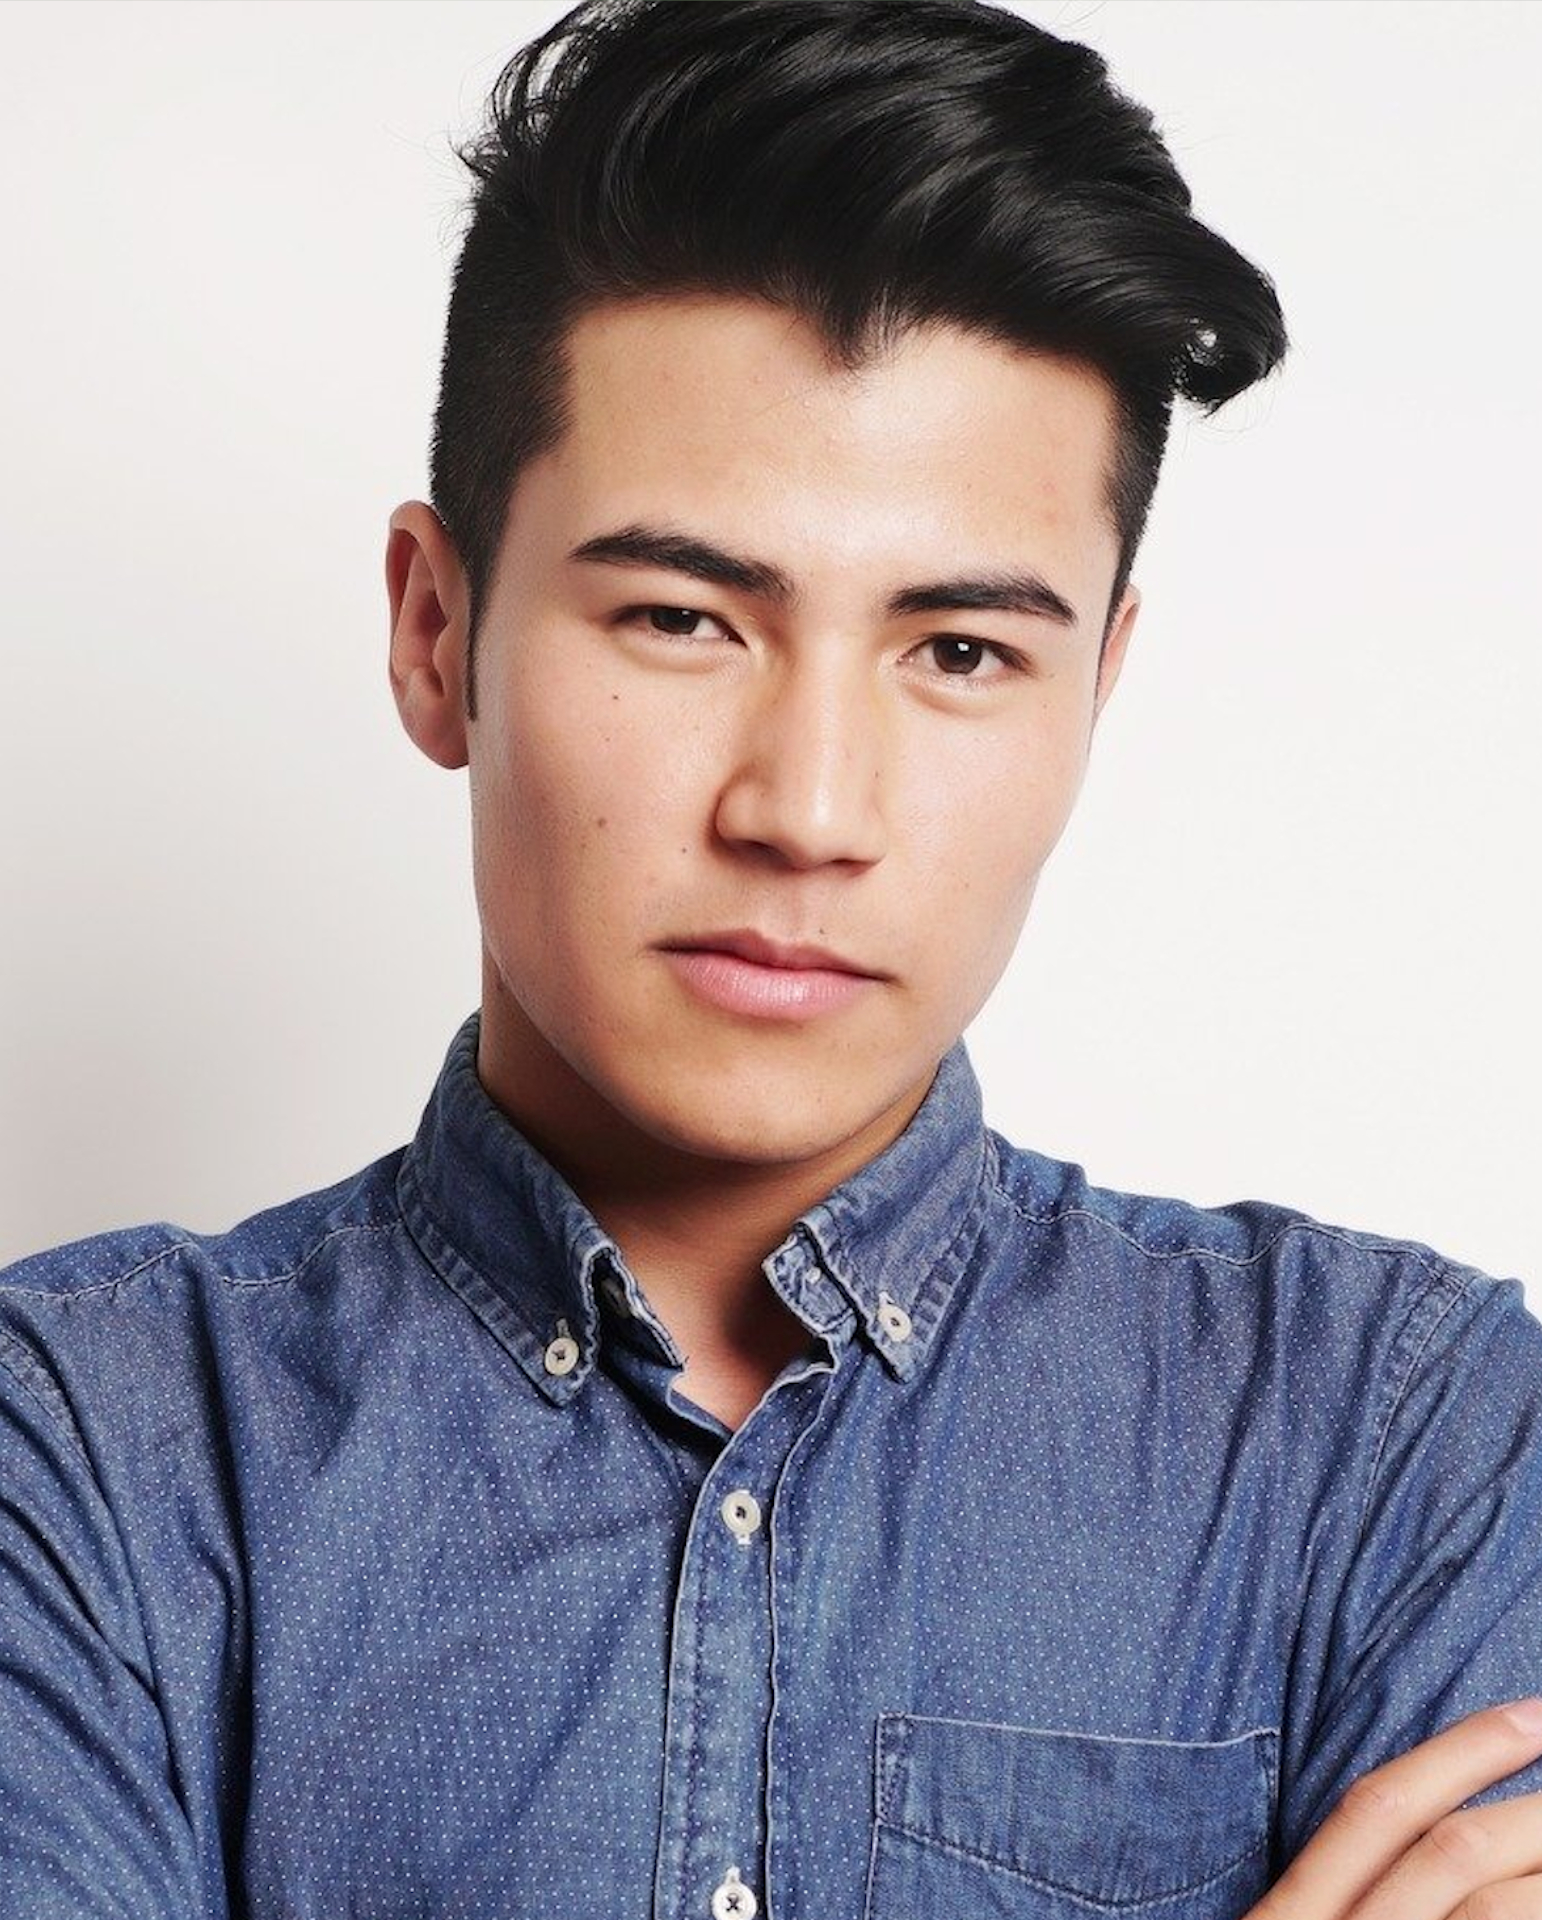
\includegraphics[scale=0.06]{figuras/personas/model-2911332_1920.jpg} 
Fonte: Pixabay\tablefootnote{https://pixabay.com/photos/model-businessman-corporate-2911332/}
\end{center} 

&

\textbf{Nome: } Afonso Souza de Queiroz

\textbf{Idade:} 19 anos

\textbf{Ocupação:} Estudante de Engenharia de Software na UnB, Faculdade do Gama

\\ \hline


\multicolumn{2}{|c|}{\textbf{Descrição}} \\ \hline
\multicolumn{2}{|p{15cm}|}{
     \begin{tabular}[c]{@{}l@{}}\\
        Já joguei alguns jogos educacionais onde meu principal objetivo era aprender um\\ conteúdo novo. Além disso era interessante quando o jogo possibilitava que eu revisasse\\ o conteúdo e avaliasse o que tinha aprendido. Eu jogava com certa moderação. Por mais\\ que atualmente eu não esteja usando algum jogo educacional, eu parei de jogar pois \\alcancei meus objetivos de estudo e me sentiria da mesma forma se houvesse algum\\ jogo que me ajudasse nas matérias da faculdade.\\ 
        \\
        Ainda não fiz a disciplina de IHC, por isso não tenho muito conhecimento em relação\\ a elaboração de design de interfaces, sendo que o pouco que tenho veio de projetos de\\ outras disciplinas e atividades extra curriculares.\\
        \\
        Gosto mais de estudar sozinho, pesquisando na internet e indo por conta própria atrás\\ de materiais de estudo. Apenas quando não acho nada relevante, recorro aos materiais\\ disponibilizados pelo professor.\\
        \\
        Para mim, um jogo onde vou aprender deve ter um design com um \textbf{padrão simples},\\ mas que desperte \textbf{interesse}; deve me dar bons \textbf{feedbacks} a cada interação que faço\\ no jogo; deve ser algo \textbf{simples de aprender como jogar} e \textbf{simples de jogar}; e caso\\ tenha textos sobre o conteúdo, seria bom que os textos fossem bem objetivos e com\\ uma cor e fonte que facilitasse a leitura.\\ 
        \\
        Espero ter a sensação logo de cara que \textbf{não vou perder meu tempo} com o jogo, mas\\ que ao final vou perceber o quanto foi \textbf{importante aprender o conteúdo} e o quanto\\ foi \textbf{satisfatório} ter me \textbf{divertido} aprendendo. E espero também de certa forma ser\\ \textbf{desafiado}, pois isso me ajuda a \textbf{focar} na atividade que estou realizando.\\ \\ 
    \end{tabular}
} \\ \hline
\end{tabular}
\end{table}
\newpage

\begin{table}[htbp]
\centering
\caption{Persona Suplementar}
\label{tab:Table_persona3}
\small
\begin{tabular}{| m{0.25\textwidth} m{0.65\textwidth}|}
\hline \multicolumn{2}{|c|}{\textbf{Identidade}} \\ \hline
& \\

\begin{center} 
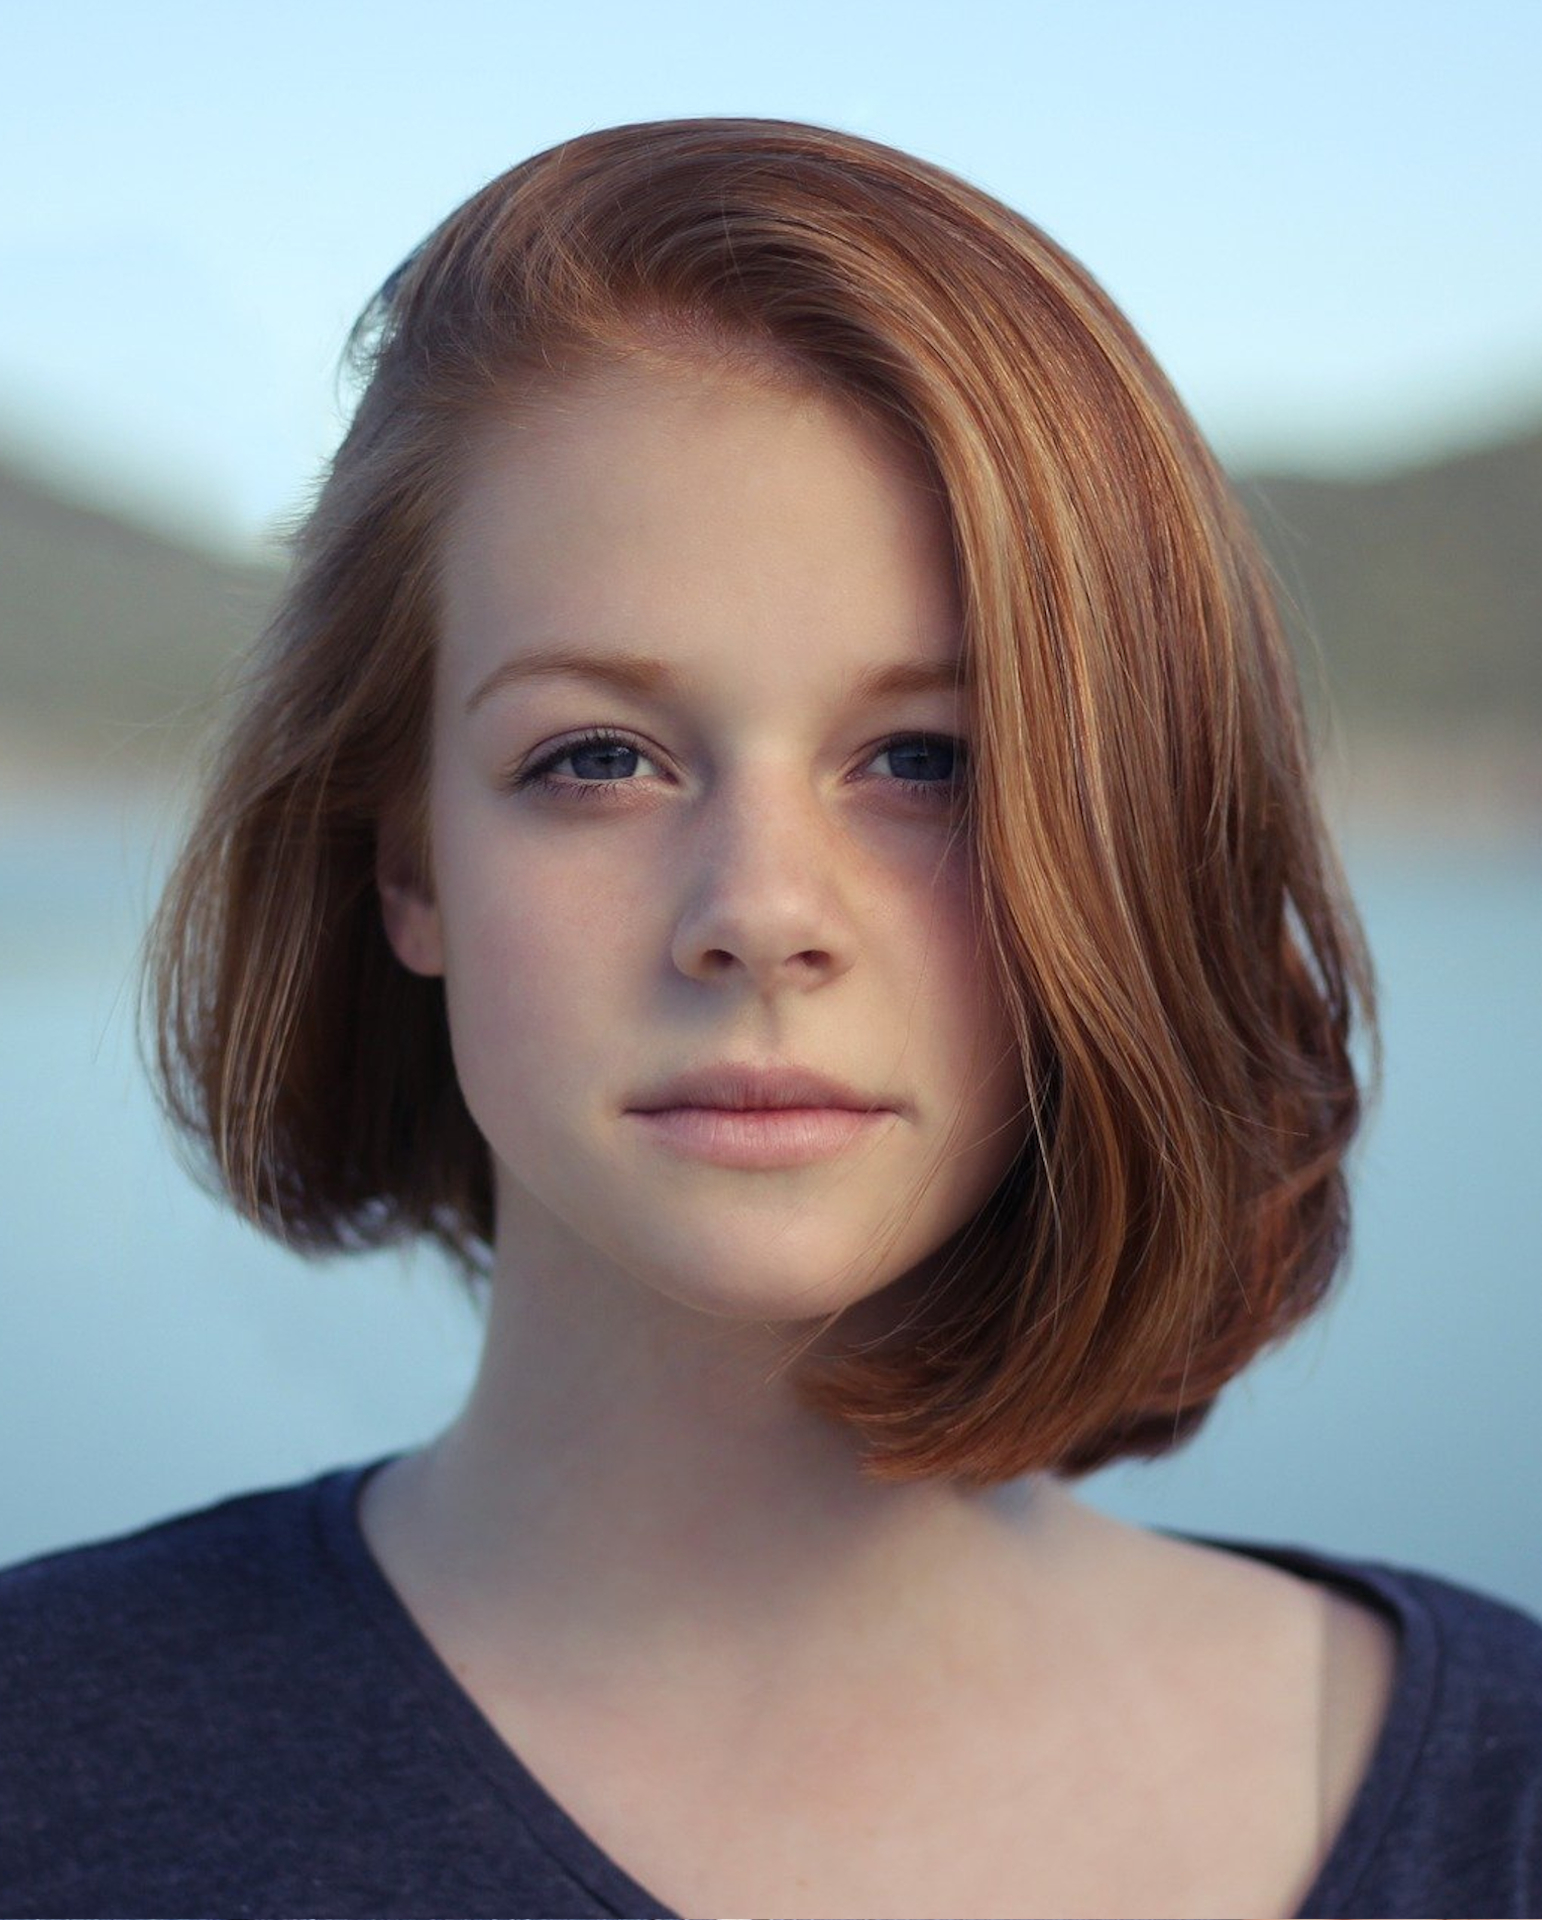
\includegraphics[scale=0.06]{figuras/personas/girl-919048_1920.jpg}
Fonte: Pixabay\tablefootnote{https://pixabay.com/photos/girl-portrait-hairstyle-redhead-919048/}
\end{center} 

&

\textbf{Nome: }  Natália Figueiredo

\textbf{Idade:} 23 anos

\textbf{Ocupação:} Estudante de Engenharia de Software na UnB, Faculdade do Gama.

\\ \hline


\multicolumn{2}{|c|}{\textbf{Descrição}} \\ \hline
\multicolumn{2}{|p{15cm}|}{
    \begin{tabular}[c]{@{}l@{}}\\
        Nunca joguei jogos educacionais, pois não conheci nenhum que tinha o propósito de\\ ensinar o que eu desejava. No caso se eu encontrasse um jogo o qual eu pudesse aprender\\ um conteúdo novo e pudesse revisá-lo quando necessário seria interessante. Estou fazendo\\ a disciplina de IHC e desejaria utilizar um jogo que me ajudasse a aprender o conteúdo,\\ pois não tenho muito conhecimento em relação a elaboração de design de interfaces e o\\ pouco que tenho foi somente a partir da disciplina de IHC.\\
        \\
        Geralmente quando vou estudar ou sanar alguma dúvida que tenho sobre o conteúdo eu\\ pesquiso na internet. Em ocasiões bem específicas eu assisto vídeo aulas e também\\ utilizo do material disponibilizado pelo professor. \\
        \\
        Acho que um jogo para se estudar teria de ter um \textbf{design simples}, uma lógica de jogo e\\ \textbf{regras fáceis} de se lembrar. O jogo não deveria ser muito \textbf{difícil}, sendo que o objetivo\\ com ele é aprender. Talvez \textbf{recompensas} e \textbf{mensagens} evidenciando meu progresso\\ seriam interessantes.\\
        \\
        Ao jogar, espero encontrar \textbf{desafios} não muito difíceis, mas que despertem minha\\ \textbf{atenção}. Seria bom, perceber logo de início que o jogo traz um \textbf{conteúdo relevante} e \\que vou \textbf{conseguir aprendê-lo}. E por fim não seria nada ruim sentir \textbf{prazer} em \\aprender e ainda me \textbf{divertir}.\\
        \\
    \end{tabular}
} \\ \hline
\end{tabular}
\end{table}
\newpage


\begin{table}[htbp]
\centering
\caption{Anti Persona}
\label{tab:Table_persona4}
\small
\begin{tabular}{| m{0.25\textwidth} m{0.65\textwidth}|}
\hline \multicolumn{2}{|c|}{\textbf{Identidade}} \\ \hline
& \\

\begin{center} 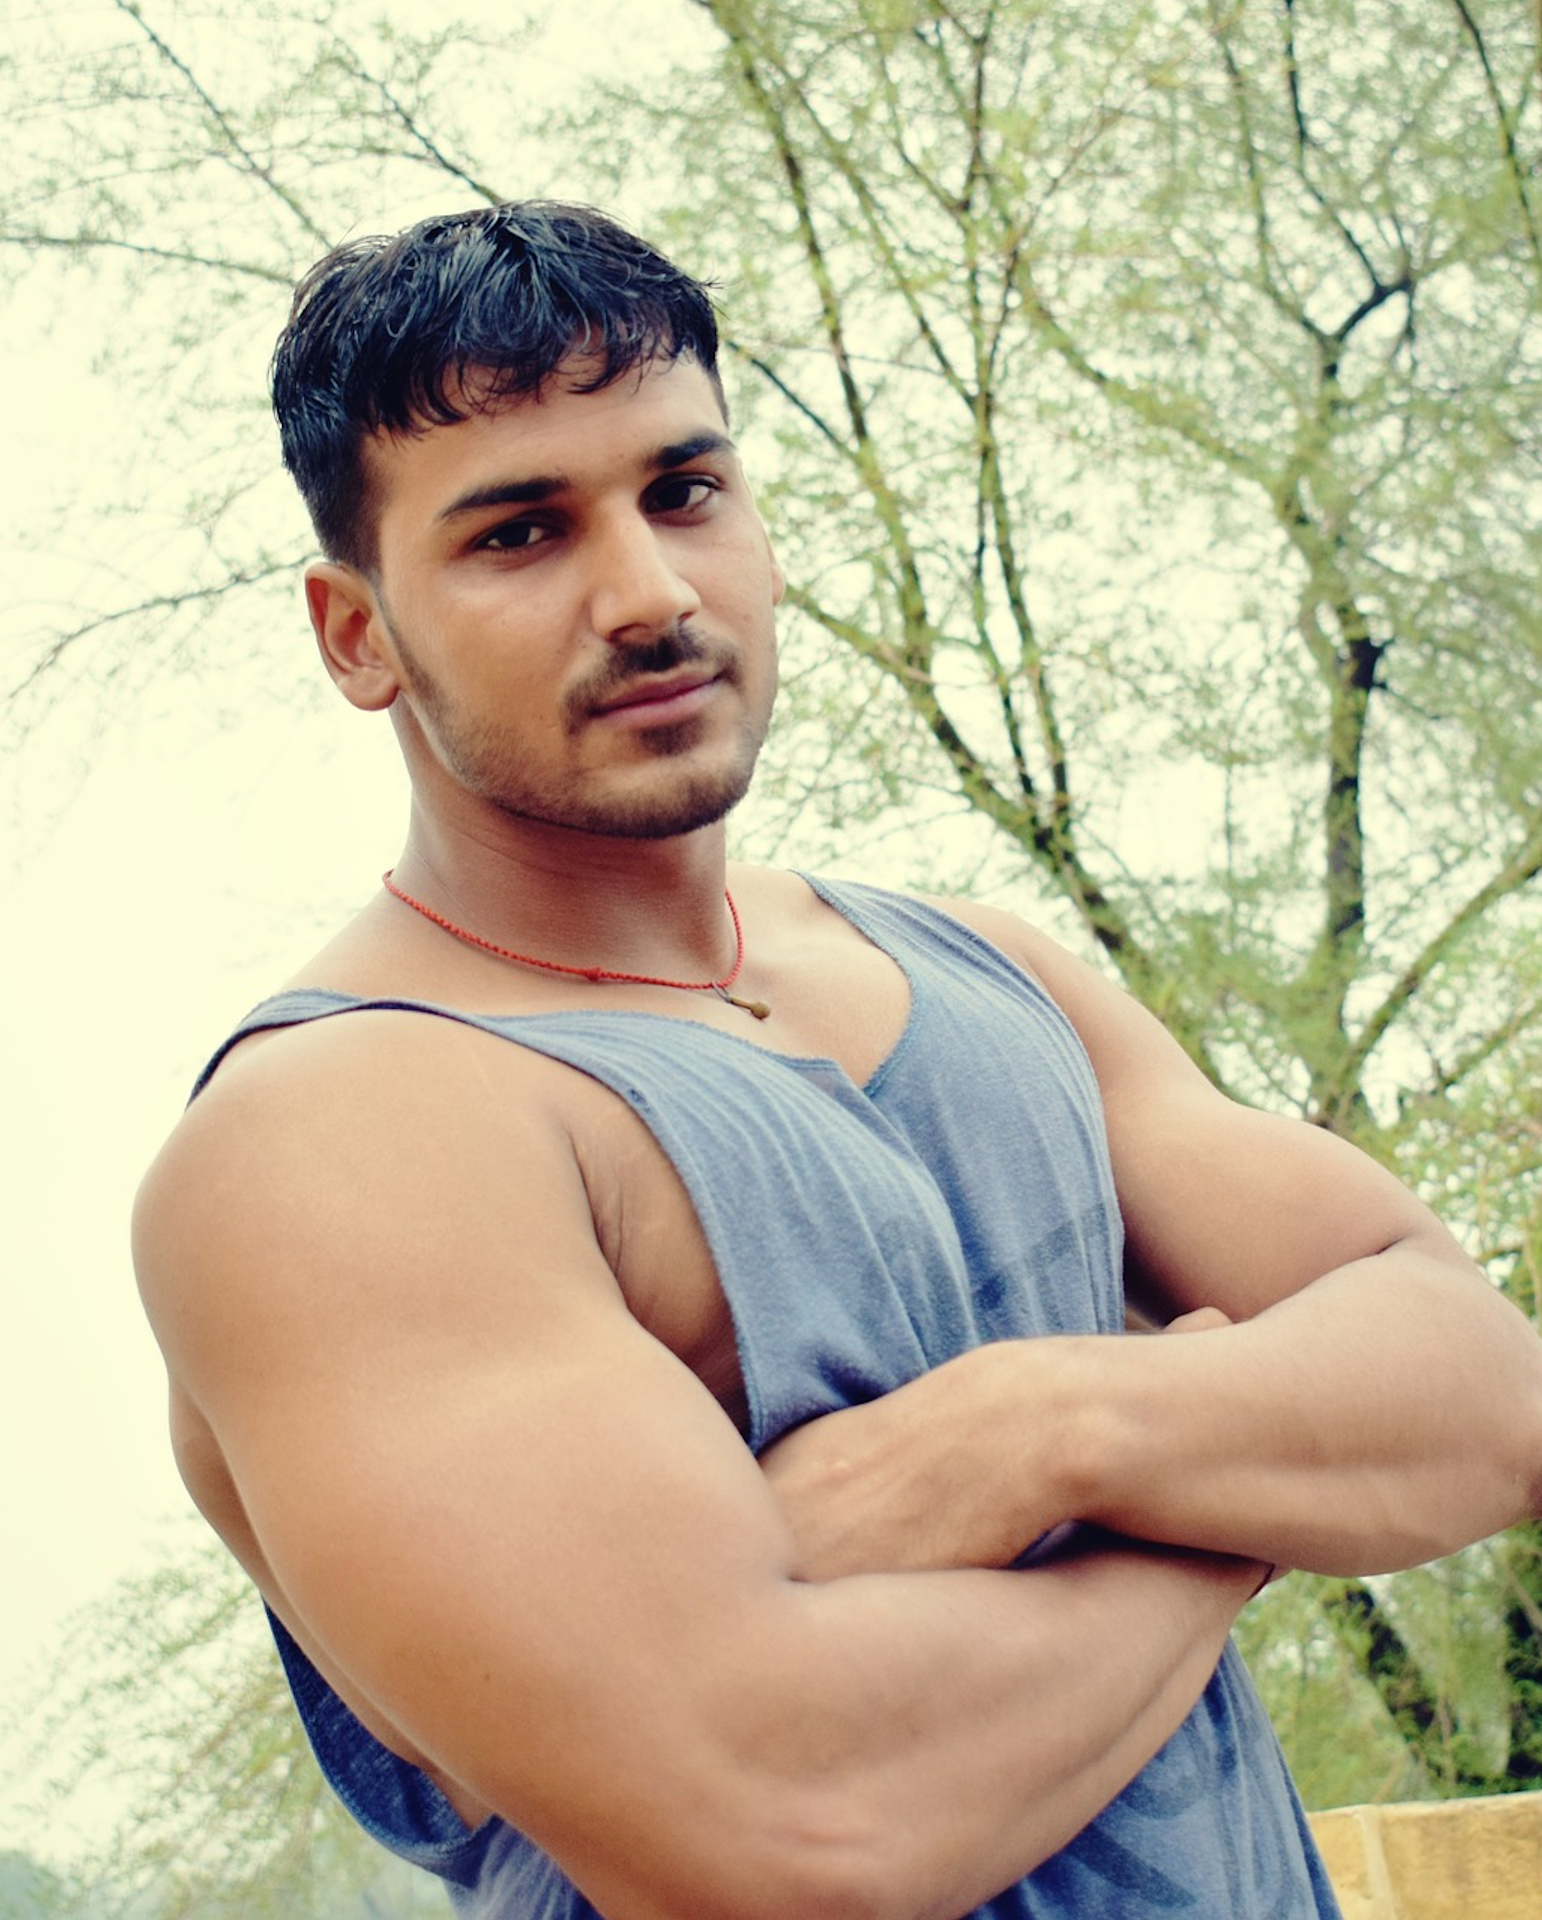
\includegraphics[scale=0.06]{figuras/personas/man-1209494_1920.jpg} \end{center} 

&

\textbf{Nome: }  Rafael Medeiros

\textbf{Idade:} 28 anos

\textbf{Ocupação:} Estudante de Educação Física na UnB, campus Darcy Ribeiro.

\\ \hline


\multicolumn{2}{|c|}{\textbf{Descrição}} \\ \hline
\multicolumn{2}{|p{15cm}|}{
        Não tenho o costume de usar jogos educacionais, devo ter jogado um alguma vez na vida, mas não me interessei muito e rapidamente o jogo se tornou monótono. Gosto de jogar futebol e basquetebol. Em relação ao conhecimento acadêmico, me concentro apenas nas disciplinas do meu curso.
        
        Quando vou estudar ou sanar alguma dúvida que tenho sobre o conteúdo eu utilizo todos os recursos possíveis, priorizando o que for mais prático e objetivo. Geralmente eu tiro dúvidas com colegas que já fizeram a disciplina e colegas que cursam a disciplina comigo. Somente se realmente necessário que vou tirar as dúvidas com os monitores ou professor da matéria. Os requisitos do jogo que me levariam a usá-lo são: 
        
        \begin{itemize}
            \item um design atraente e consistente; 
            \item o jogo ser fácil de aprender a jogar e fácil de se jogar, com regras claras; 
            \item um bom uso de fontes e cores; 
            \item  o jogo ter uma história que me envolvesse seria algo interessante;
            \item que o jogo ofereçam feedbacks relevantes;
            \item pontos e recompensas;
            \item gosto de jogos que promovam interação com outros jogadores, como por exemplo ranking dos jogadores.
        \end{itemize}
        
        Ao usar um jogo eu espero aprender o conteúdo ali apresentado, espero que seja algo desafiador, divertido e satisfatório aprender jogando. Jogos que prendem minha atenção e me envolvem para  aprender o conteúdo são bem relevantes, ainda mais se eu conseguir perceber a importância do conteúdo que estou aprendendo.

       } \\ \hline
\end{tabular}
\end{table}

\chapter{Protótipo de Papel}
\label{ap:proto_papel}

Neste capítulo estão aprestadas as telas do protótipo de baixa fidelidade. Foi usado para isso  a técnica de prototipação em papel.

\begin{figure}[htbp]
	\centering
    \subfigure[Tela de Login]{
        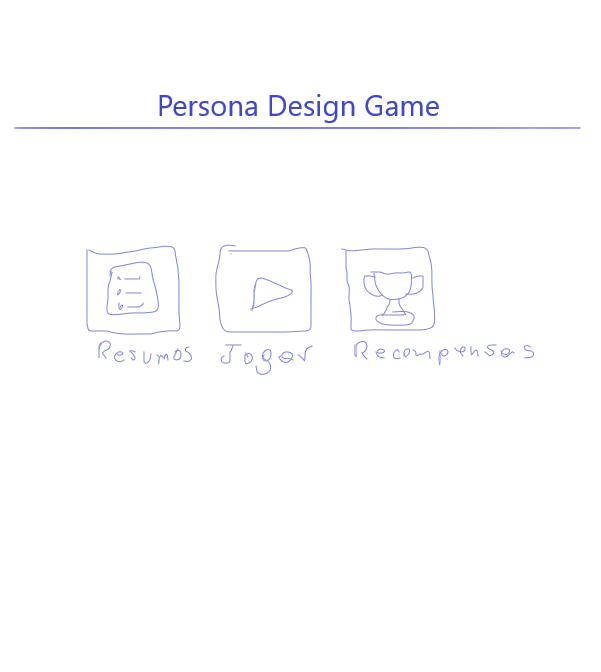
\includegraphics[keepaspectratio=true,scale=0.055]{figuras/prototype/proto1.jpg}
        \label{Fig:login.png}
    }
    \quad
    \subfigure[Tela de Cadastro]{
        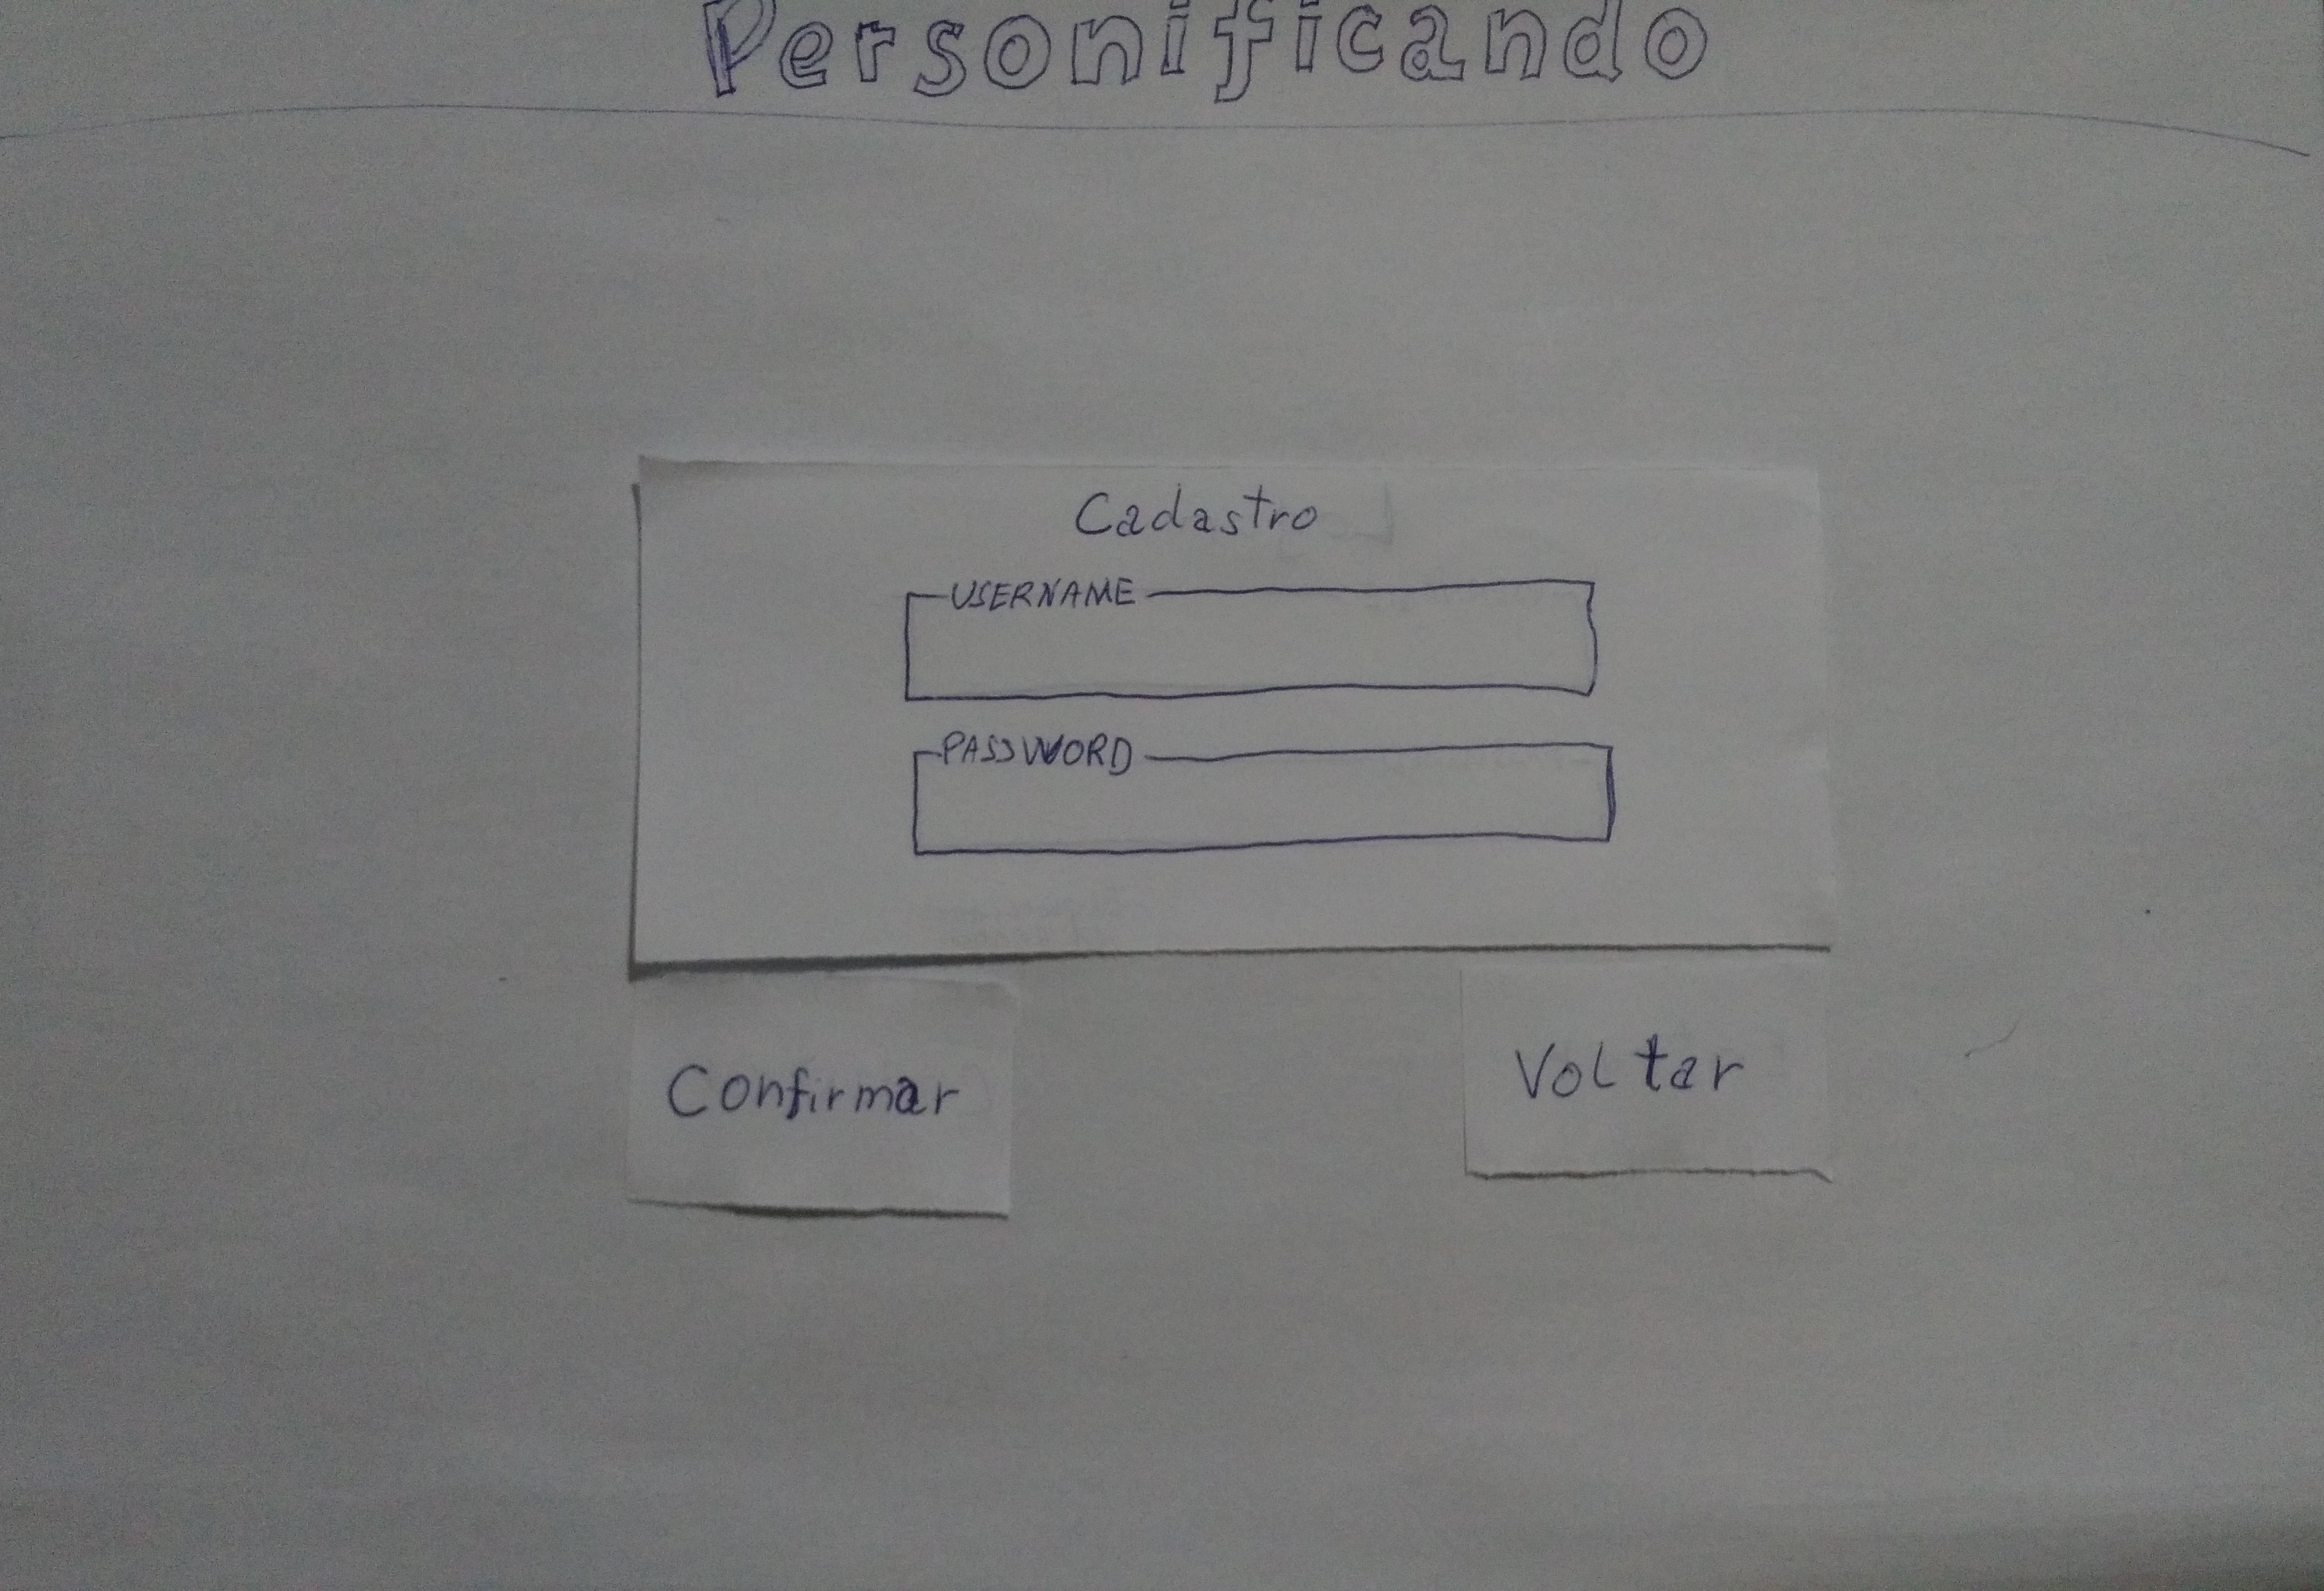
\includegraphics[keepaspectratio=true,scale=0.055]{figuras/prototype/proto2.jpg}
        \label{Fig:cad.png}
    }
    \quad
    \subfigure[Menu Principal]{
        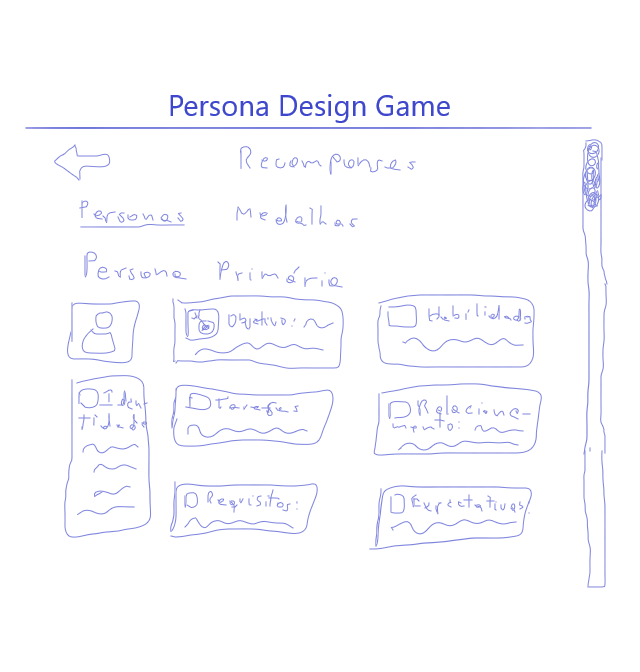
\includegraphics[keepaspectratio=true,scale=0.055]{figuras/prototype/proto3.jpg}
        \label{Fig:menu.png}
    }
    \quad
    \subfigure[Menu Principal - Dropdown Perfil]{
        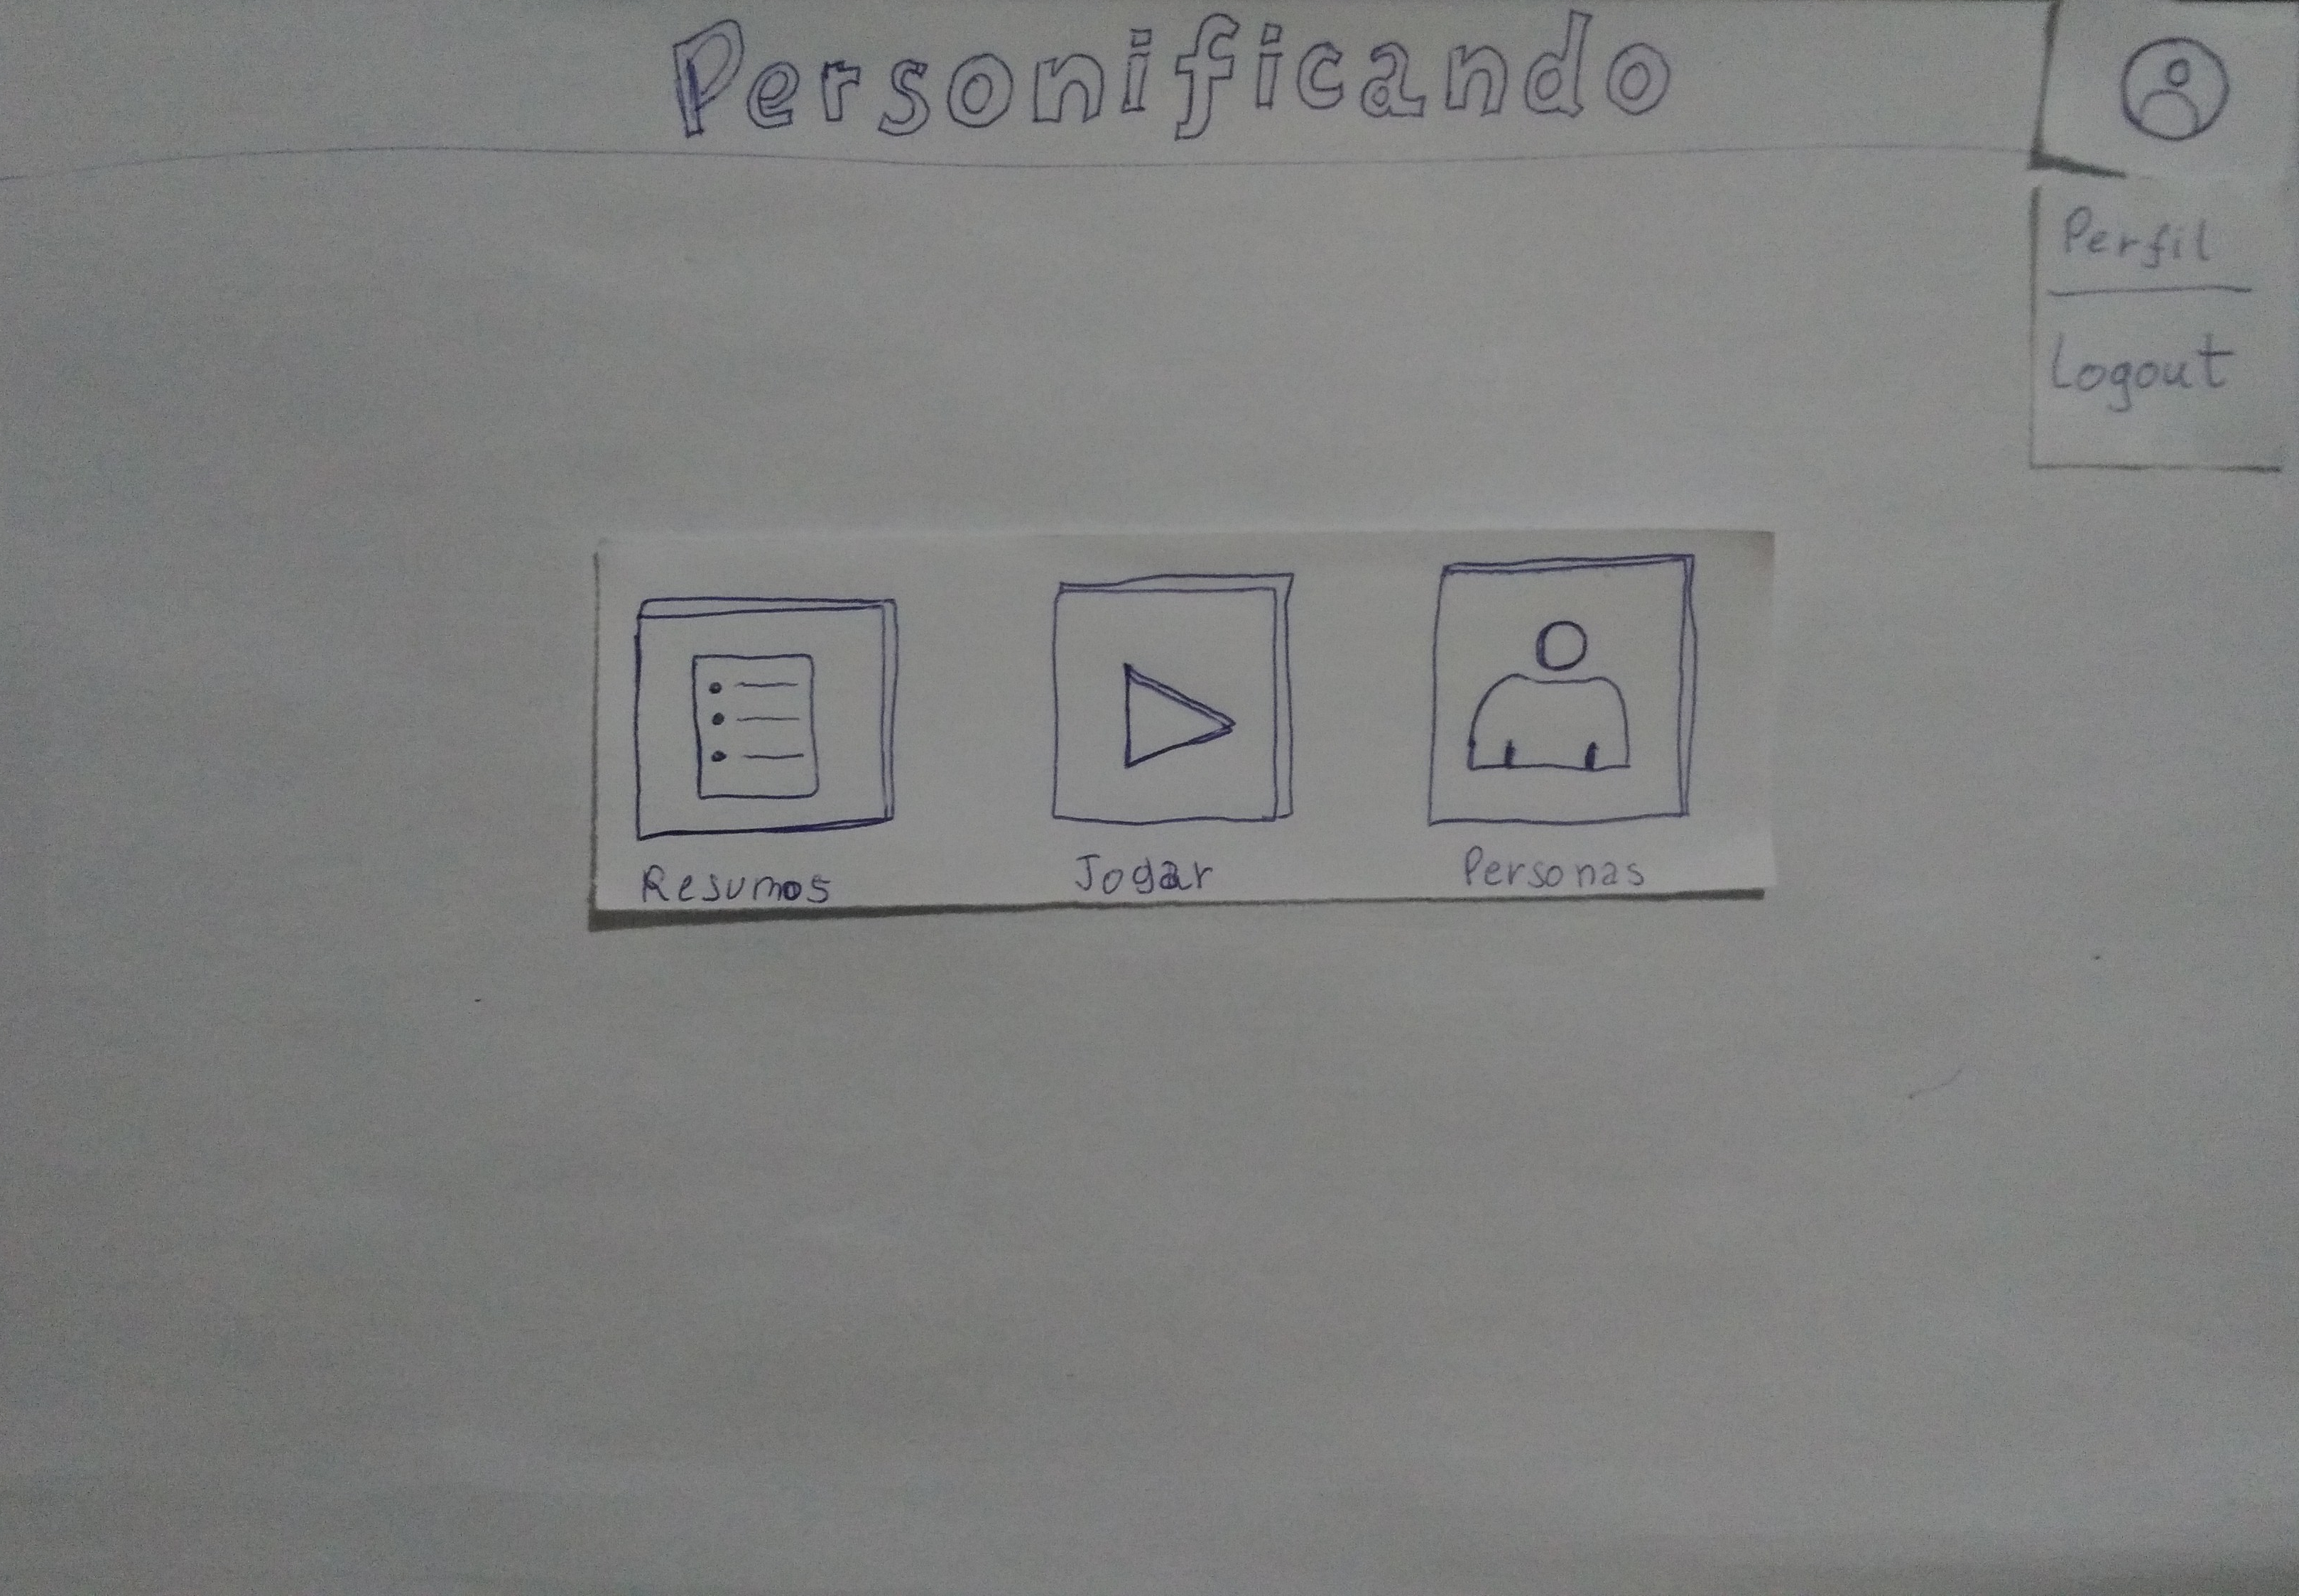
\includegraphics[keepaspectratio=true,scale=0.055]{figuras/prototype/proto4.jpg}
        \label{Fig:menu_drop.png}
    }
    \quad
    \subfigure[Ambiente Resumos]{
        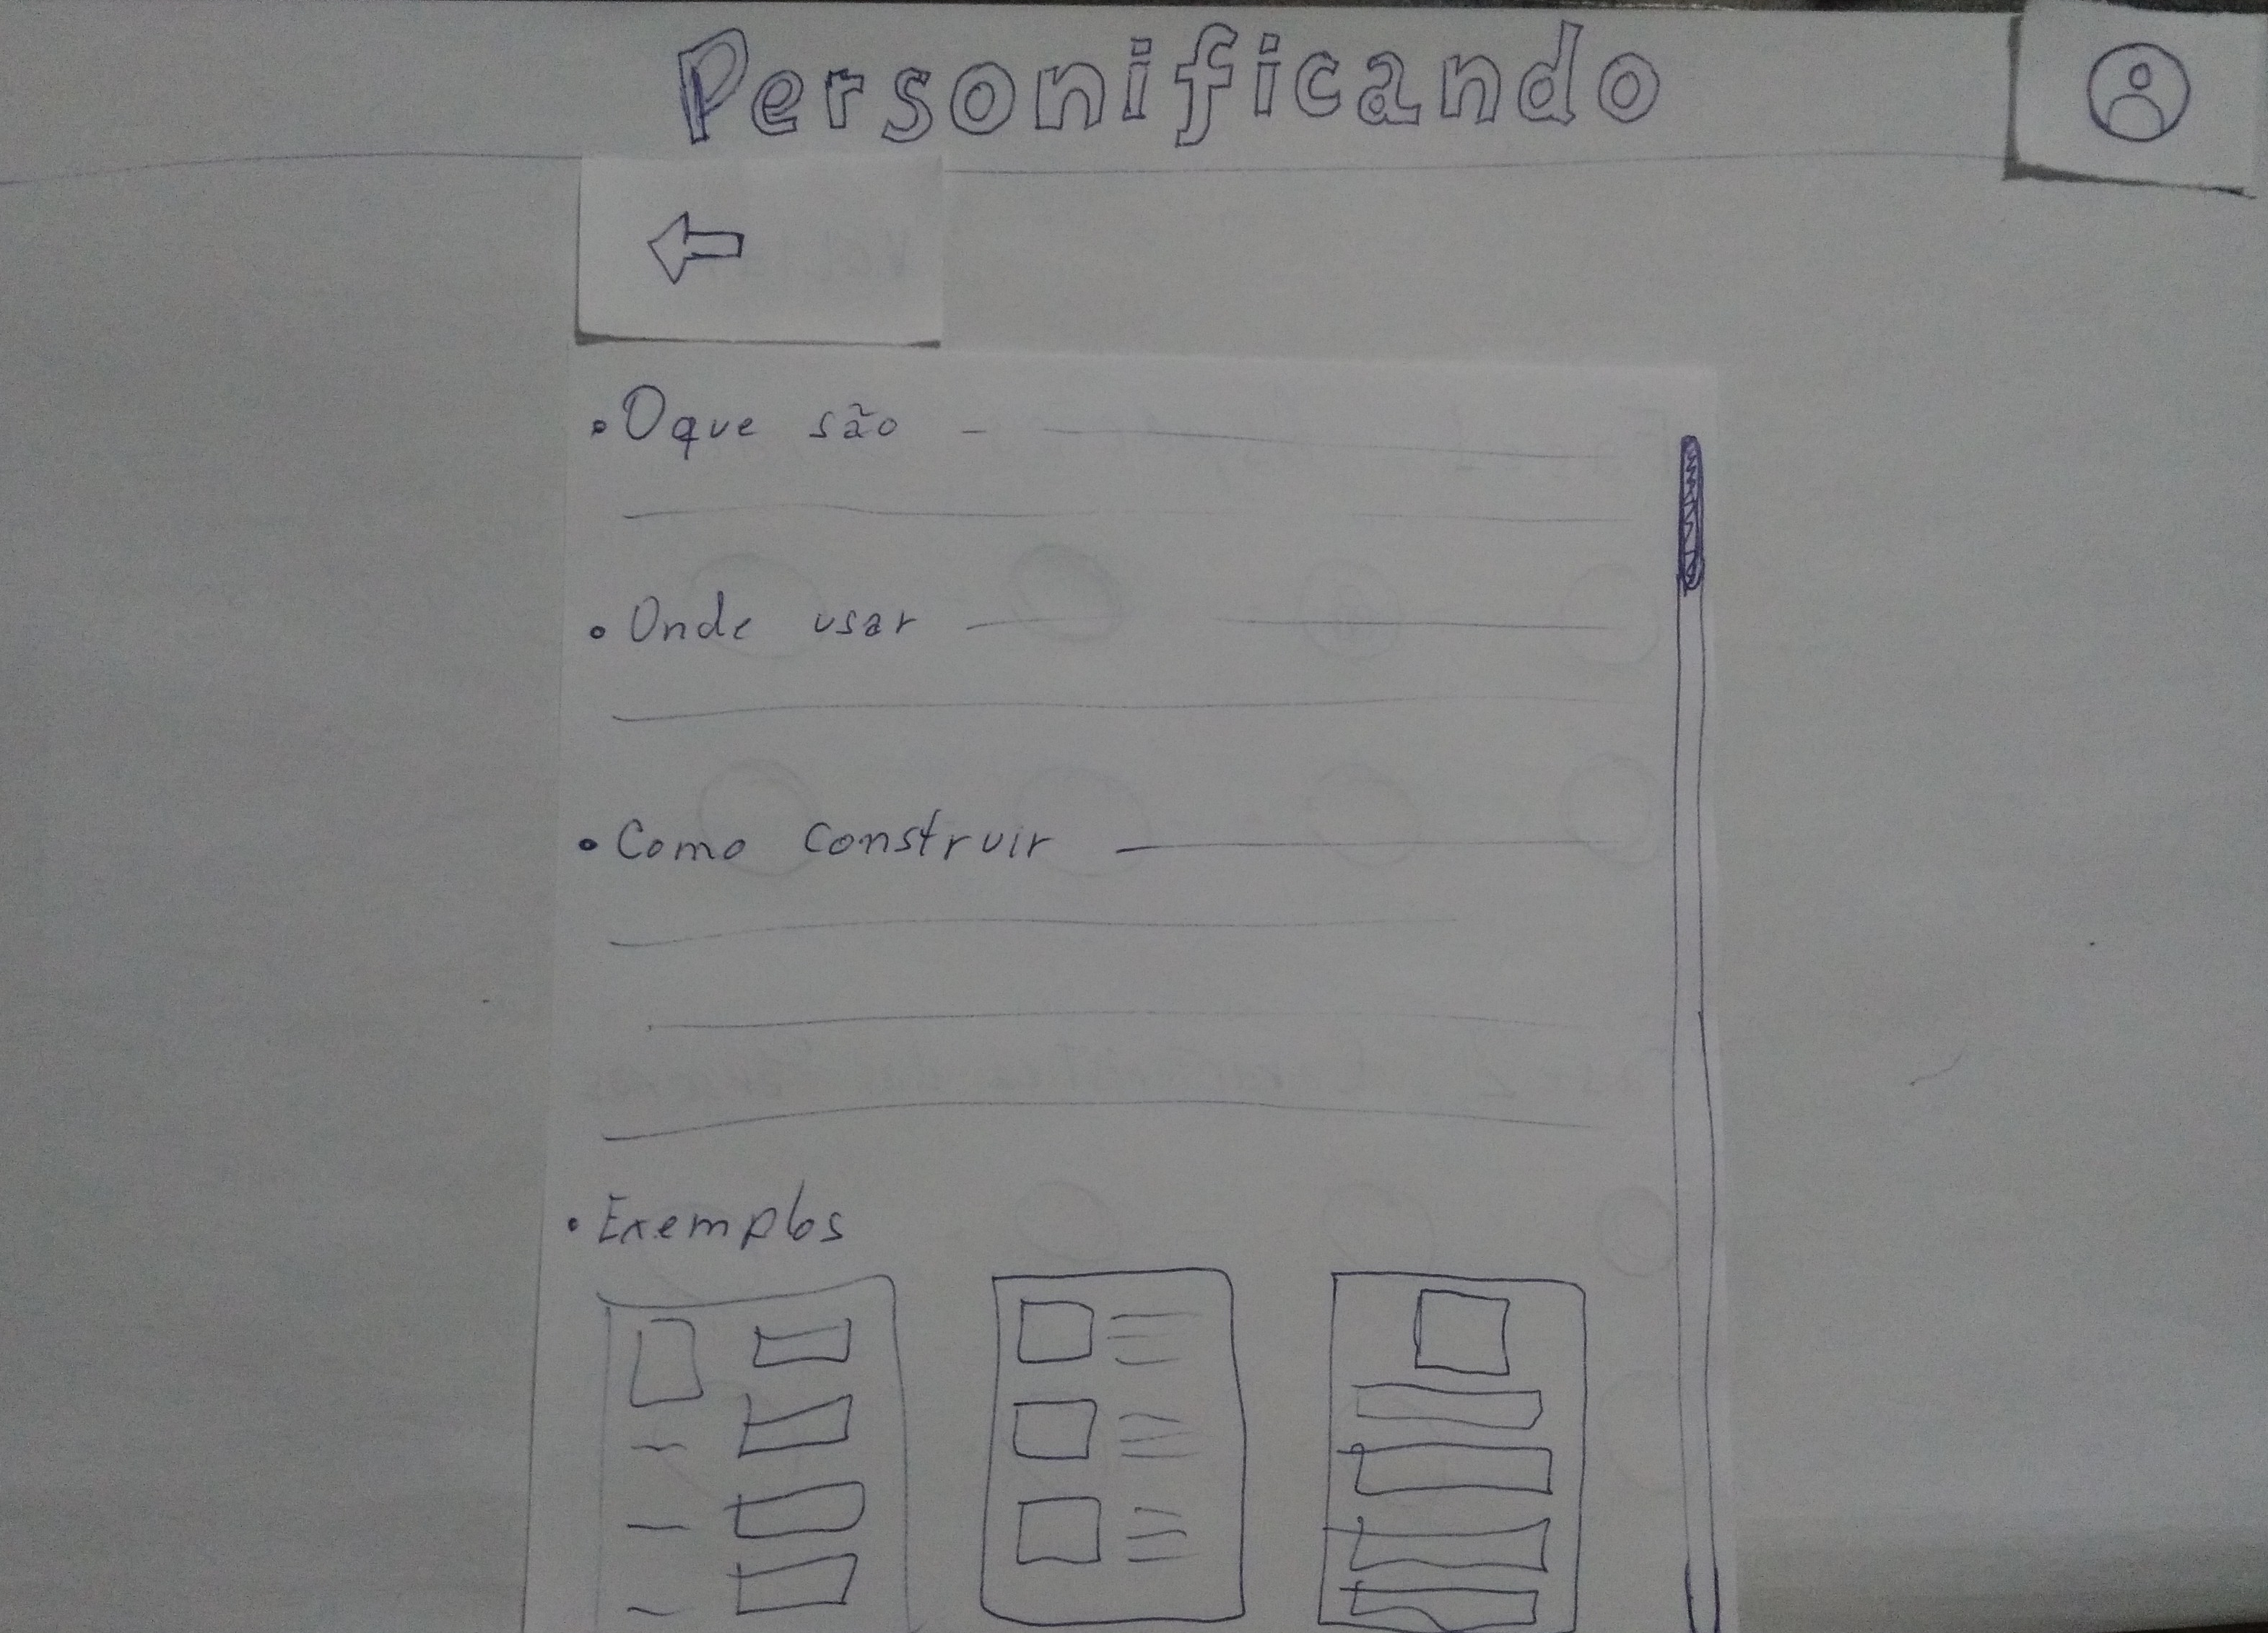
\includegraphics[keepaspectratio=true,scale=0.055]{figuras/prototype/proto5.jpg}
        \label{Fig:amb.png}
    }
    \quad
    \subfigure[Menu das Fases]{
        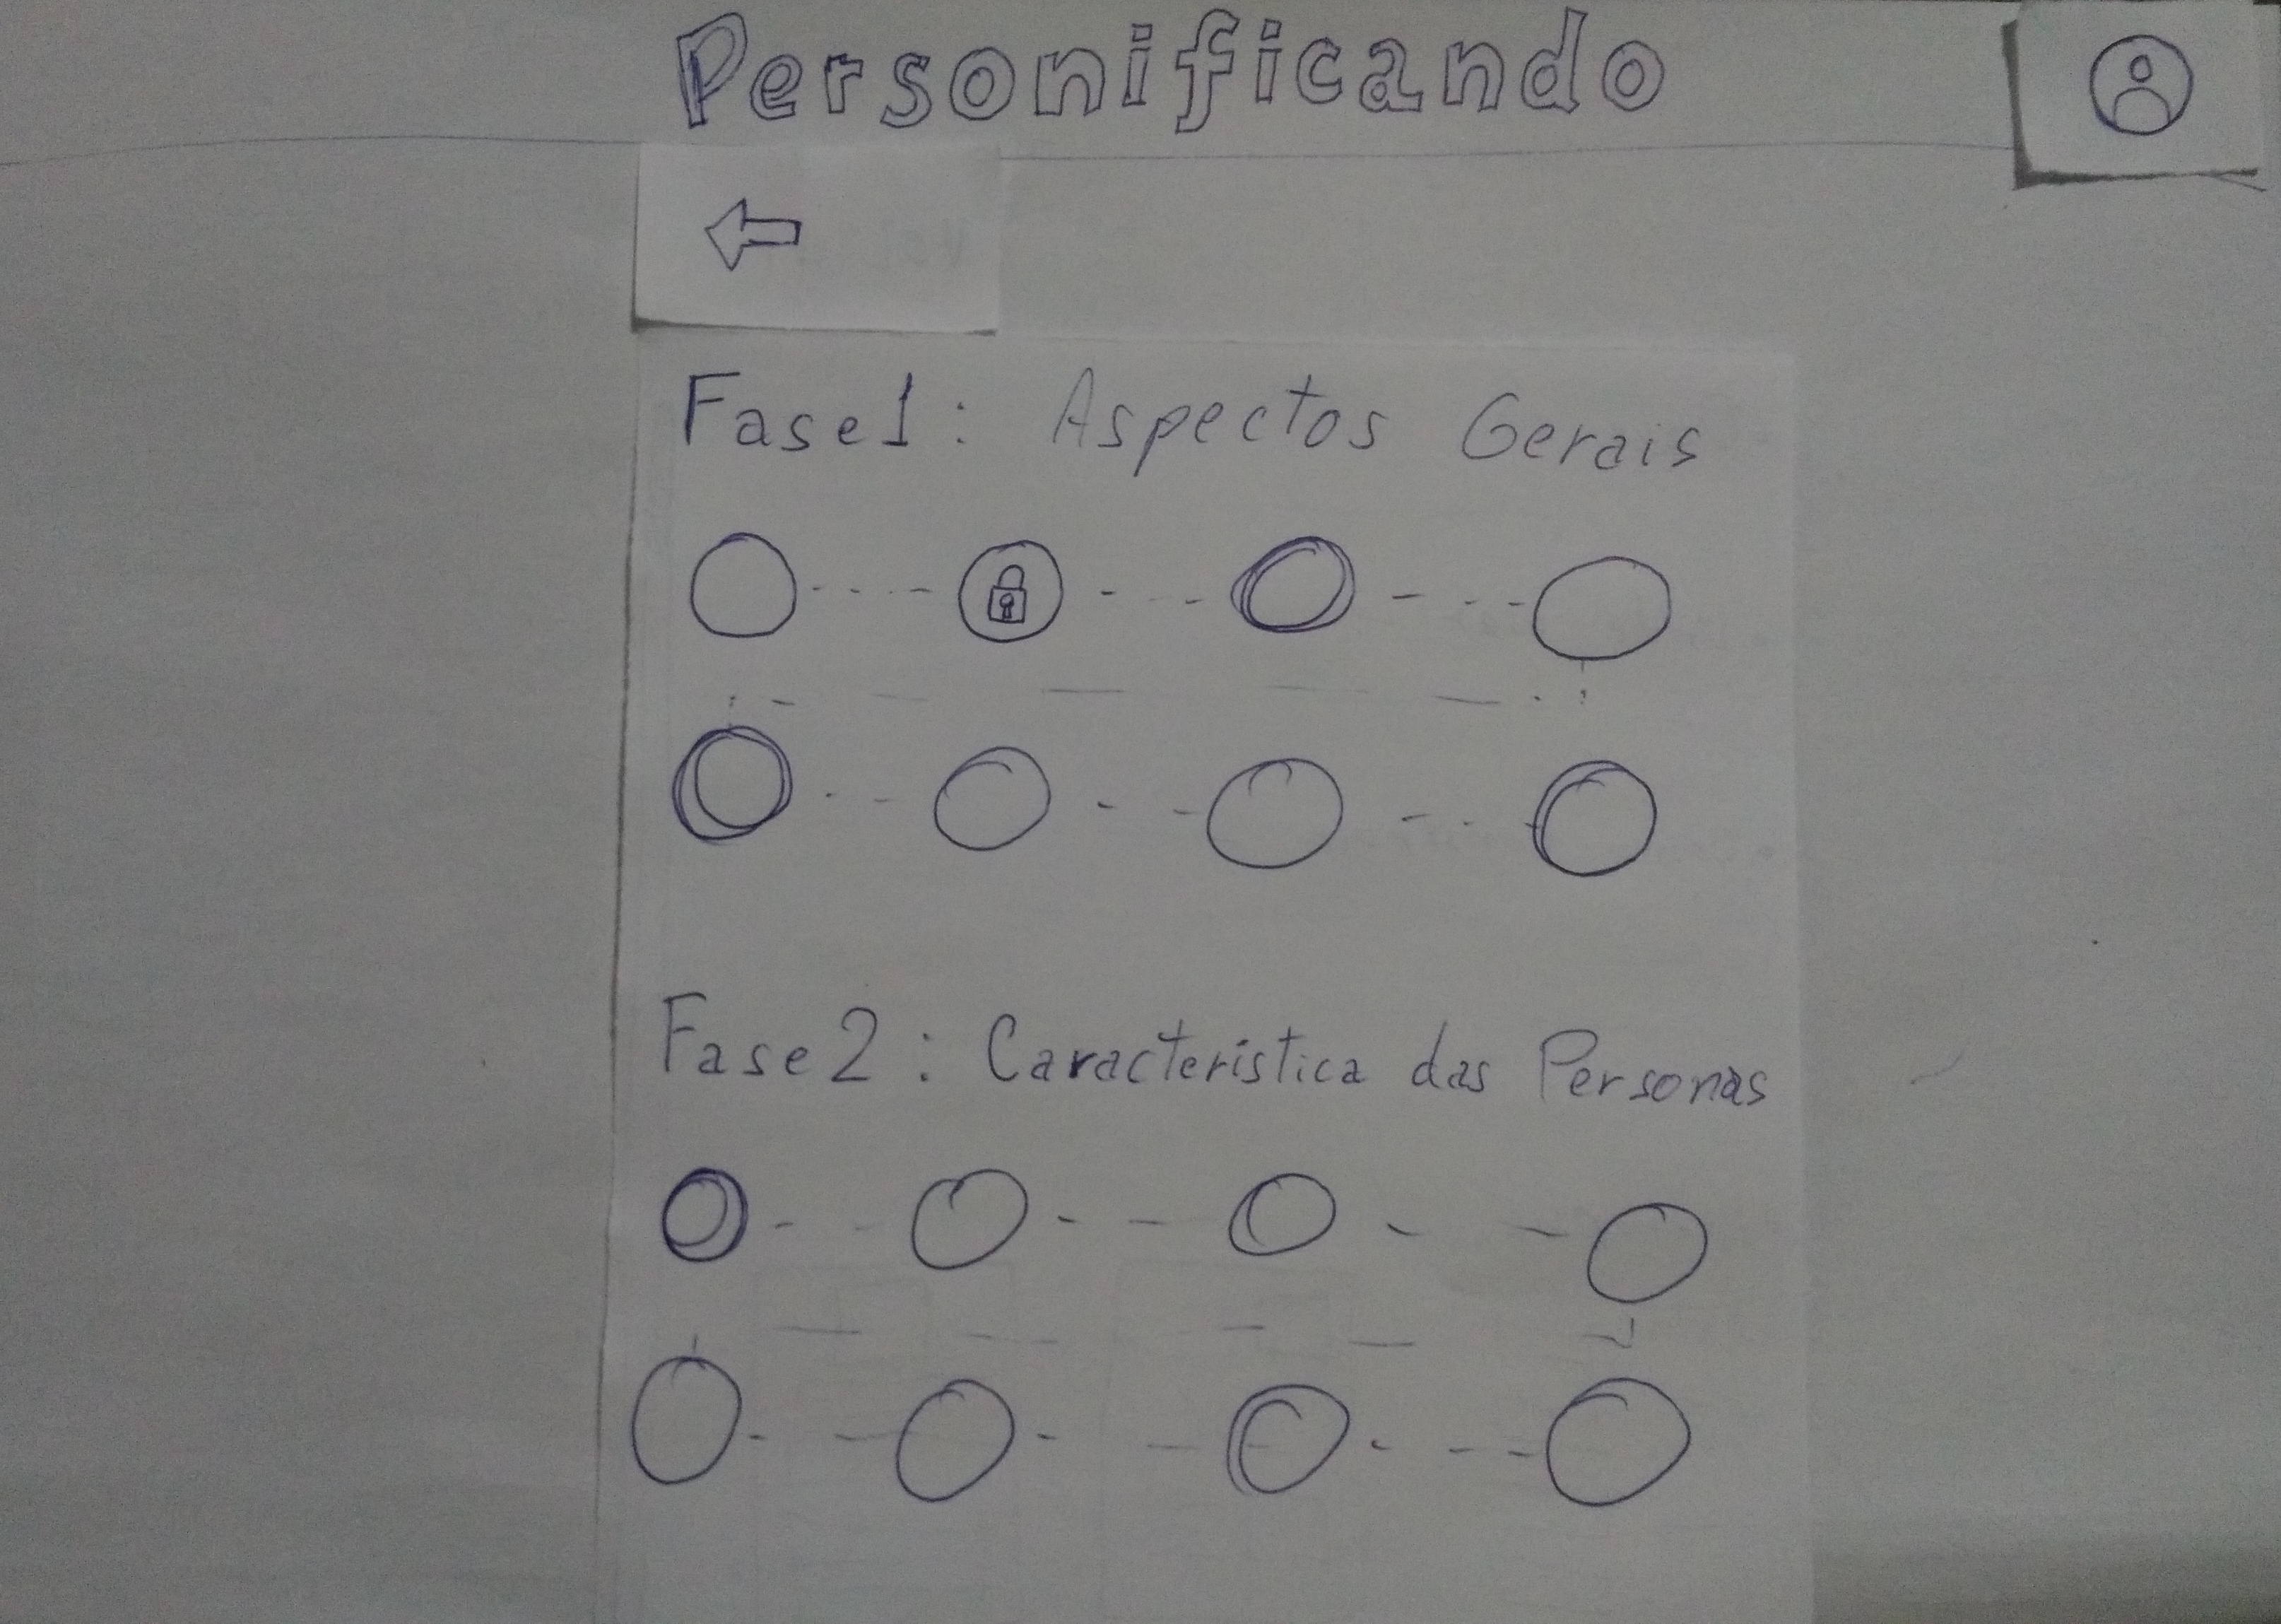
\includegraphics[keepaspectratio=true,scale=0.055]{figuras/prototype/proto6.jpg}
        \label{Fig:menu_fases.png}
    }
	\caption{Telas do Protótipo de Papel 1 - Próprio Autor}
	\label{Fig:proto1.png}
\end{figure}

\begin{figure}[htbp]
	\centering
    \subfigure[Menu das Fases - Iniciar Etapa]{
        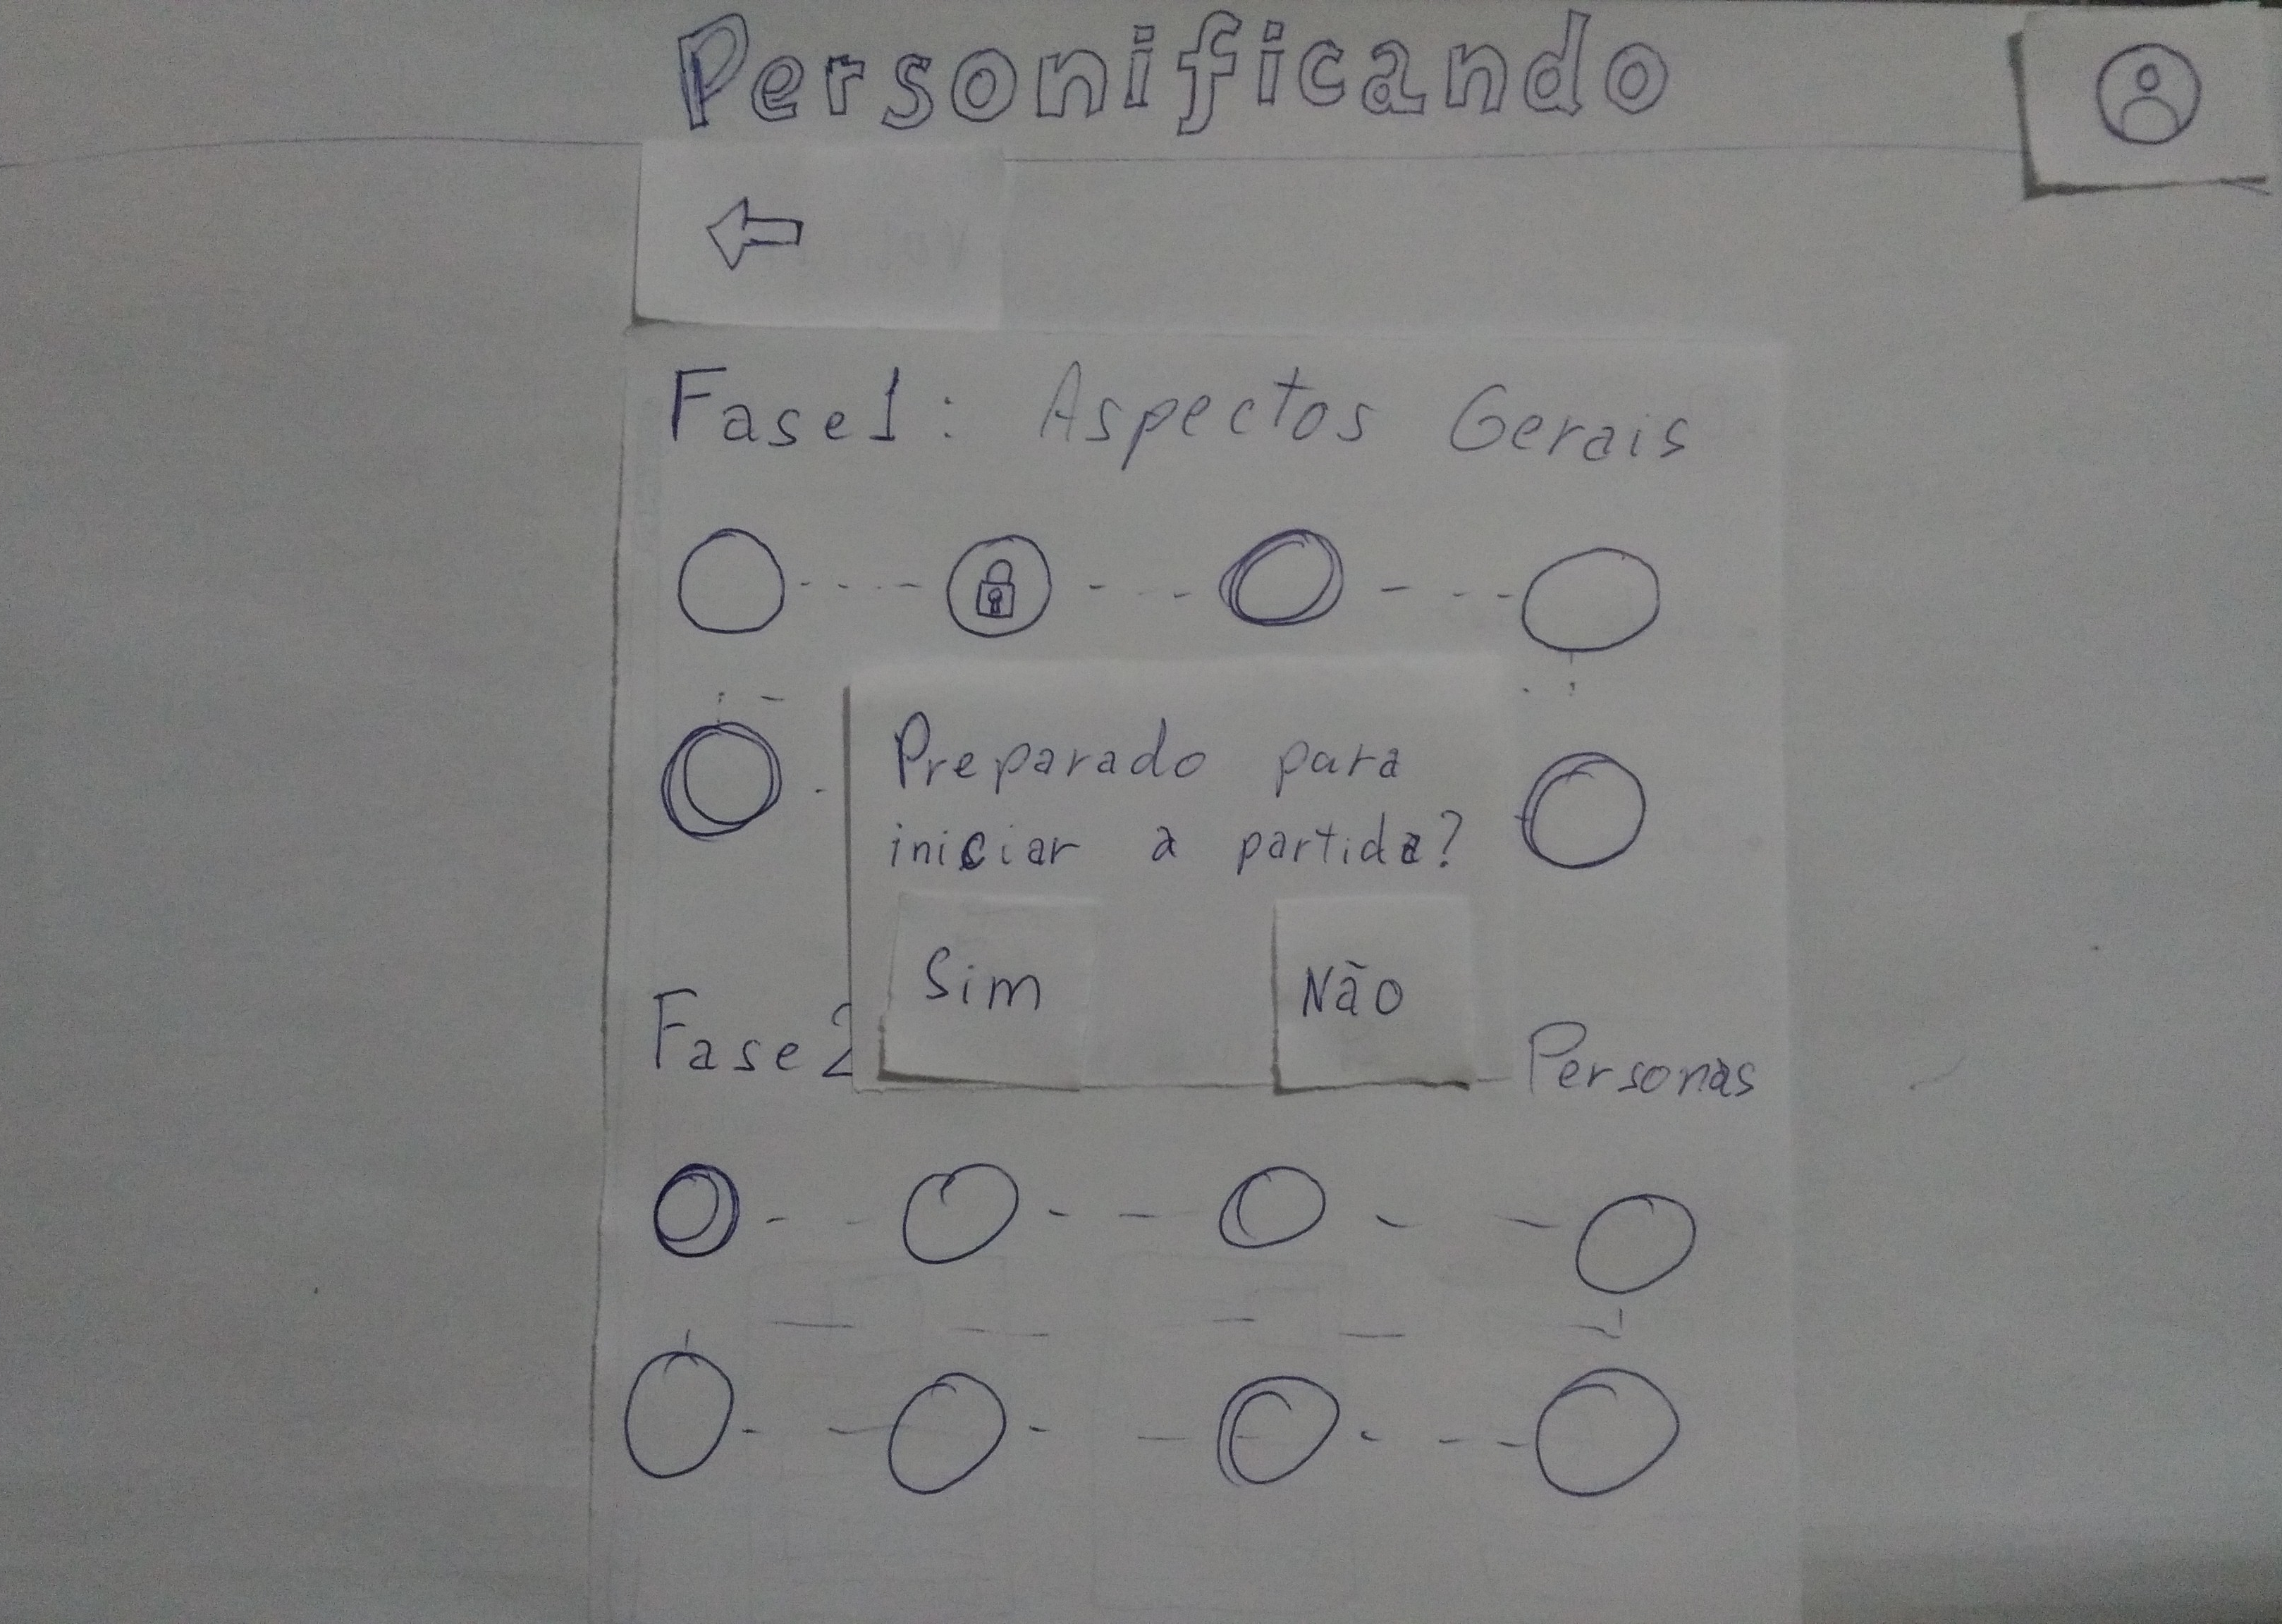
\includegraphics[keepaspectratio=true,scale=0.055]{figuras/prototype/proto7.jpg}
        \label{Fig:menu_etapa.png}
    }
    \quad
    \subfigure[Etapa - Conteúdo Inicial]{
        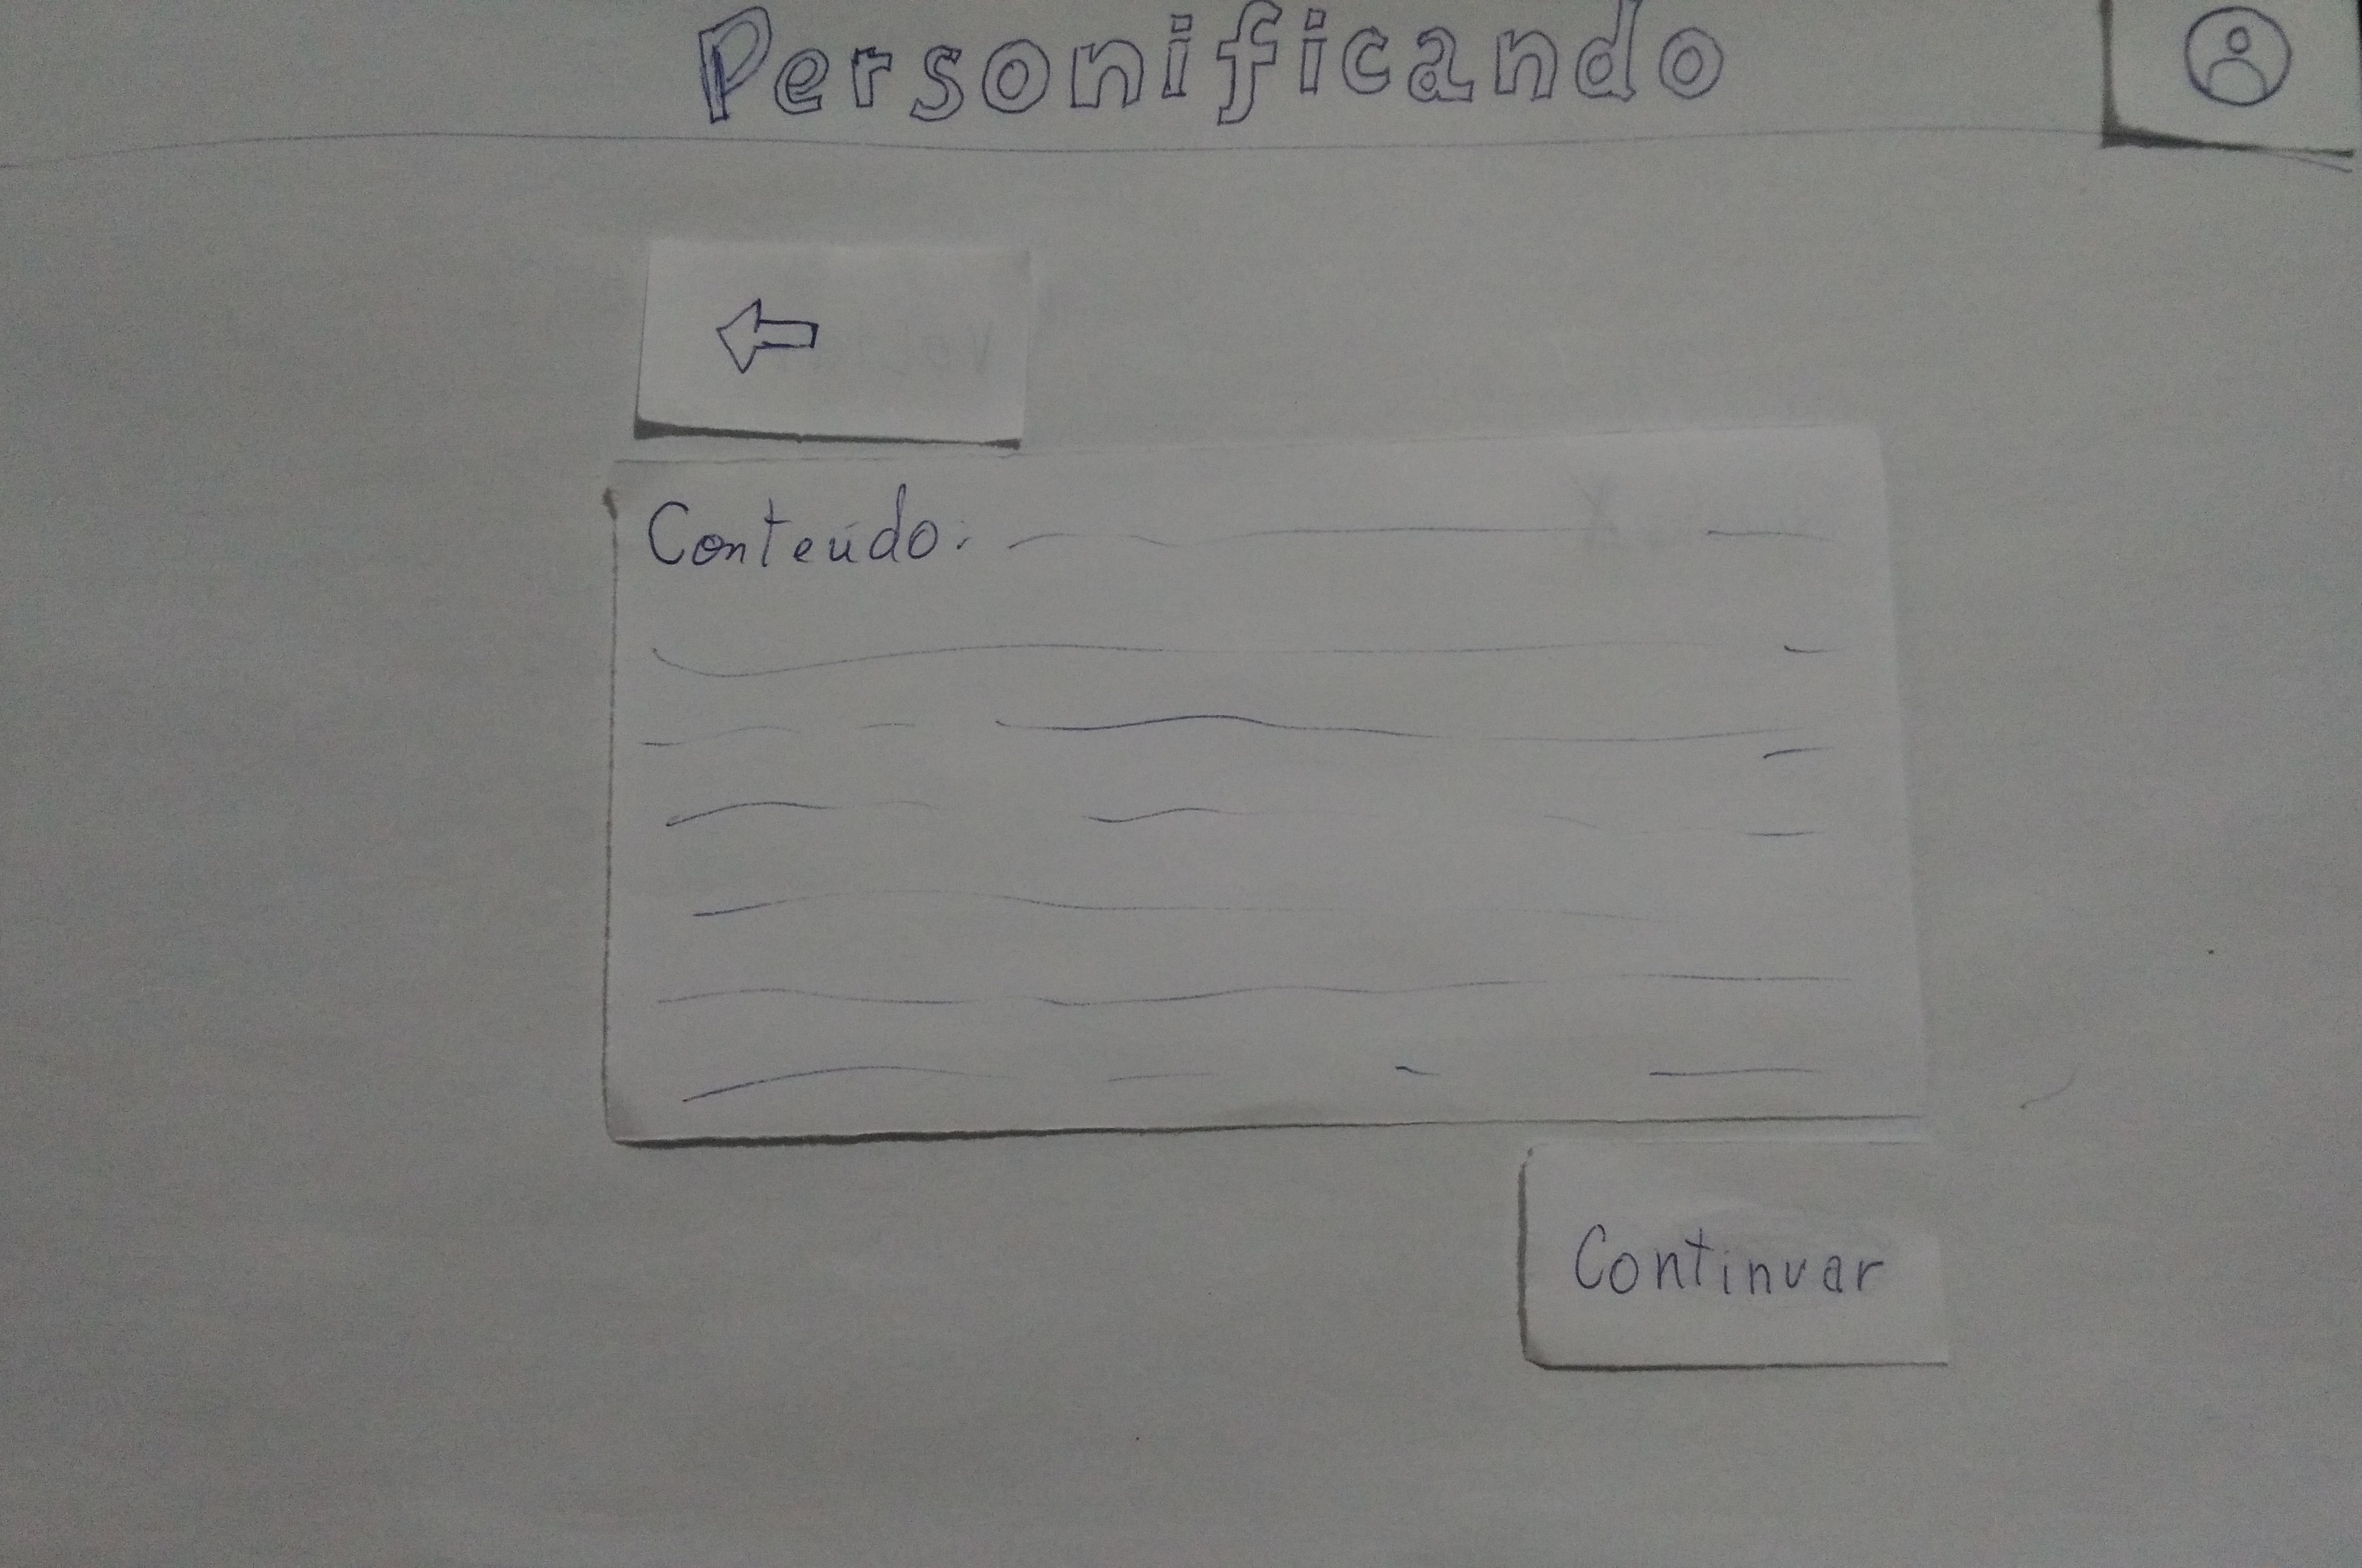
\includegraphics[keepaspectratio=true,scale=0.055]{figuras/prototype/proto8.jpg}
        \label{Fig:etapa_cont.png}
    }
    \quad
    \subfigure[Questão Múltipla Escolha]{  
	    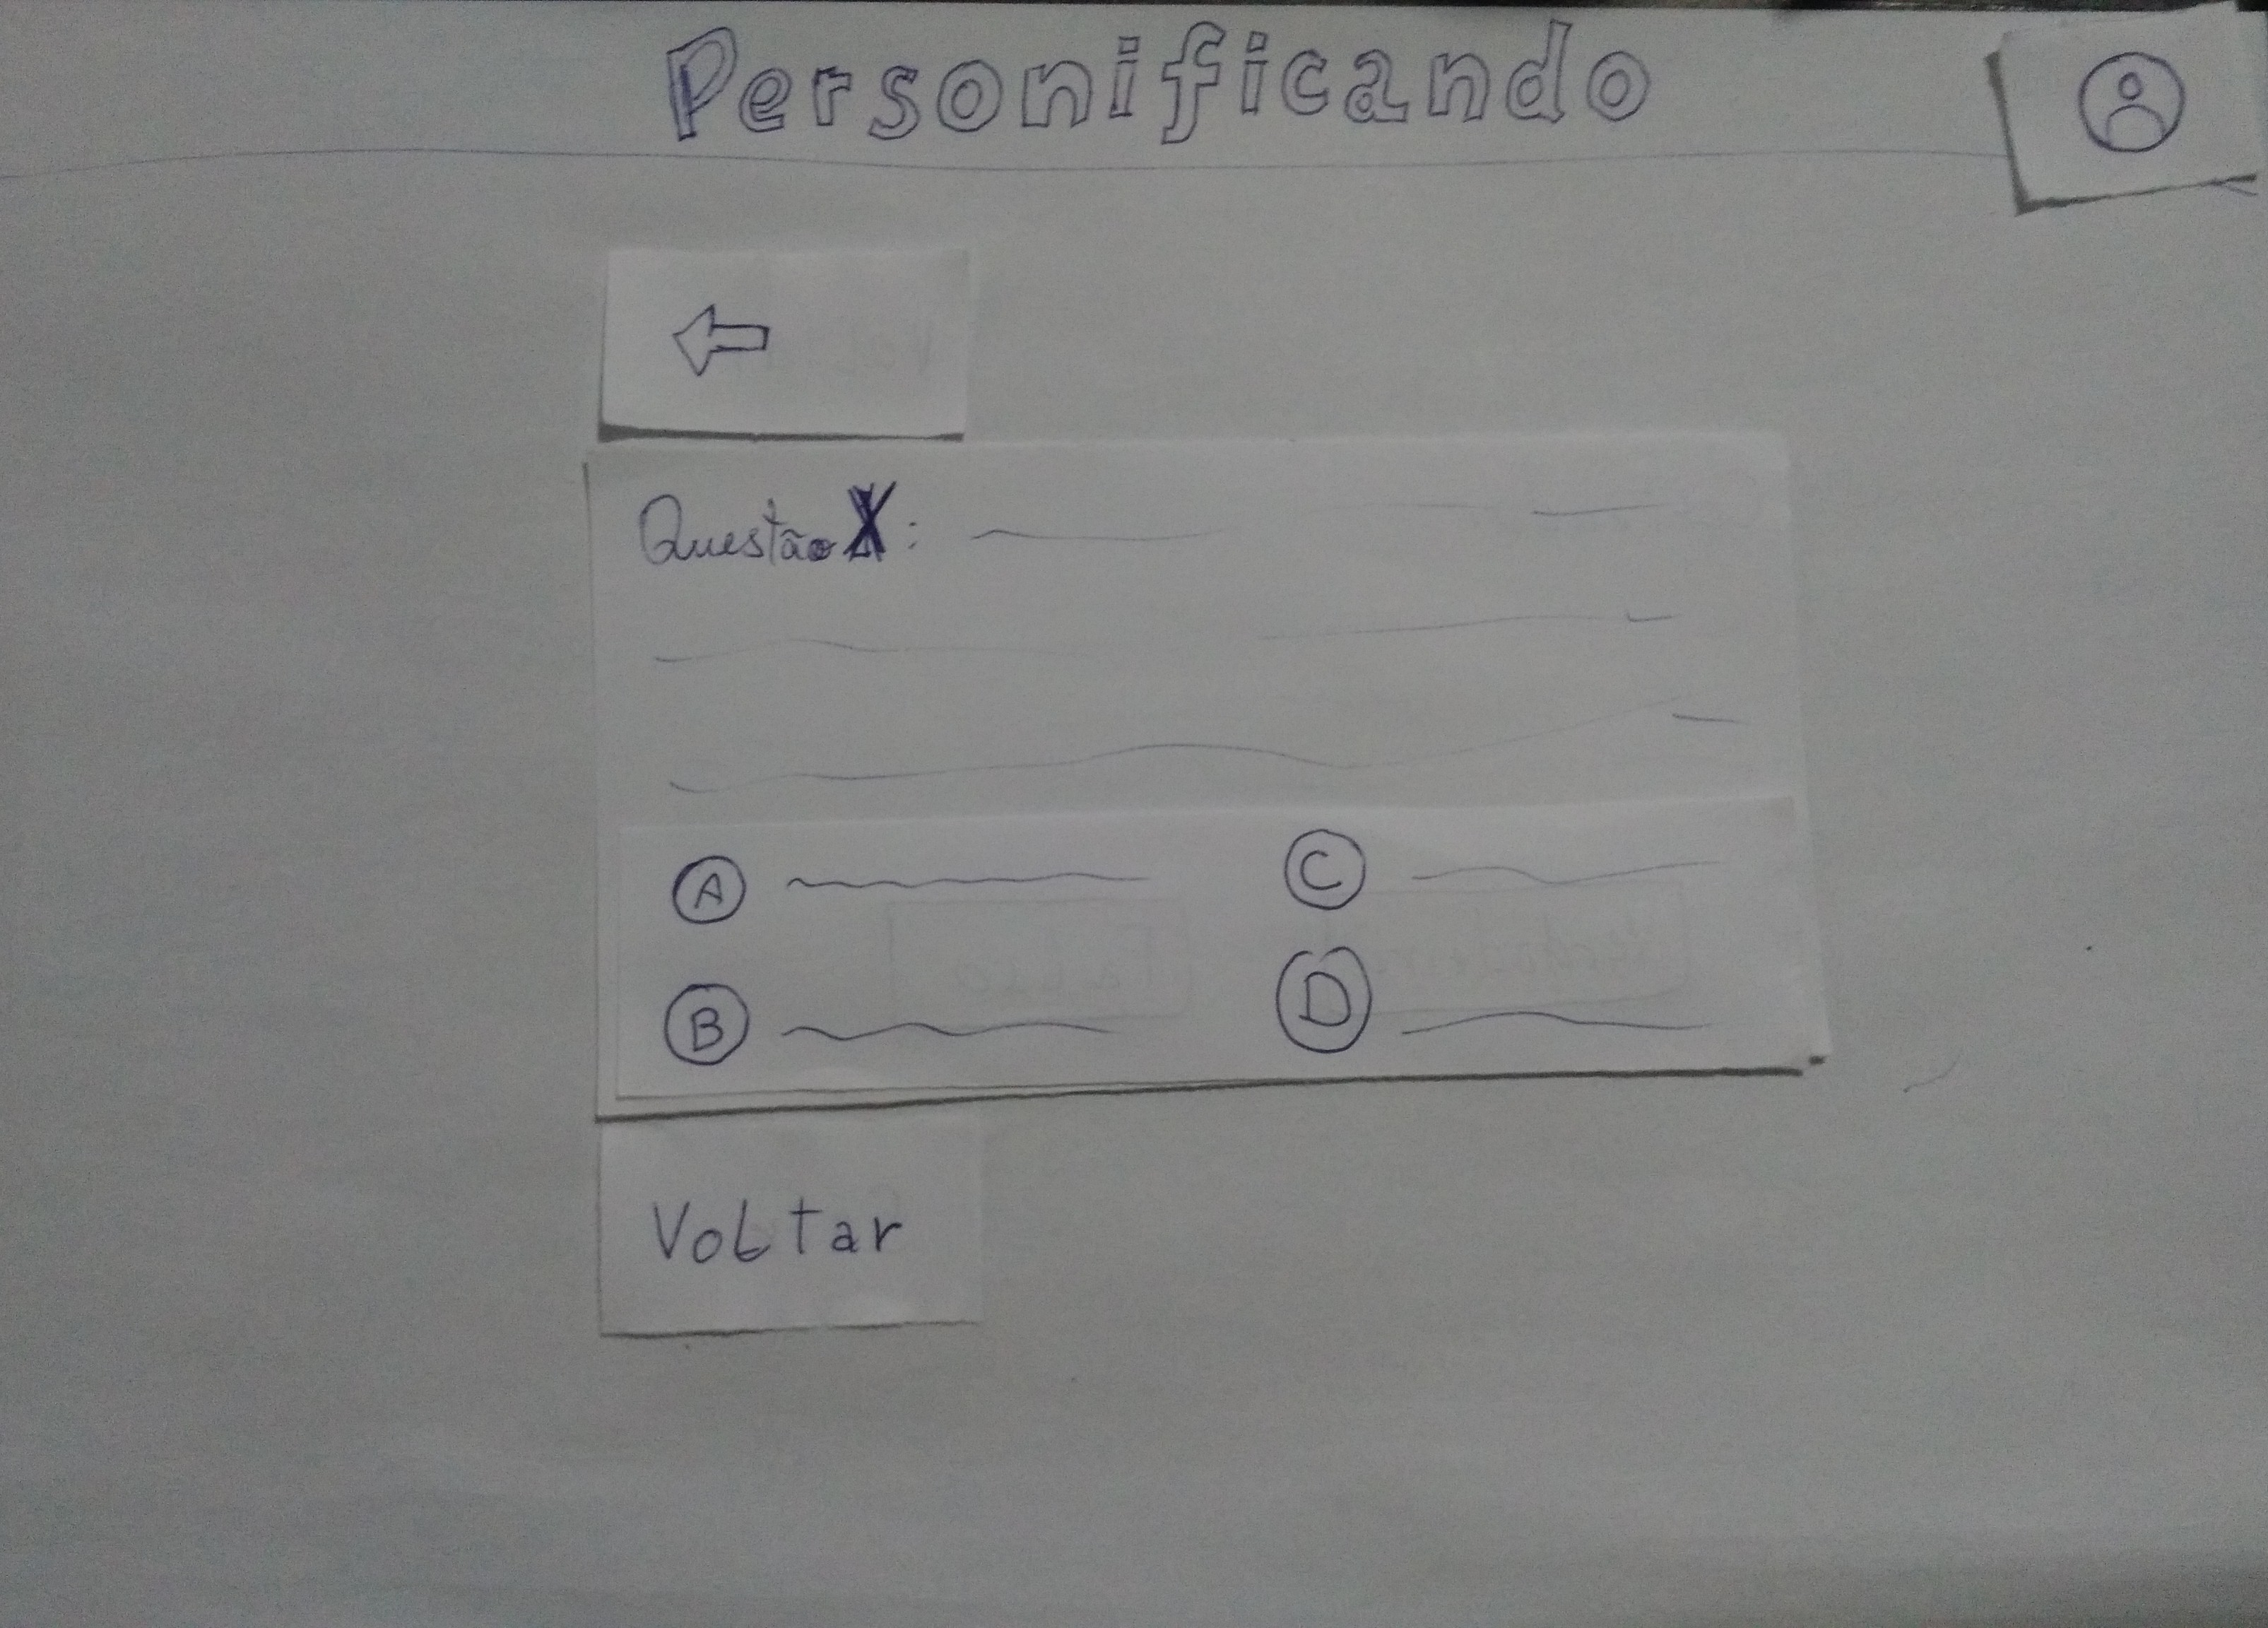
\includegraphics[keepaspectratio=true,scale=0.055]{figuras/prototype/proto9.jpg}
        \label{Fig:quest_mult.png}
    }
    \quad
    \subfigure[Questão Verdadeiro ou Falso]{
        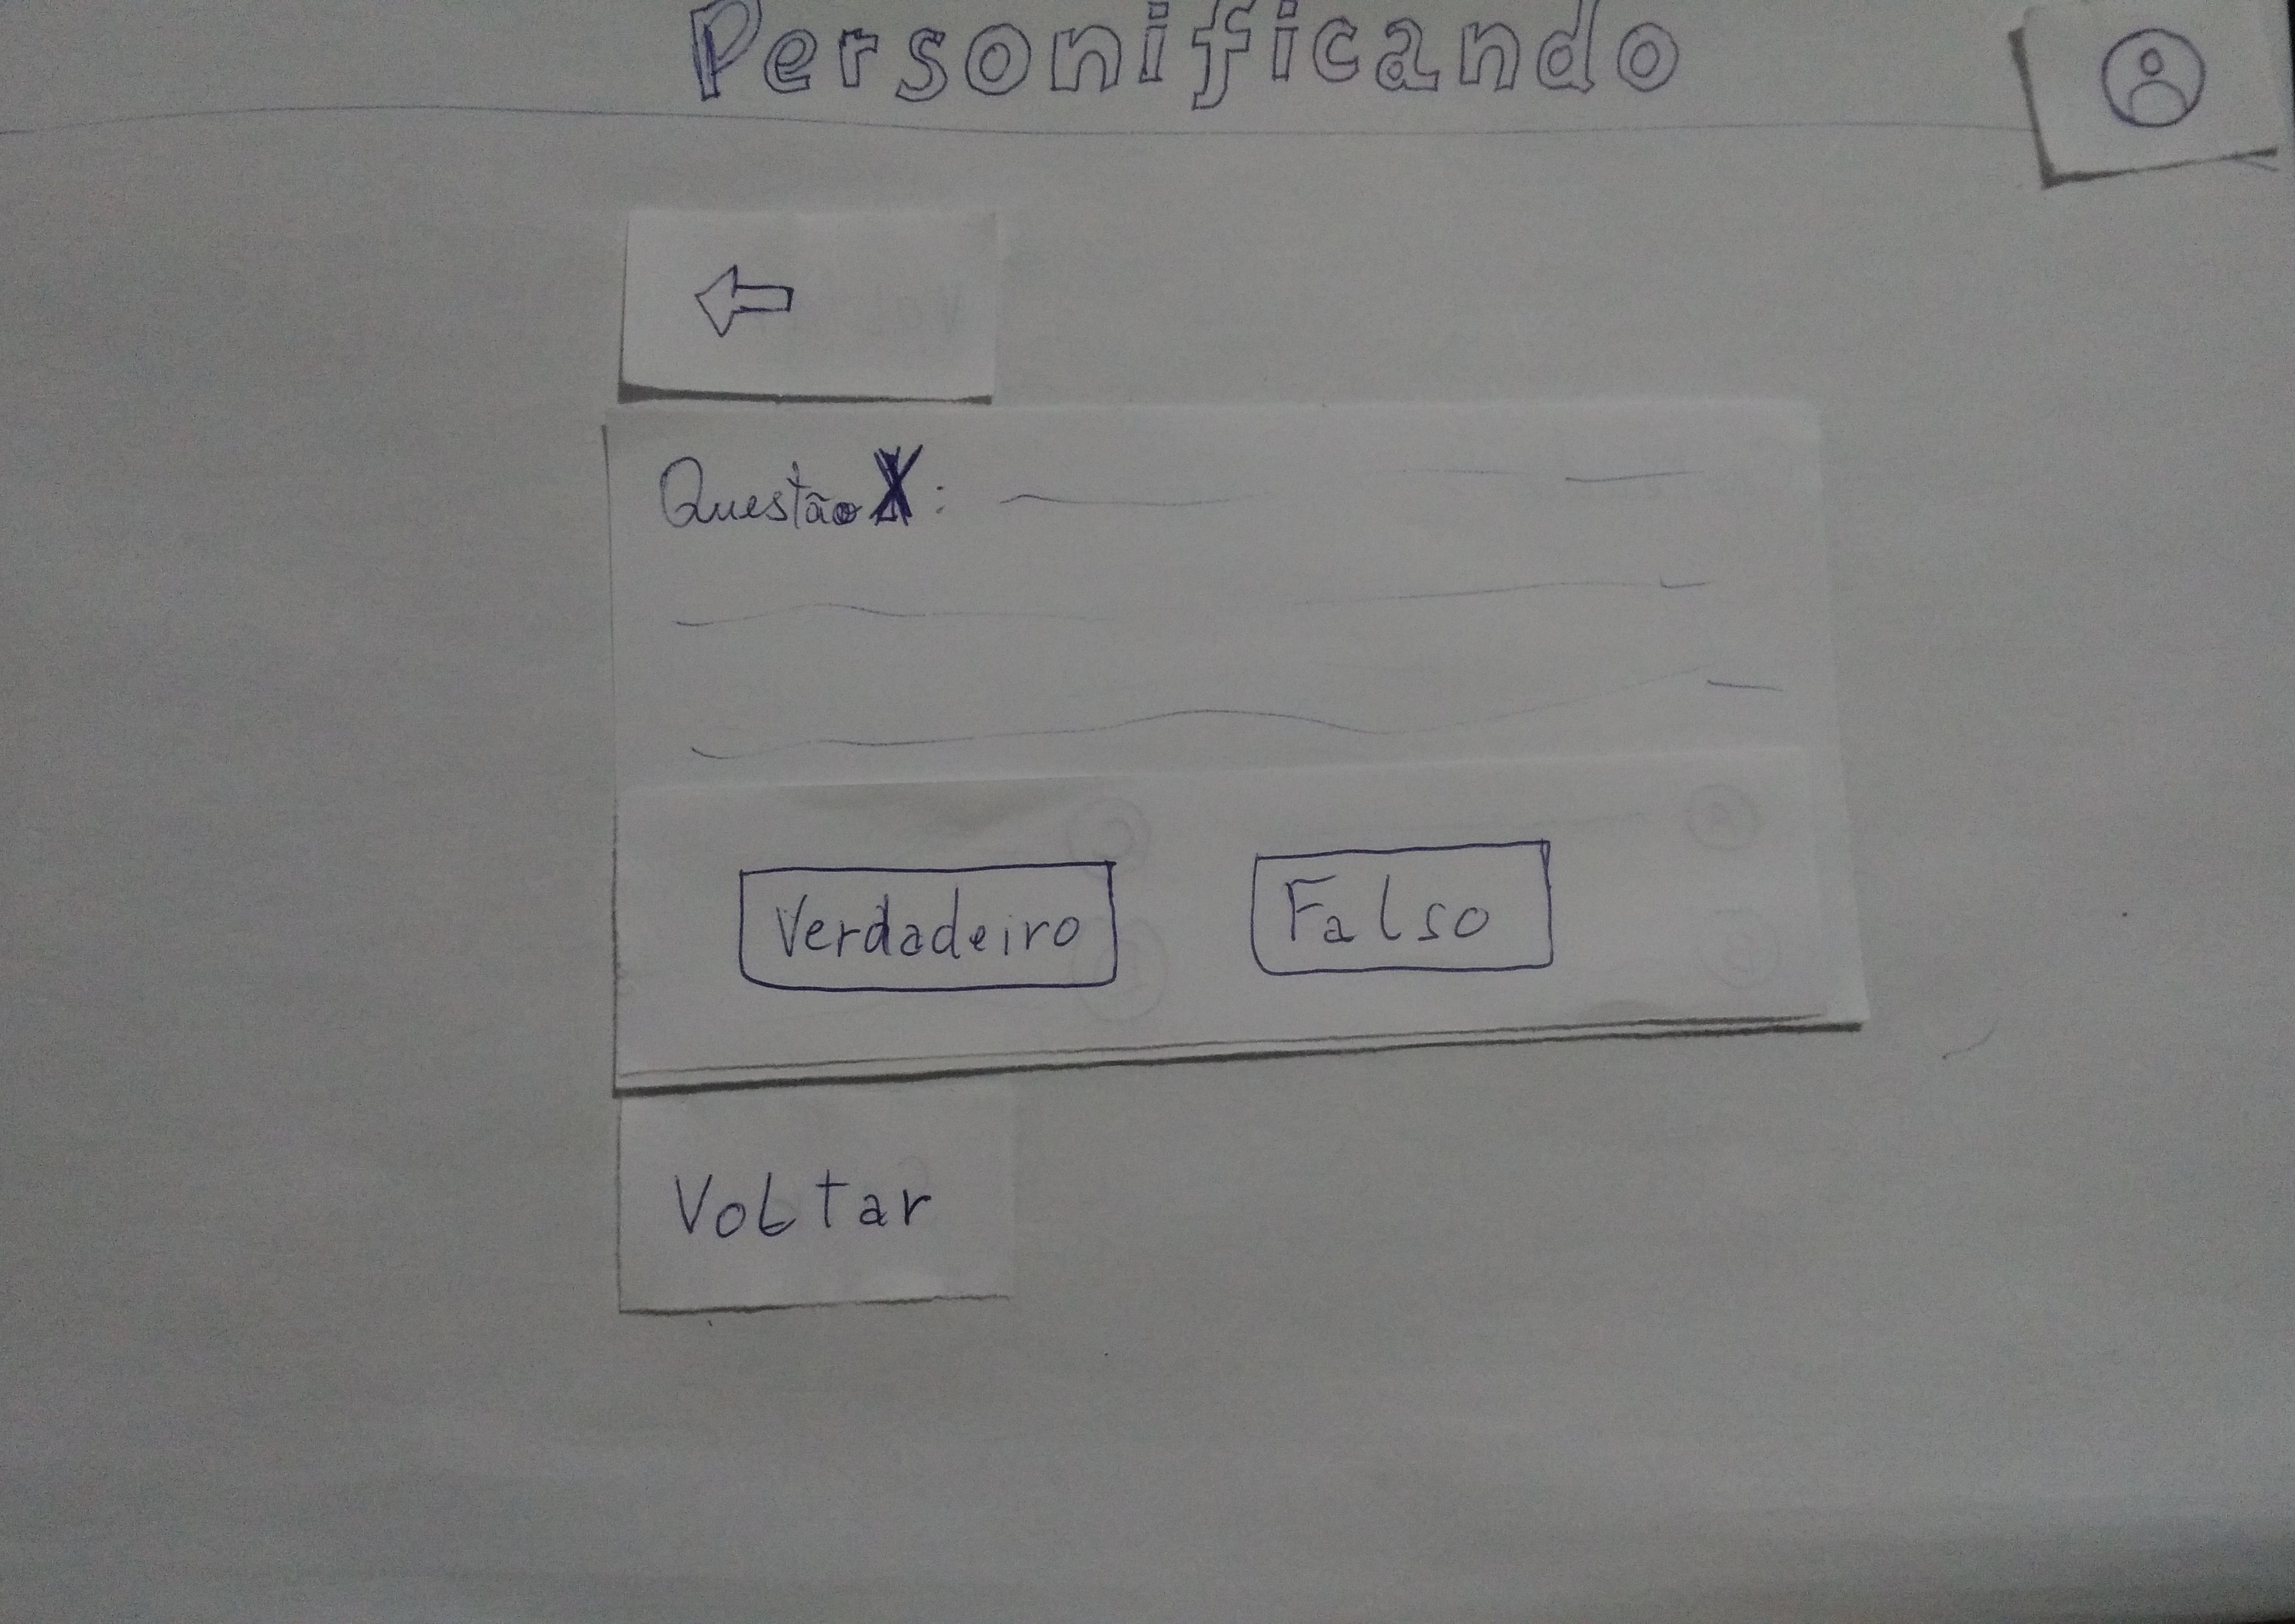
\includegraphics[keepaspectratio=true,scale=0.055]{figuras/prototype/proto10.jpg}
        \label{Fig:quest_vef.png}
    }
    \quad
    \subfigure[Questão - Confirmar Resposta]{
        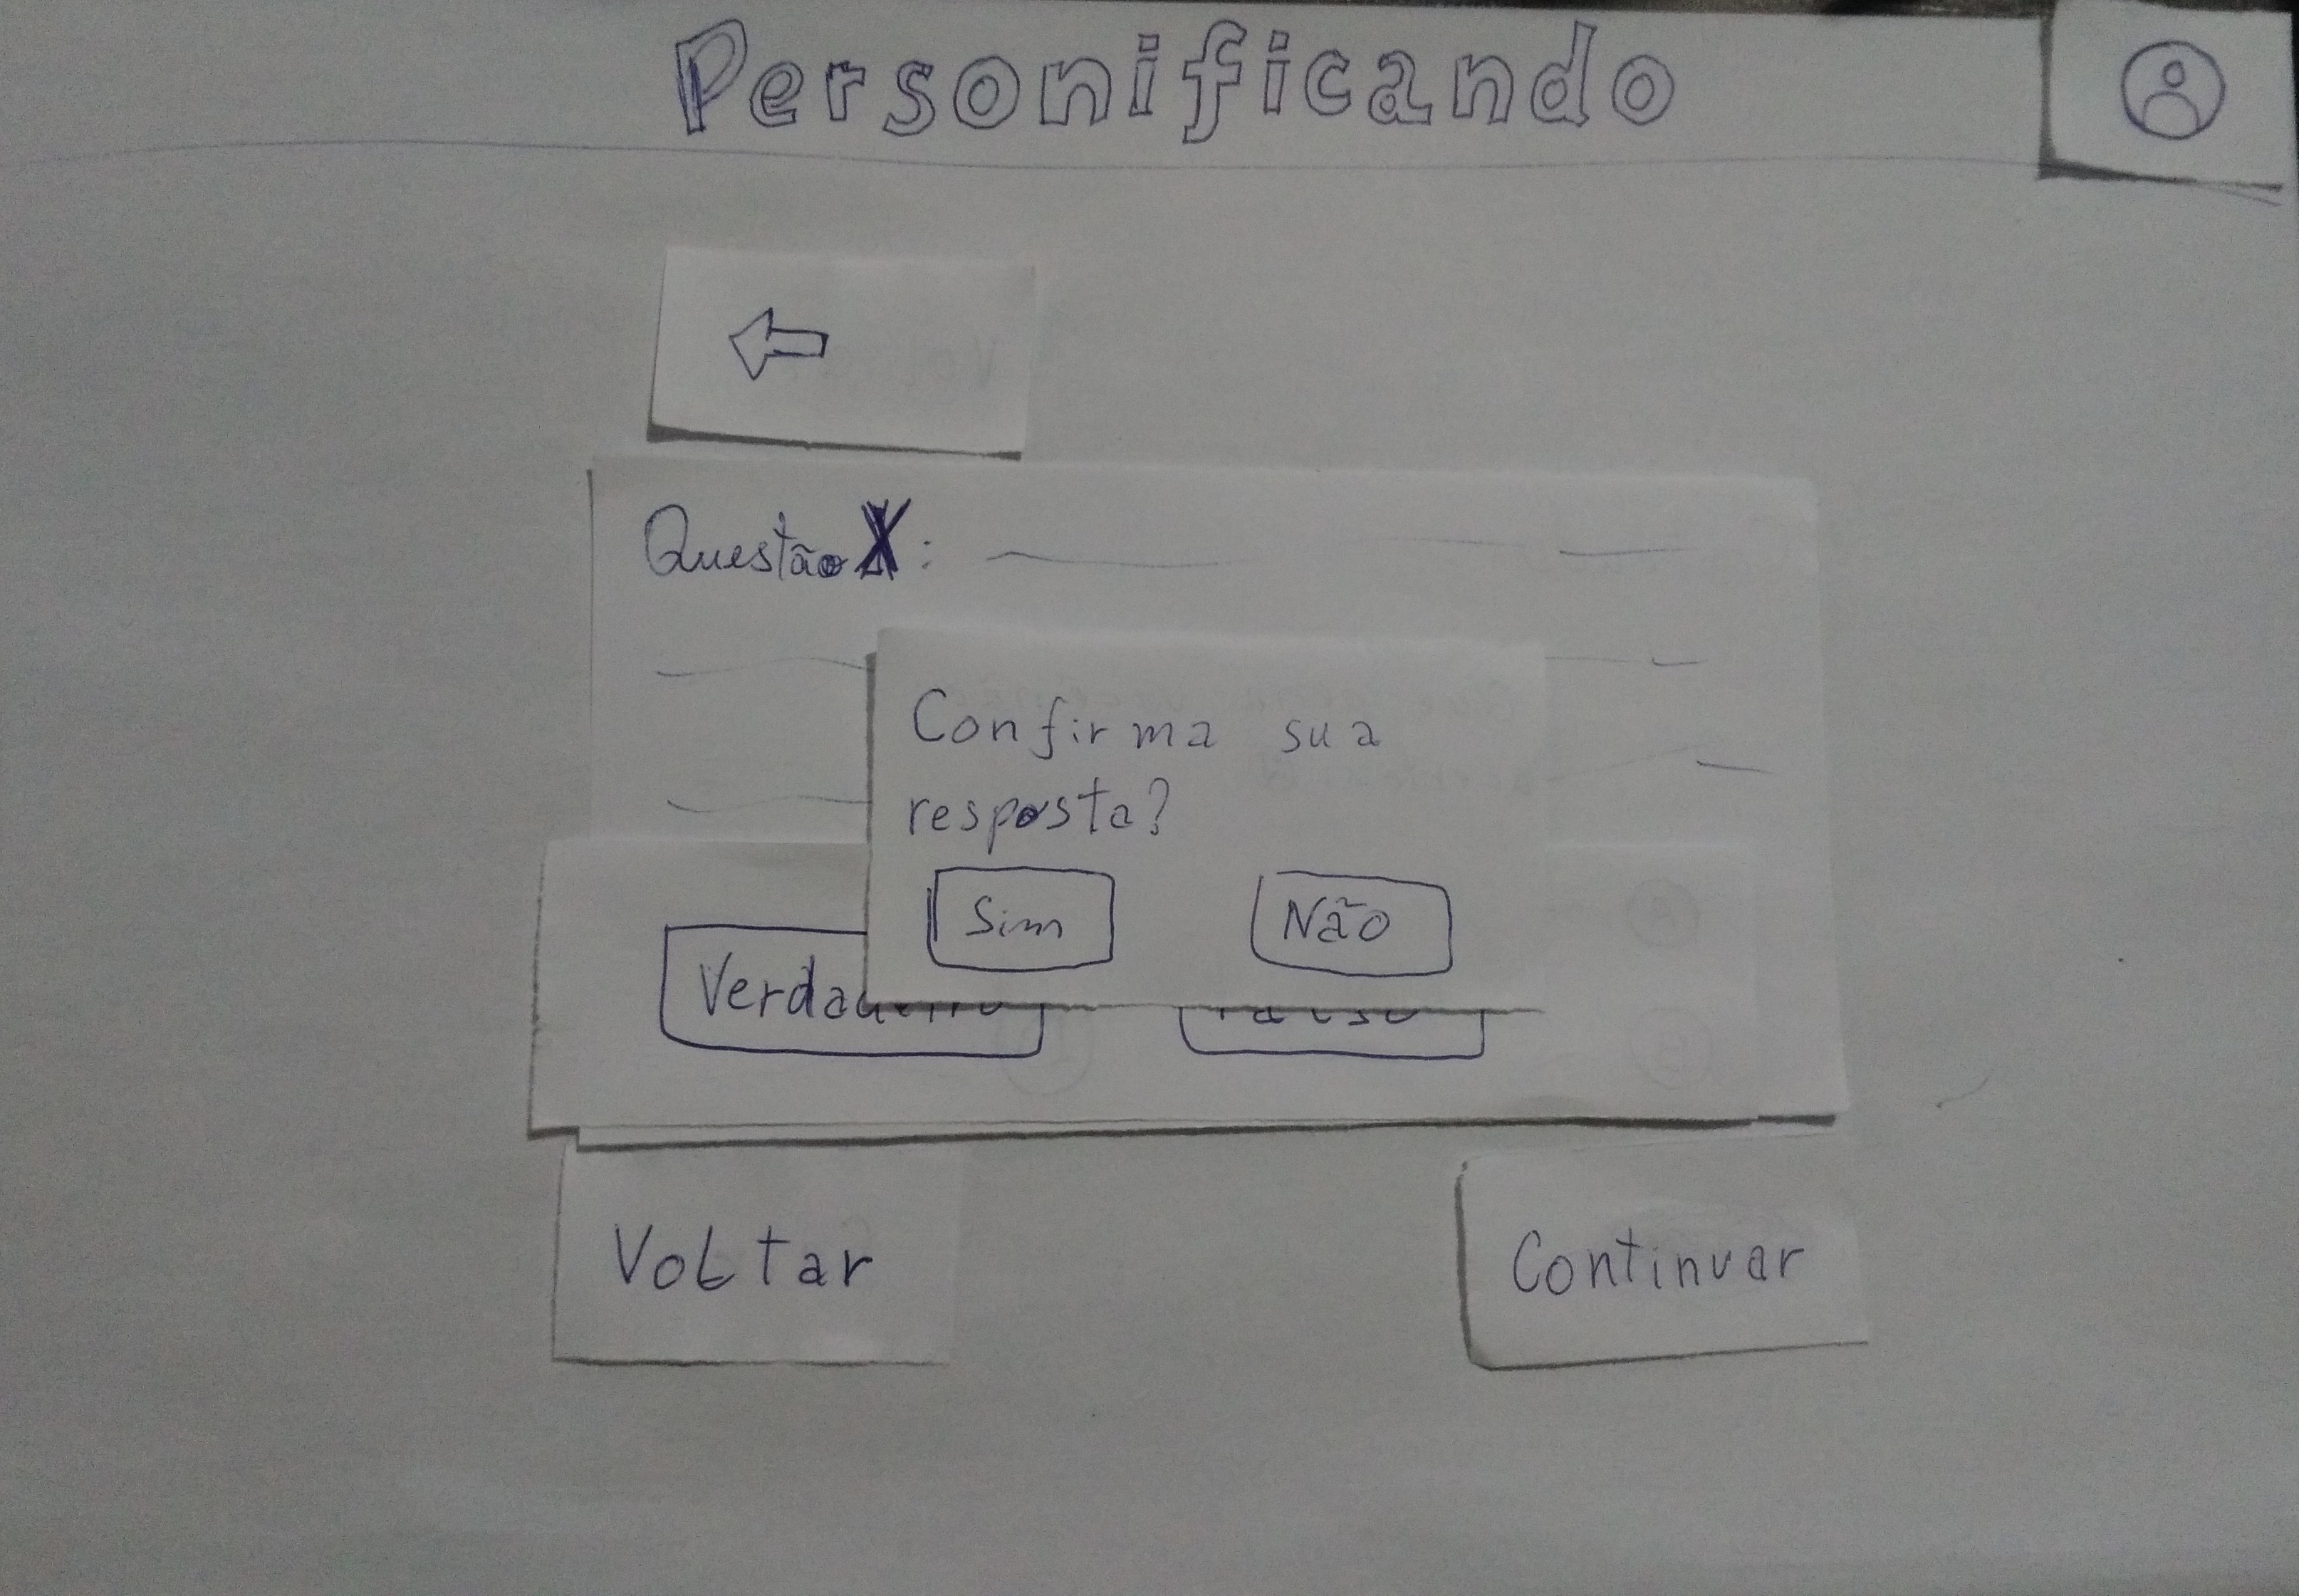
\includegraphics[keepaspectratio=true,scale=0.055]{figuras/prototype/proto11.jpg}
        \label{Fig:quest_confirm.png}
    }
    \quad
    \subfigure[Questão - Resposta Certa]{
        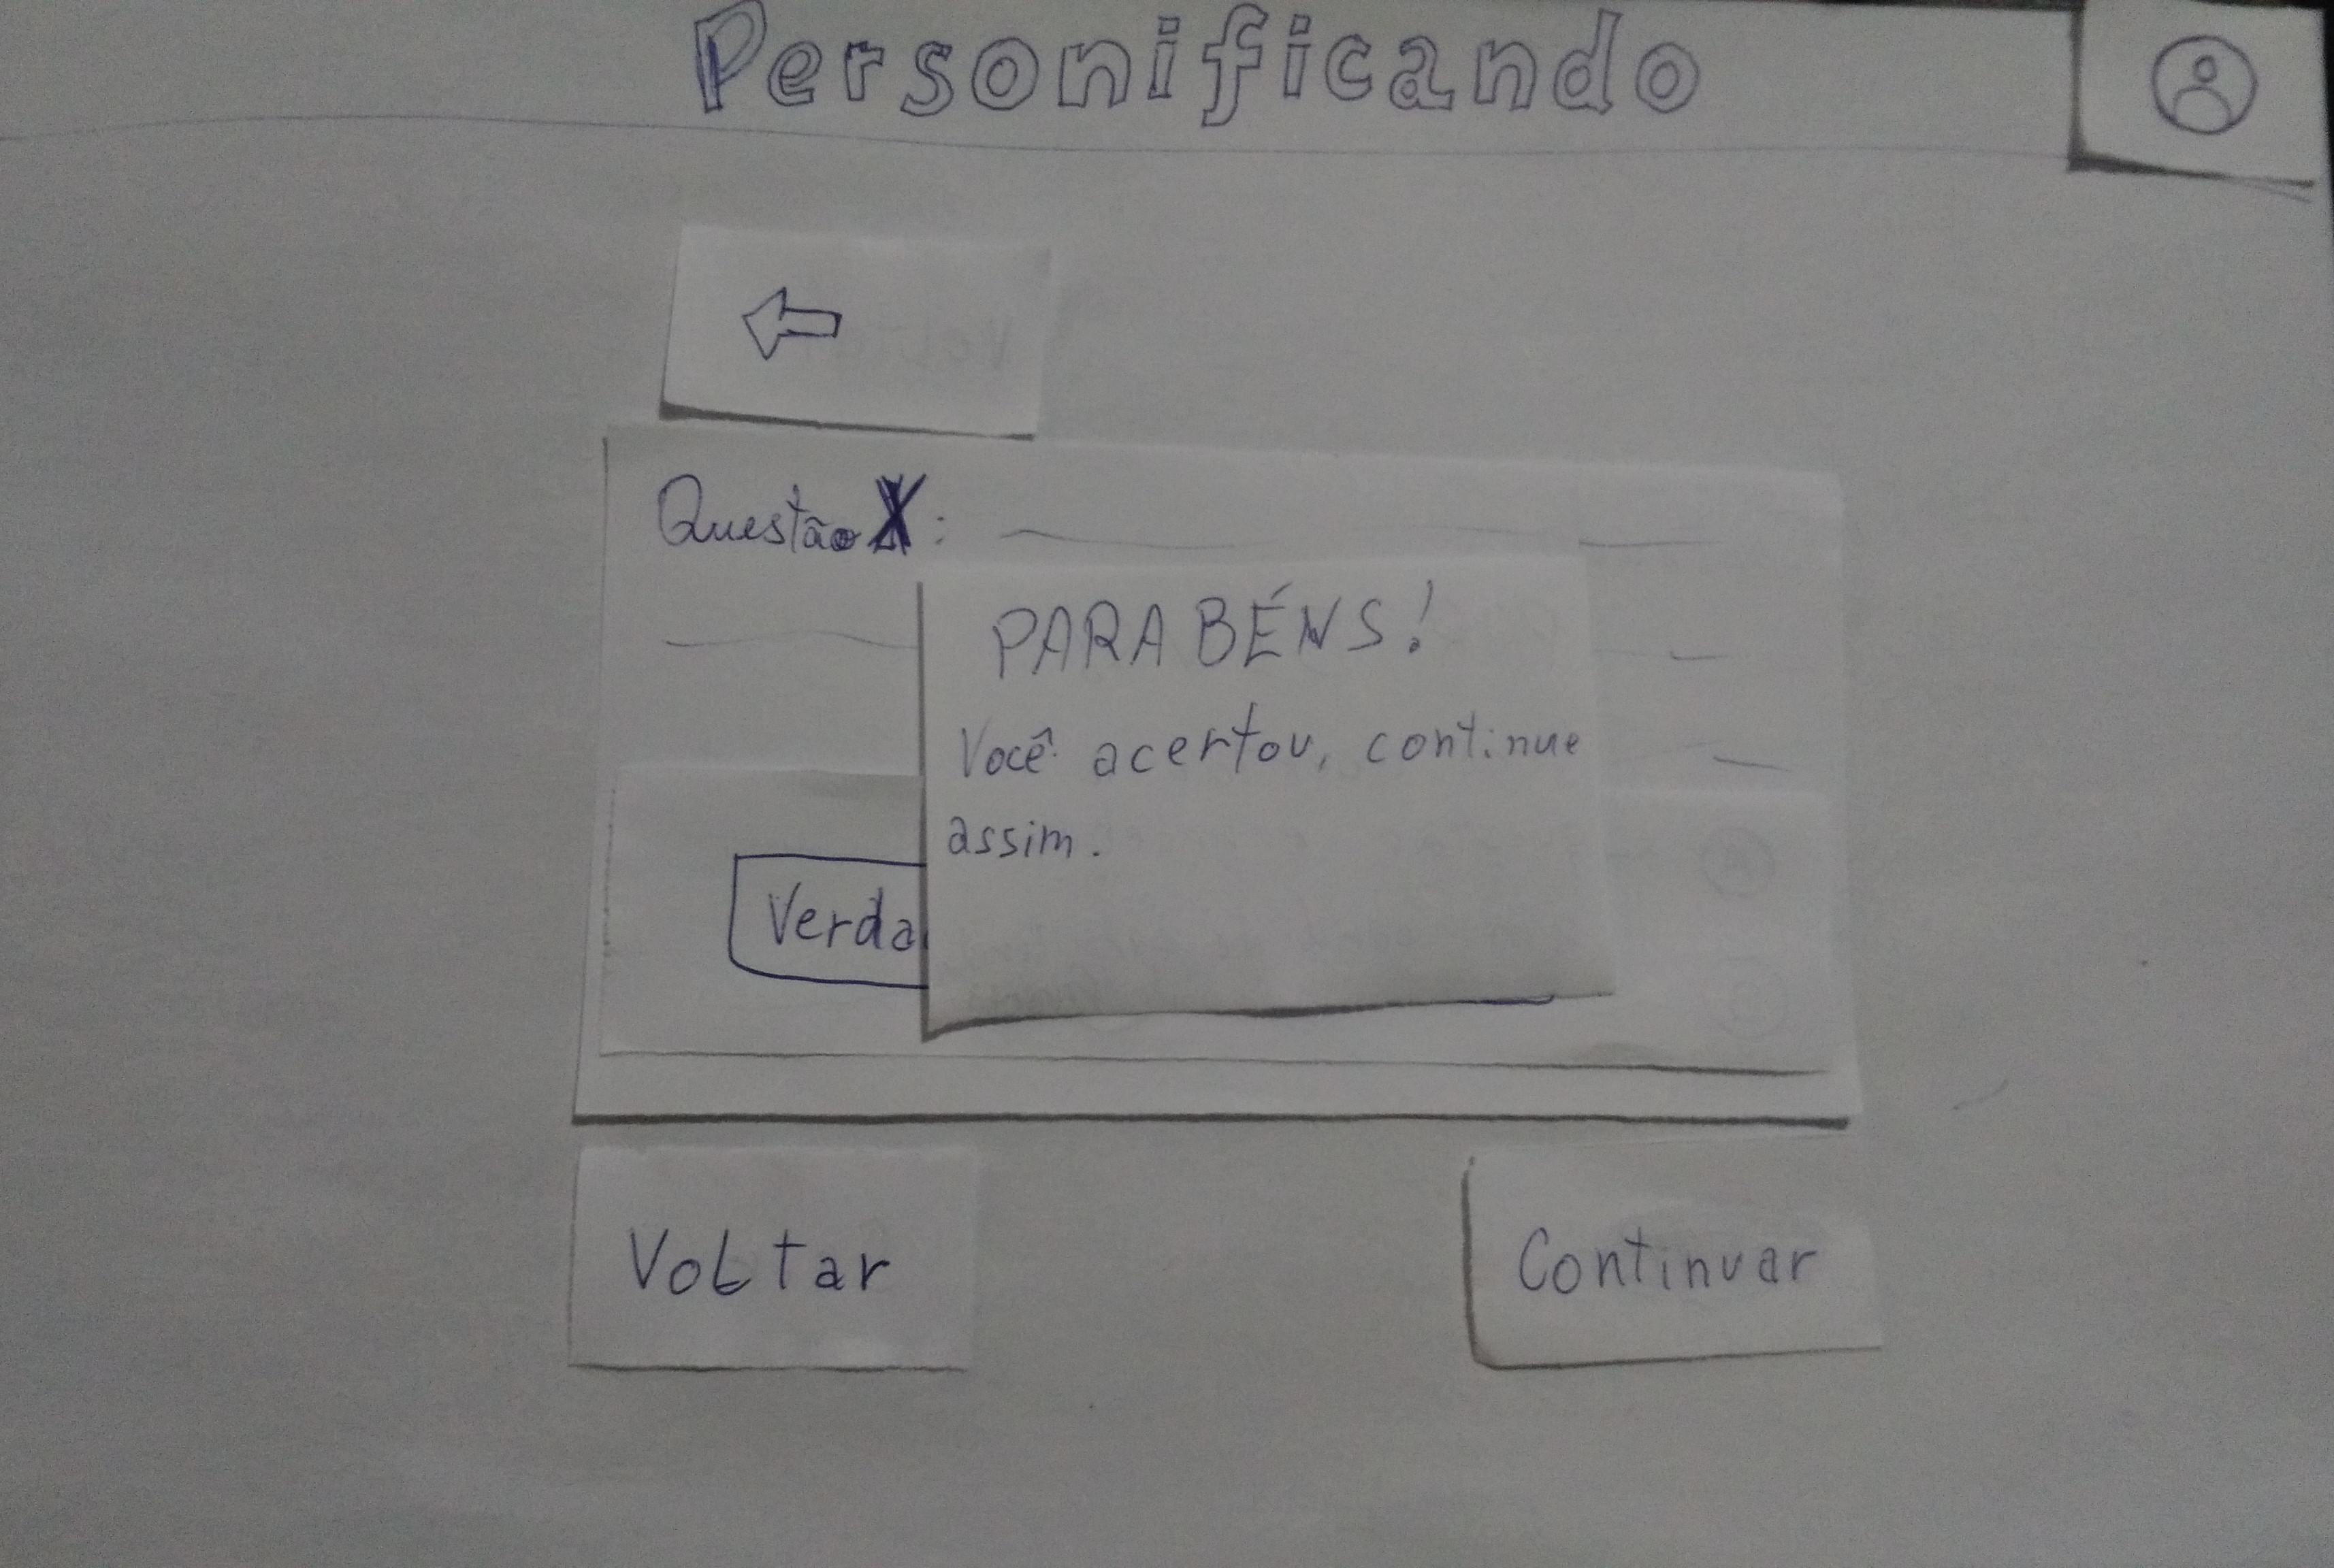
\includegraphics[keepaspectratio=true,scale=0.055]{figuras/prototype/proto12.jpg}
        \label{Fig:quest_certa.png}
    }
    
	\caption{Telas do Protótipo de Papel 2 - Próprio Autor}
	\label{Fig:proto2.png}
\end{figure}

\begin{figure}[htbp]
	\centering
	\subfigure[Questão - Resposta Certa e Recompensada]{
        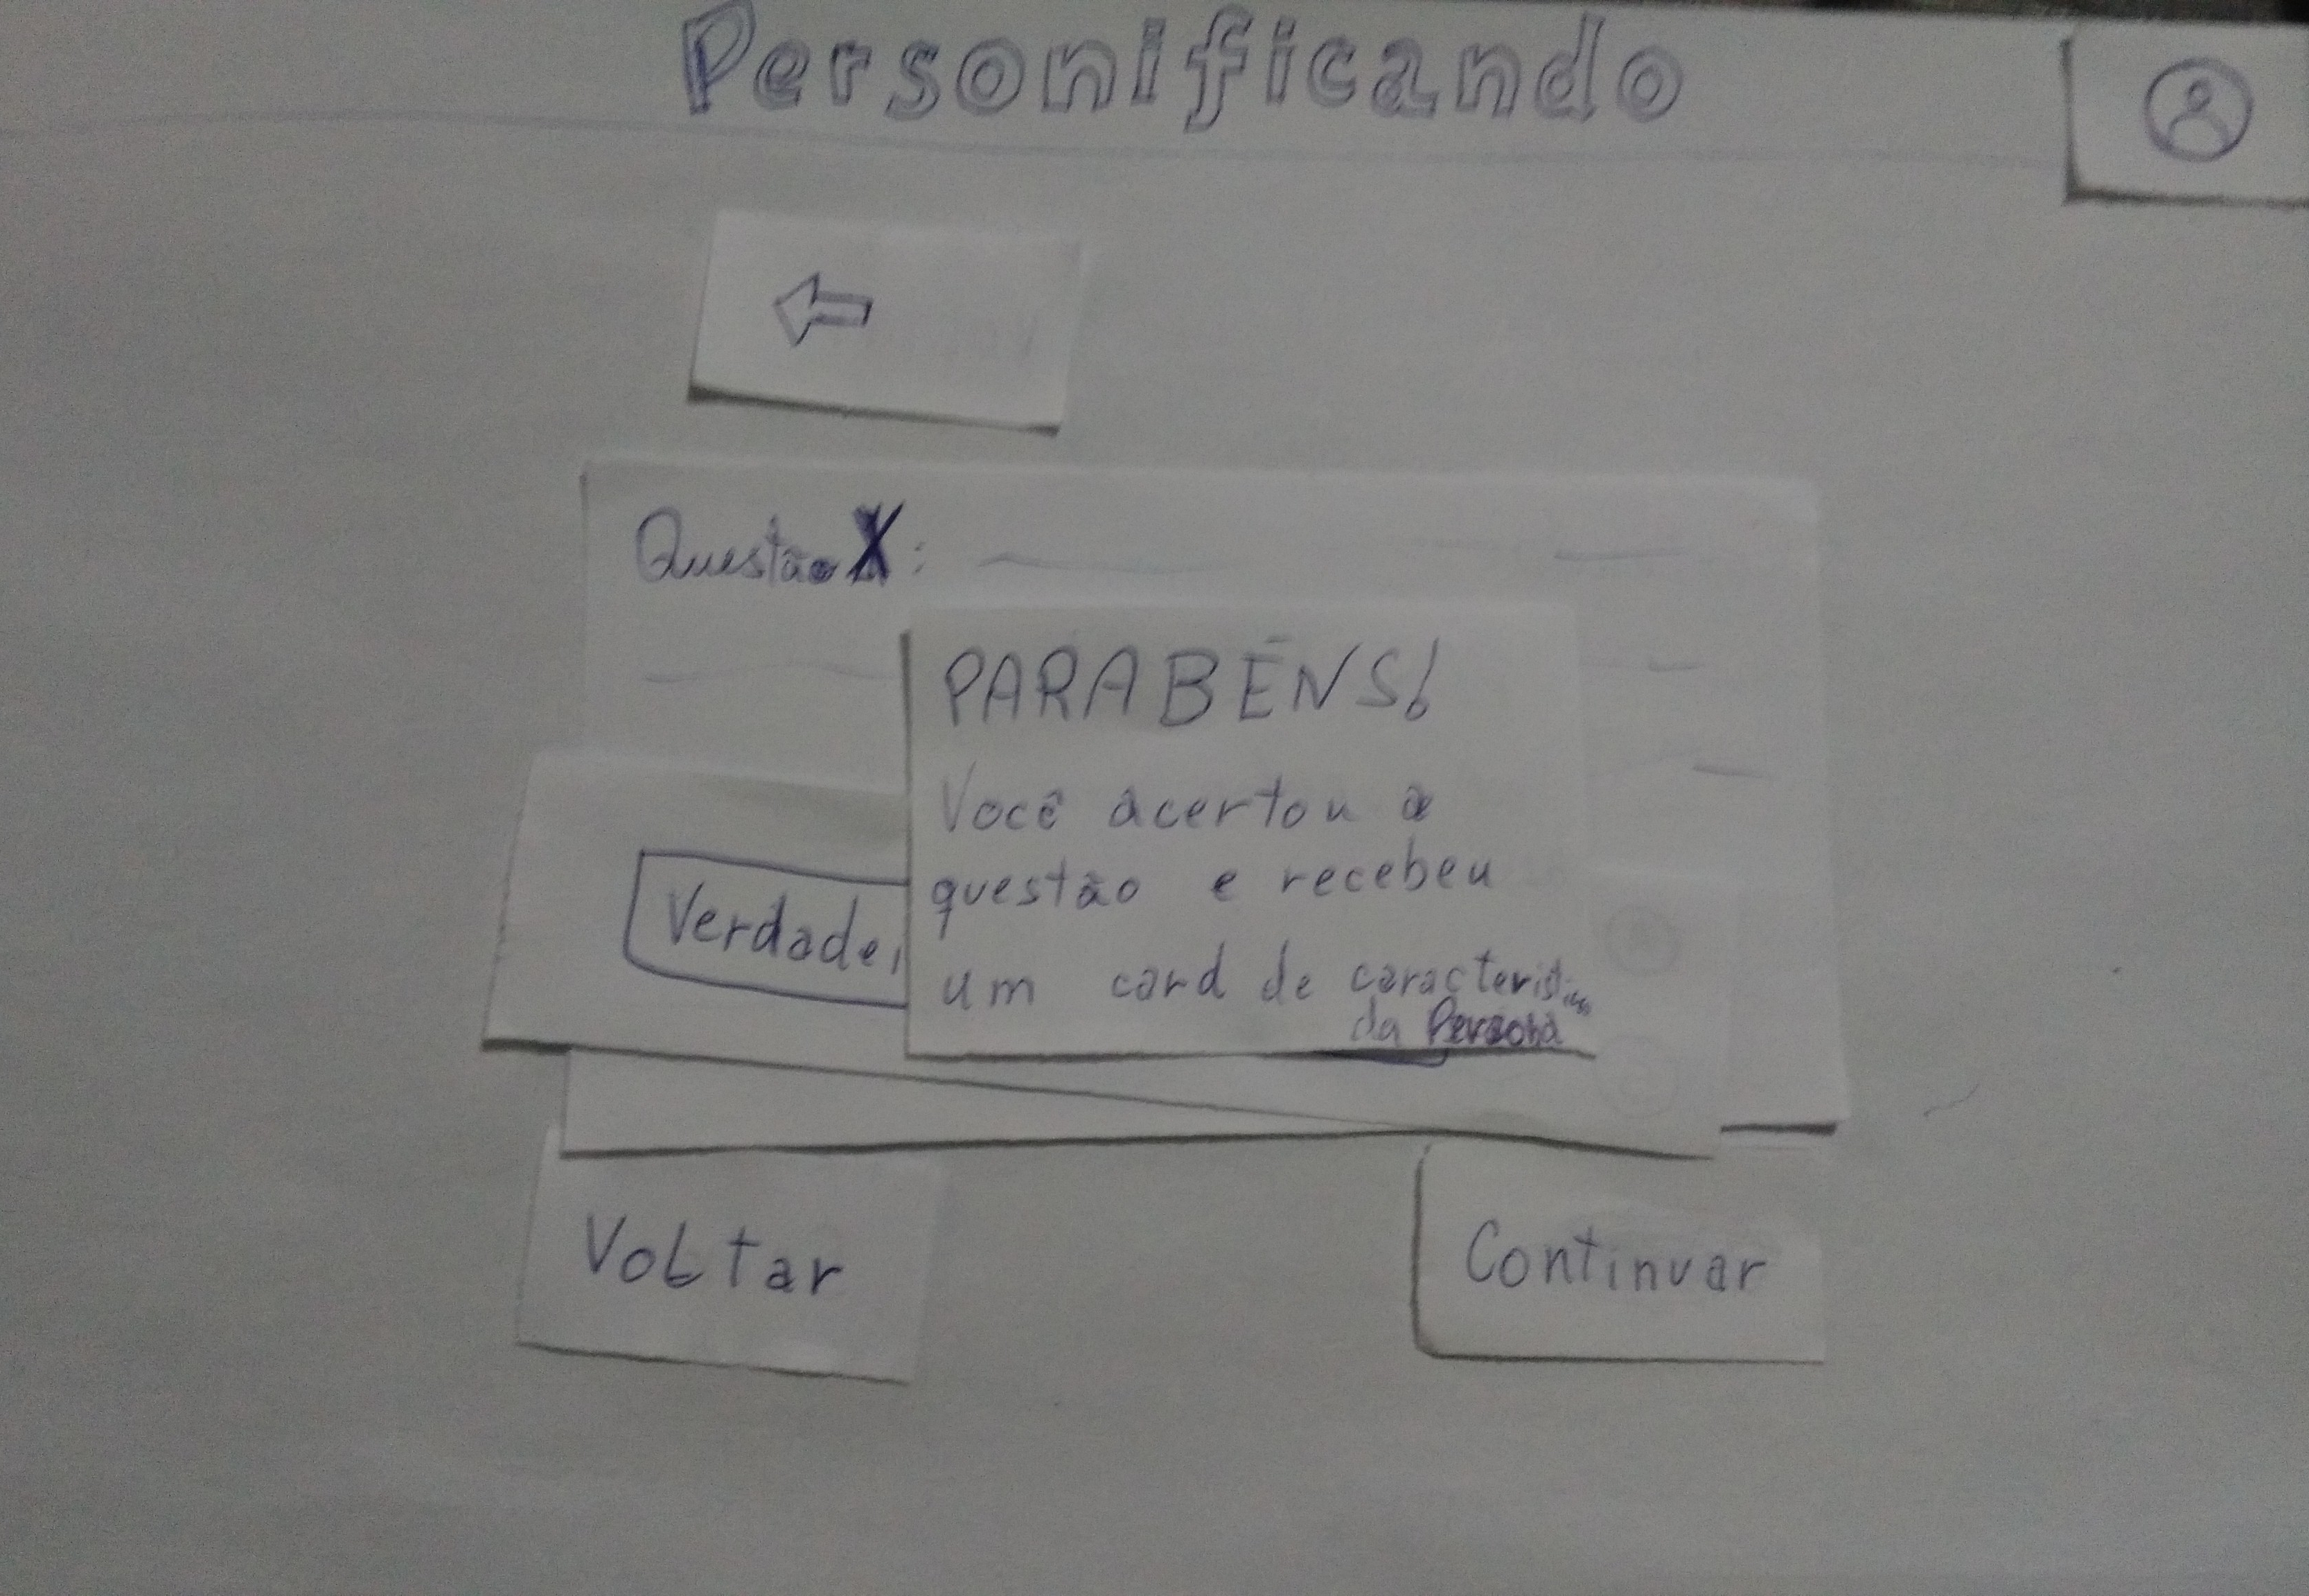
\includegraphics[keepaspectratio=true,scale=0.055]{figuras/prototype/proto13.jpg}
        \label{Fig:quest_recomp.png}
    }
    \quad
    \subfigure[Questão - Card de Persona]{
        \includegraphics[keepaspectratio=true,scale=0.055]{figuras/prototype/proto14.jpg}
        \label{Fig:quest_card.png}
    }
    \subfigure[Questão - Resposta Errada]{
        \includegraphics[keepaspectratio=true,scale=0.055]{figuras/prototype/proto15.jpg}
        \label{Fig:quest_erro.png}
    }
    \quad
    \subfigure[Questão - Correção da Resposta]{
        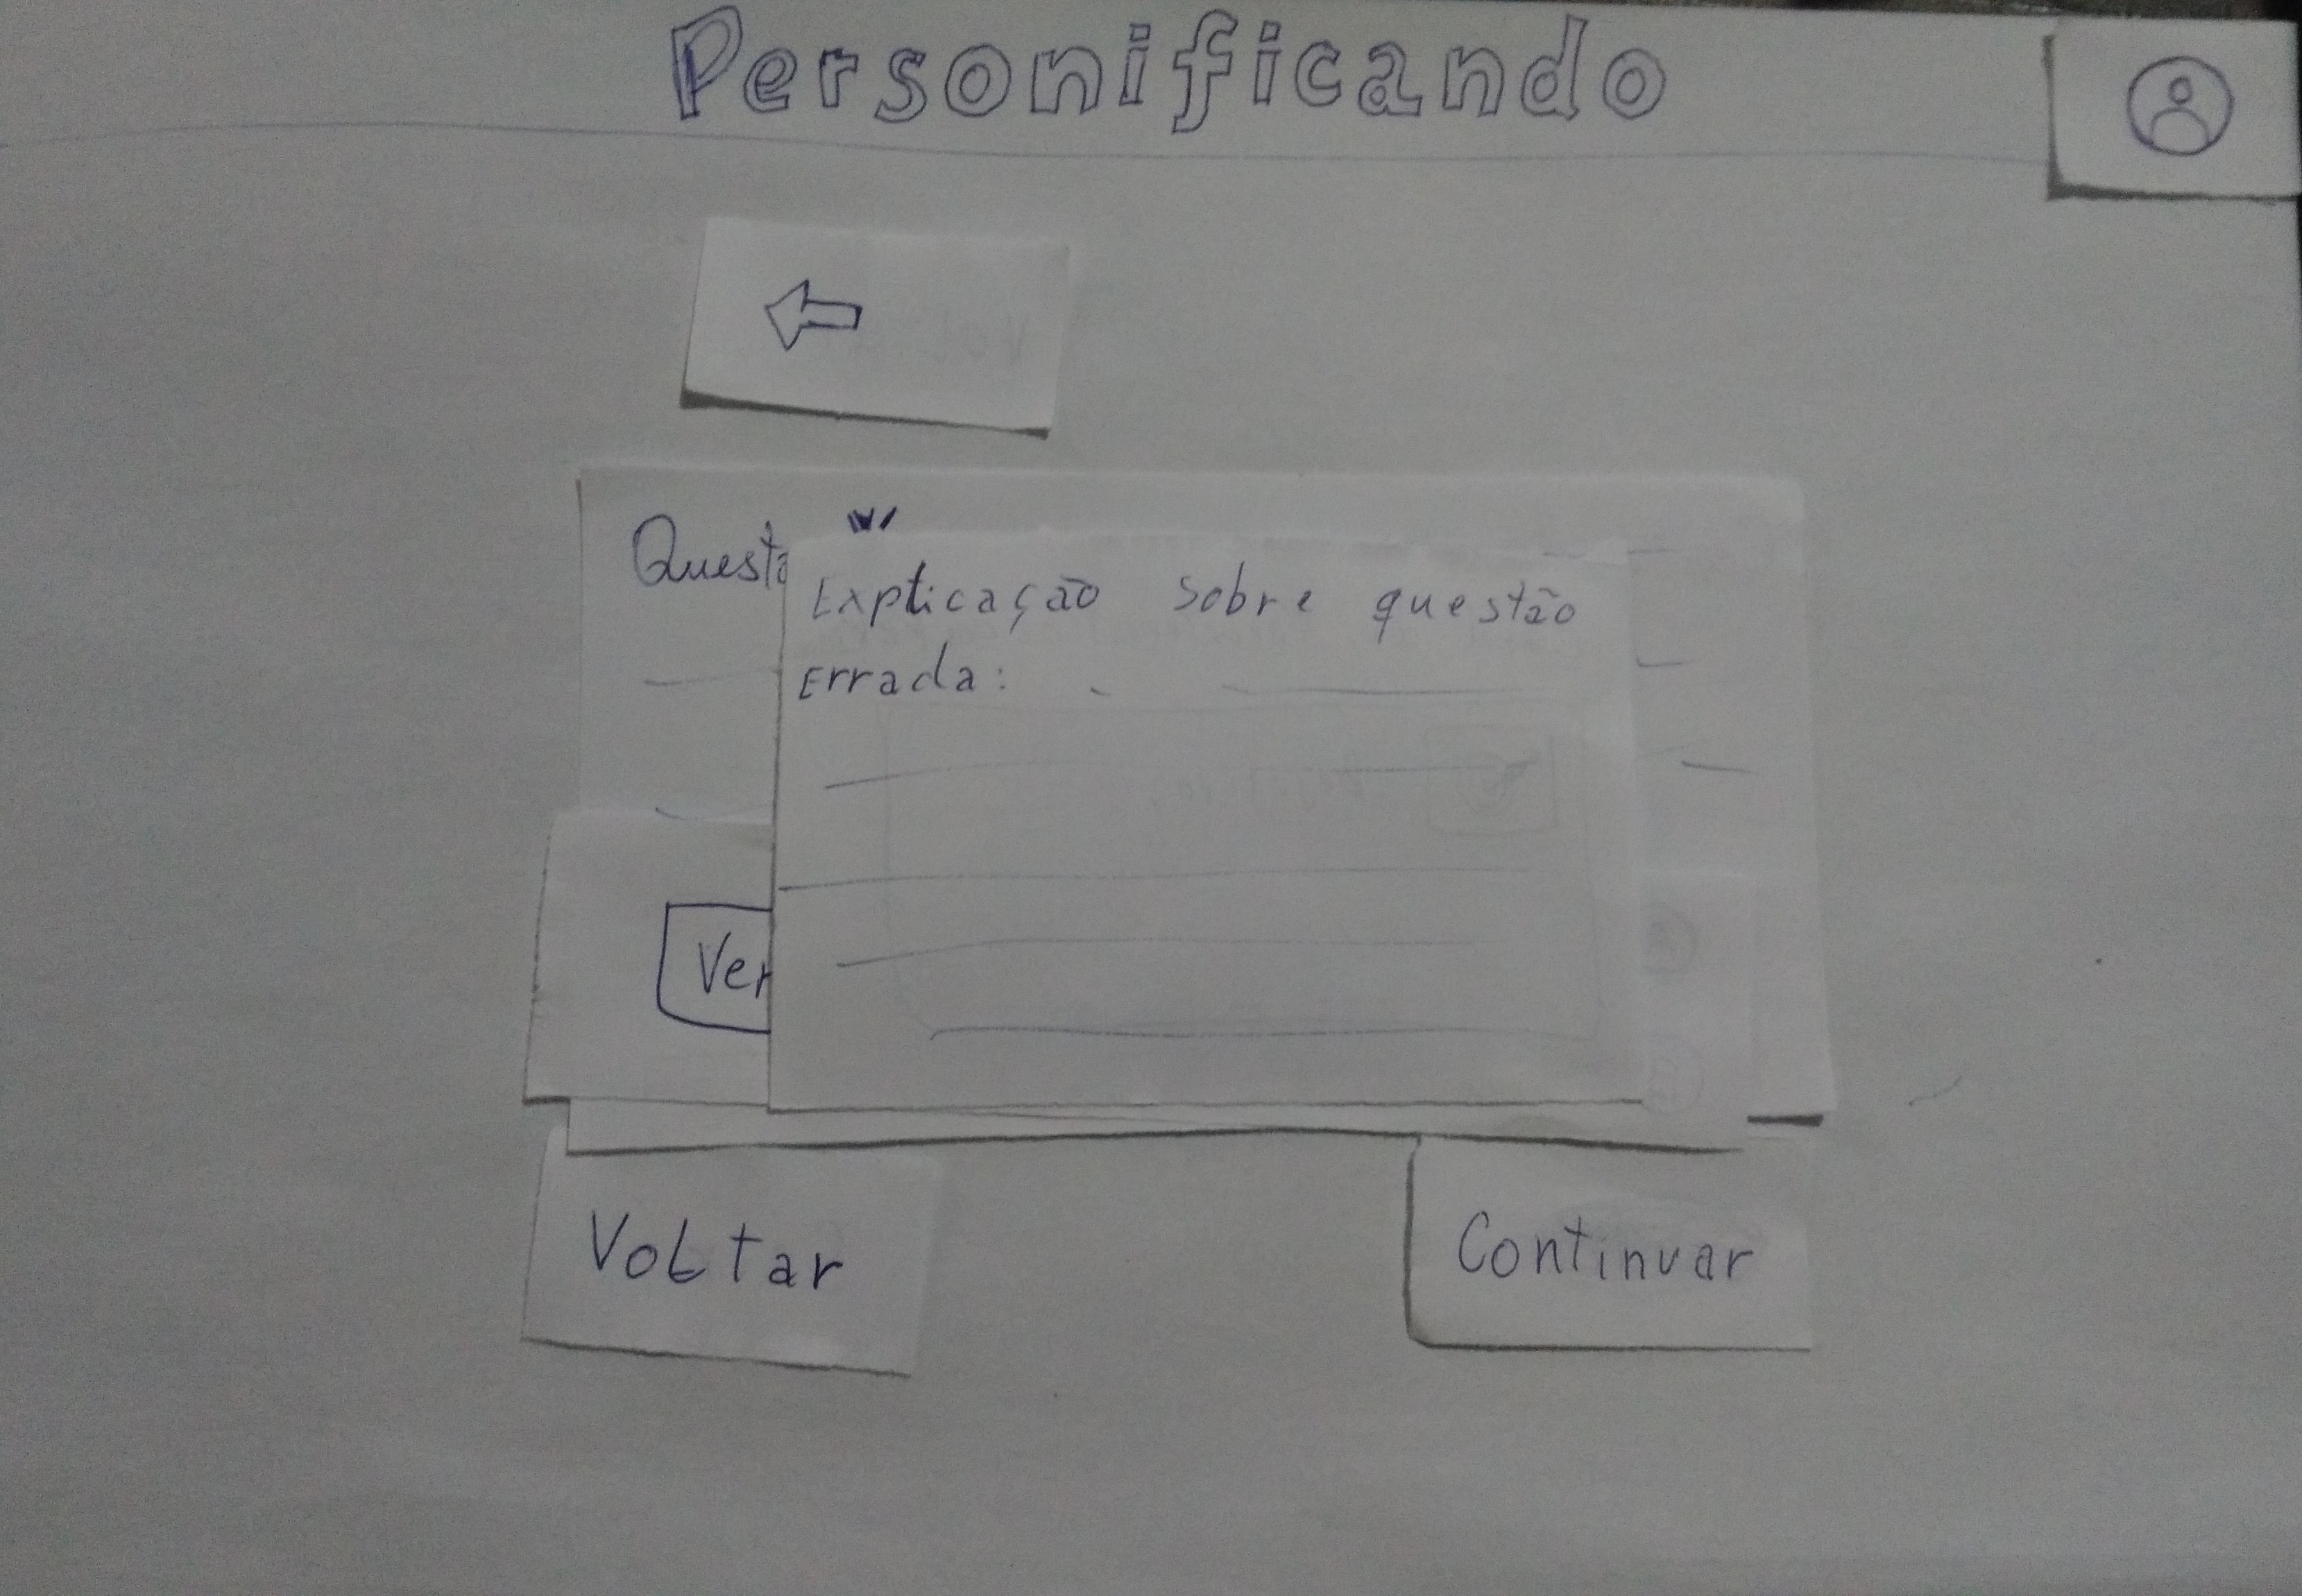
\includegraphics[keepaspectratio=true,scale=0.055]{figuras/prototype/proto16.jpg}
        \label{Fig:quest_correcao.png}
    }
    \quad
    \subfigure[Ambiente Personas]{
        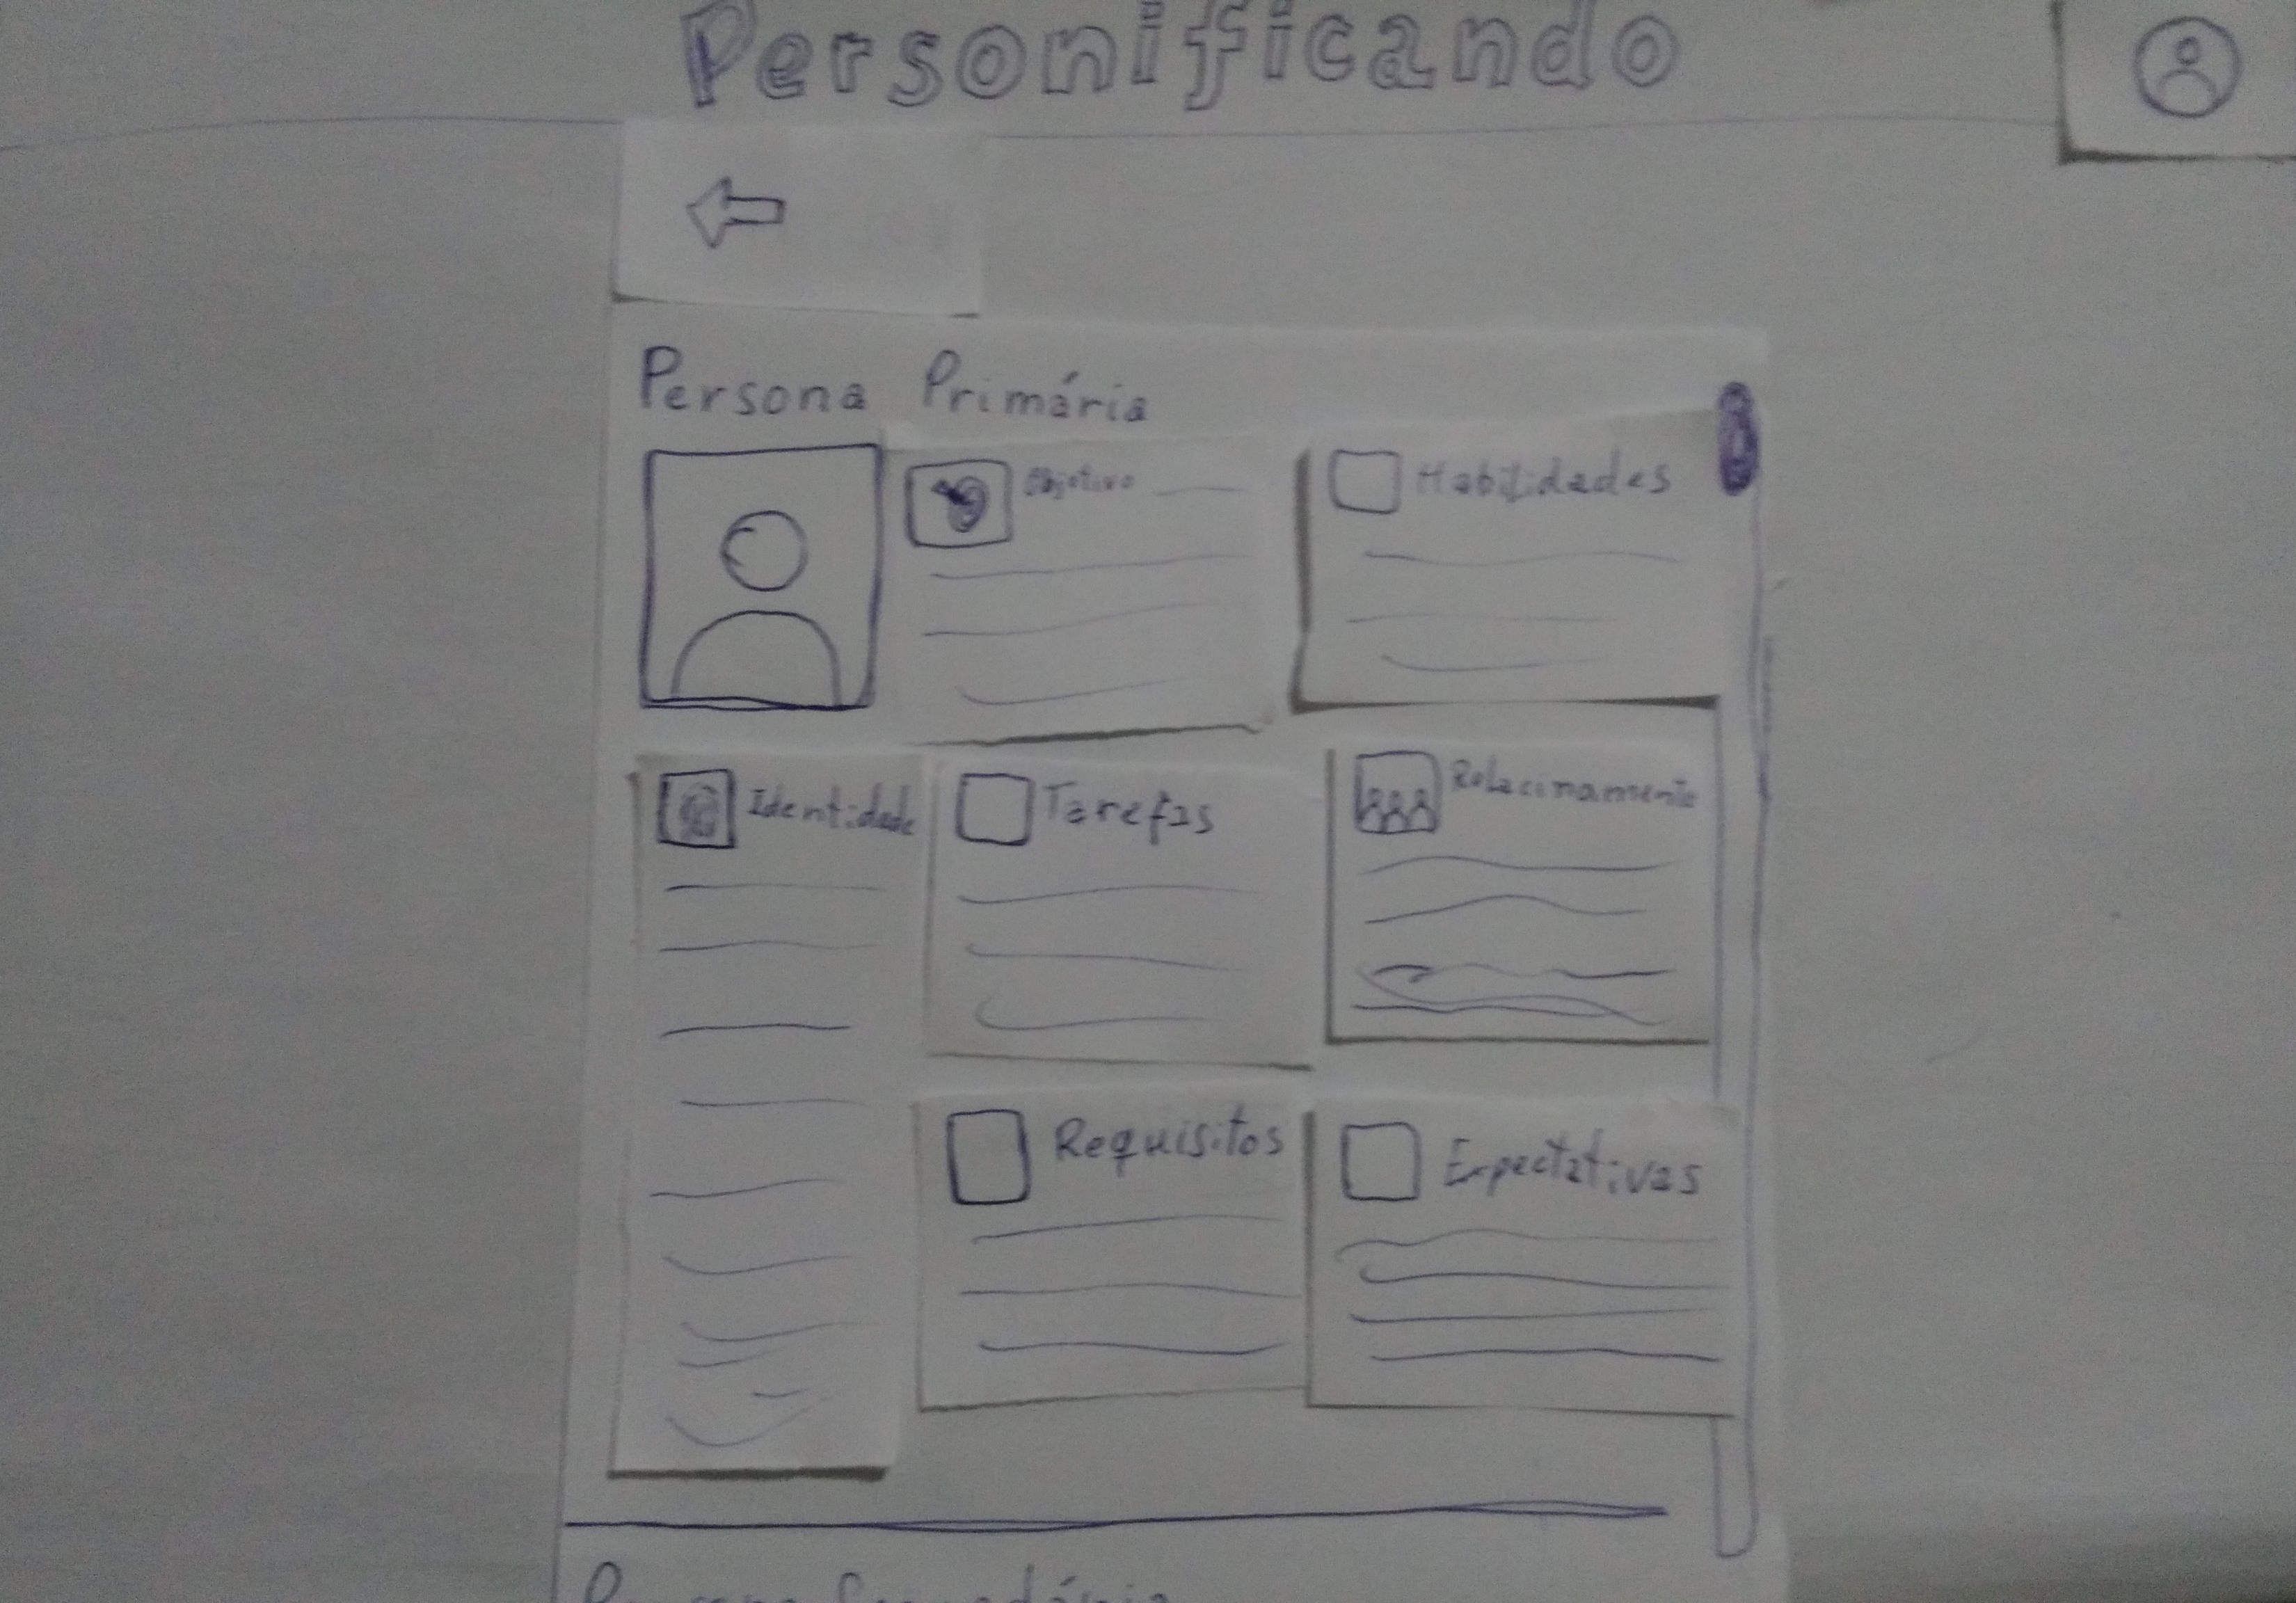
\includegraphics[keepaspectratio=true,scale=0.055]{figuras/prototype/proto17.jpg}
        \label{Fig:amb_pers.png}
    }
	\caption{Telas do Protótipo de Papel 3 - Próprio Autor}
	\label{Fig:proto3.png}
\end{figure}

\end{apendicesenv}